\documentclass[12pt,a4paper]{report}
\usepackage[utf8]{inputenc}
\usepackage{graphicx}
\graphicspath{ {C:/Users/kamila/Documents/Praca licencjacka/} }
\usepackage{amsmath}
\usepackage{tikz}
\usepackage{amsfonts}
\usepackage{latexsym}
\usepackage{amssymb}
\usepackage{amsthm}
\usepackage{paralist}
\usepackage{polski}
\usepackage{xcolor}
\usepackage{multicol}
\usepackage[hidelinks]{hyperref}
\usepackage{natbib} % potrzba do bibliografii
\usepackage[left=2cm,right=2cm,top=2cm,bottom=2cm]{geometry}
\usepackage{enumitem}
%\usepackage[acronym]{glossaries} COS NIE DZIALA WYWALA BLEDY

\usepackage{framed}
\usepackage{fancyvrb}


\author{Kamila Choja}
\title{Wybrane zastosowanie statystycznych metod porządkowania danych wielowymiarowych}


\newtheorem{theorem}{Twierdzenie}[section]
\newtheorem{definition}[theorem]{Definicja}
\newtheorem{uwaga}{Uwaga}
\newtheorem{example}{Przykład}
\newtheorem{stwierdzenie}{Stwierdzenie}
\newtheorem{wlasnosci}{Własności}

\newcommand{\setR}{\mathbb{R}}

\newcommand{\Lp}[2]{\operatorname{L}_{#1} \left( {#2} \right)}
\newcommand{\norm}[2][]{\left\| {#2} \right\|_{#1}}
\newcommand{\distance}[3][d]{\operatorname{#1}\left( {#2}; {#3}\right)}
\newcommand{\mediana}{\operatorname{med}}
\newcommand{\licznosc}[1]{\overline{\overline{#1}}}

\newcommand{\Ex}{\operatorname{E}}
\newcommand{\Variance}{\operatorname{Var}}


\newcommand{\closure}[1]{\overline{#1}}

\begin{document}
\begin{titlepage}
\begin{center}
        \vspace*{1cm}
        {\large POLITECHNIKA ŁÓDZKA}\\
       \vspace*{1cm}
        {\large WYDZIAŁ FIZYKI TECHNICZNEJ, INFORMATYKI I MATEMATYKI STOSOWANEJ}\\
        \vspace*{2cm}
    \end{center}        
        
\text{Kierunek: Matematyka}\\
\vspace*{0.3cm}
\hspace*{0.3cm}
\text{Specjalność: Matematyczne Metody Analizy Danych Biznesowych}
  
\begin{center}
\rule{\textwidth}{0.5pt}

\vspace*{0.5cm}
   
{\large WYBRANE ZASTOSOWANIE STATYSTYCZNYCH METOD\\ }
{\large PORZĄDKOWANIA DANYCH WIELOWYMIAROWYCH\\}
\vspace*{1cm}


\begin{flushright}
Kamila Choja\\
Nr albumu: 204052 
 \end{flushright}
\rule{\textwidth}{0.5pt}

Praca licencjacka\\
napisana w~Instytucie Matematyki Politechniki Łódzkiej\\

\vspace*{2cm}

Promotor: dr, mgr inż. Piotr Kowalski\\
\vfill
ŁÓDŹ, LIPIEC 2018


     \end{center}   
\end{titlepage}

\tableofcontents

\chapter{Wstęp}
Wielowymiarowa analiza danych jest istotnym pojęciem we współczesnej analizie. Pośród wielu zadań z~tej dziedziny, w~tej pracy chcemy skupić się na~zadaniu porządkowania danych, tj. wskazywaniu uporządkowania o~biektów, reprezentowanych przez wielowymiarowe dane. Przedstawione w~pracy rozwiązania mogą mieć zastosowanie do wielu problemów napotykanych w~codziennej pracy analityków. Do poprawnego zrozumienia zagadnienia statystycznego porządkowania danych należy jednak zgromadzić wiedzę i~teorię z~wielu o~bszarów matematyki i~statystyki o~raz zaprezentować ich zastosowanie w~praktycznych przykładach. Takie zgrupowanie wyżej wskazanych zagadnień jest głównym zadaniem niniejszej pracy. 

Praca została uporządkowana w~5 rozdziałach. Rozdział 1 stanowi bieżący wstęp. Z~kolei rozdział 2 zawiera potrzebne teorie różnych działów matematyki i~statystyki, które są wykorzystywane w~kolejnych częściach pracy. o~mówione są w~nim także zagadnienia dotyczące podstaw rachunku prawdopodobieństwa o~raz statystyki (sekcja \ref{rachunek prawdopodobienstwa}), niezbędne do rozumienia wielowymiarowych danych jako losowej próby prostej pewnej wielowymiarowej zmiennej losowej o~raz celem wprowadzenia jednolitych o~znaczeń. Znaczną część tego rozdziału poświęcamy matematycznej teorii porządków - tak liniowych jak i~częściowych, albowiem algorytmy prezentowane w~dalszych rozdziałach nawiązują do teorii porządków, definiowanej w~ramach współczesnej teorii mnogości. Z~uwagi na~fakt, iż nie wszystkie porządki wydobywane z~danych są porządkami liniowymi, o~mawiamy również podstawy o~raz wybrane elementy z~teorii grafów. Porządki częściowe mogą być bowiem prezentowane na~strukturach grafowych ze znakomitą korzyścią dla przejrzystości. o~prócz tego w~rozdziale 2 zawarliśmy też elementy teorii przestrzeni metrycznych, gdyż o~dległości pomiędzy wektorami danych są istotnym elementem w~prawie każdym z~omawianych algorytmów. Tutaj zawarte zostały również o~pisy podstawowych przekształceń na~zbiorach danych, wykorzystywanych na~etapie wstępnego ich przetwarzania.

Kluczowe teorie dotyczące samego porządkowania danych statystycznych zgromadzone są w~rozdziale 3. W~tej części pracy o~mawiane są również najistotniejsze sposoby wydobywania porządków z~danych statystycznych, prezentowana jest ich systematyka o~raz o~mawiane są właściwości o~raz o~dmiany. Podstawowy podział na: metody porządkowania liniowego - pozwalające o~kreślić ukryte porządki liniowe, o~raz metody nieliniowe - służące do wskazywania grafowych reprezentacji o~dkrytych porządków częściowych, rozdziela dwie główne sekcje tego rozdziału. Z~kolei w~rozdziale 4 przedstawiamy eksperymenty przeprowadzone celem lepszego zaprezentowania treści rozdziału 3. Dla potrzeb tej pracy został wytworzony zbiór wielowymiarowych danych - reprezentujący pewien podzbiór o~głoszeń znaczącego portalu z~ofertami sprzedaży pojazdów. Ponadto w~rozdziale tym o~pisujemy własne implementacje wybranych algorytmów z~rozdziału 3 o~pracowane w~języku R i~prezentujemy uzyskane porządki. W~rozdziale 5 zawarte jest treściwe podsumowanie, zarówno z~zakresu o~pisu statystycznych algorytmów porządkowania danych jak i~dla wyników przeprowadzonych eksperymentów.

%25.06
%W dalszej części pracy zostały o~pracowane podstawowe pojęcia teorii grafów \ref{grafy}, spowodowane to zostało interpretację graficzną częściowego uporządkowania zbioru, którego to metody statystyczne o~pracowane na~podstawie \citep{panek2013} zostały przedstawione o~bok metod porządkowania liniowego w~rozdziale \ref{metody porzadkowania}. Ze względu na~to również, że część praktyczna pracy, została w~większości o~parta na~podstawie  tej pozycji, użyłam przyjętych przez autora nazw statystycznych podziału relacji porządku, tj. metody porządkowania liniowego, natomiast metody będące o~dpowiednikiem relacji częściowego porządku zostały umieszczone pod nazwą metody porządkowania nieliniowego. Pozostając przy rozdziale \ref{metody porzadkowania} na~samym jego początku zostały o~mówione własności porządkowania liniowego, które to w~dalszej  kolejności zostały sformalizowane, a następnie udowodnione. 
%Ostatni rozdział pracy \ref{Zastosowanie} stanowi jej praktyczny aspekt. o~mówiłam w~nim stworzony przez siebie zbiór danych, na~którym to w~dalszej części pracy przetestowałam stworzone przez siebie implementacje wybranych metod porządkowania. Algorytmy zostały napisane w~programie R-Studio.  Na~koniec wyniki uporządkowań zostały porównane.
%25.06

%Przy metodach porządkowania warto wspomnieć o~ interpretacji geometrycznej uporządkowania. W~przypadku relacji częściowego porządku, interpretacją jest diagram Hassego, w~którym to dany o~biekt łączy jest z~drugim, gdy jeden jest poprzednikiem drugiego, a drugi jest następnikiem pierwszego. %%odwolanie do sekcji grafy slabe - pomyslec; moze niezbendym bylo o~pracowanie podstawowoych pojec z~teorii grafow, ze wzgledu na~to ze w~roddziale 3 - o~dwolanie, o~pracowanym na~podstawie ksiazki \cite{panek2013} zostały tam o~mówione statystyczne metody porządkowania - liniowe i~nieliniowe. Powracajac do ujecie matemtycznego, te drugie sa niczym innym jak interpretacja relacji czesciowego porzadku
%Jako że w~dalszej części pracy zostały przedstawione 
%%pomyslec o~dowloanie do grafu i~metod prozadkowania w~jendym
%Po wprowadzeniu powyższych pojęć, mogłam przejść do części praktycznej pracy tj. implementacji wybranych %zastosowań metod porządkowania. W~związku z~tym został stworzony rozdział 4 \ref{Zastosowanie}, w~którym to %omówiłam stworzony przez siebie zbiór o~biektów, a następnie zaprezentowałam własne algorytmy wybranych metod, które zostały o~pracowane z~wykorzystaniem R-Studio.




% W~ujęciu matematycznym porządkowanie jest niczym innym jak relacją porządku, który możemy podzielić na~porządek liniowy o~raz częściowy na~danym zbiorze. Ze względu na~to, w~sekcji \ref{teoria mnogosci} zostały o~pracowane wybrane pojęcia teorii mnogości, po to by w~dalszej części pracy móc przejść do  Niezbędnym również było wprowadzenie podstawowych pojęć rachunku prawdopodobieństwa, w~celu zrozumienia danych jako próby losowej, w~tym celu została stworzona sekcja \ref{rachunek prawdopodobienstwa}. Mając tak o~pracowane podstawy teoretyczne mogłam przejść do 

%W rozdziale 3 zostaną o~mówione implementacje porządku liniowego jak i~częściowego. Ze względu na~to, że część praktyczna pracy, została w~większości o~parta na~książce \cite{panek2013}, w~związku z~tym użyłam przyjętych przez autora nazw statystycznych podziału relacji porządku, tj. metody porządkowania liniowego, natomiast metody będące o~dpowiednikiem relacji częściowego porządku zostały umieszczone pod nazwą metody porządkowania nieliniowego. 

\chapter{Preliminaria}  

\section{Notacja} 

Poniżej znajduje się lista pojęć powszechnie używanych w~pracy wraz z~symbolami, które się im  przypisuje. 
  
\begin{itemize}
\item $\mathbb{R}$ - zbiór liczb rzeczywistych,
\item $\mathbb{N}$ - zbiór liczb naturalnych,
\item $K$ - o~znaczenie dowolnego ciała zbioru,
%\item $\licznosc{[1]}$ - liczność zbioru
%+-\item $\mathcal{E}^n$ - przestrzeń euklidesowa n-wymiarowa
\item $O = \{$O$_{1}$, o~$_{2}$, $\dots$, o~$_{n}\}$ - zbiór o~biektów przestrzennych, tj. o~pisywanych przez wiele atrybutów, $n \in \mathbb{N}$,
\item $X=[x_{ij}]$ - macierz surowych danych, gdzie $x_{ij}$-oznacza wartość $j$-tej zmiennej dla $i$-tego o~biektu, gdzie: $i=1,\ldots,n$, $j=1,\ldots, m,$, $n,m \in \mathbb{N}$. W~rozdziale drugim, przez $X$ najczęściej będziemy o~znaczać dowolny zbiór,
\item $N=[n_{ij}]$ - macierz znormalizowanych danych, gdzie $n_{ij}$ o~znacza wartość $j$-tej cechy $i$-tego o~biektu,
\item $x^{S}$ - o~znaczenie zmiennej mającej charakter stymulanty,
\item $x^{D}$ - o~znaczenie zmiennej mającej charakter destymulanty,
\item $x^{N}$ - o~znaczenie zmiennej mającej charakter nominanty,
\item $D=[d_{ik}]$ - o~znaczenie macierzy o~dległości, gdzie $d_{ik}$ o~znacza o~dległość między $i$-tym i~$k$-tym o~biektem, gdzie: $i, k=1,\ldots,n$, $n \in \mathbb{N}$,
\item $s_{i}$ - o~znaczenie zmiennej syntetycznej $i$-tego o~biektu,
\item $P_{0}=[n_{0j}]$ - o~znaczenie o~biektu wzorcowego, gdzie $n_{0j}$- znormalizowana $j$-ta współrzędna o~biektu wzorcowego,
\item $Y$ - w~rozdziale drugim używana jest najczęściej do o~znaczenie zmiennej losowej,
\item $\Omega$ - o~znaczenie dowolnej przestrzeni zdarzeń elementarnych $\omega$, z~rodziną podzbiorów $\mathcal{F}$,
%\item $\sigma$ -  sigma ciało zbiorów $\mathcal{F}$
\item $\mathcal{B}$ - rodzina zbiorów borelowskich,
\item $\mathfrak{B}$ - rodzina wszystkich zbiorów o~twartych, %https://www.sharelatex.com/learn/Mathematical_fonts
%\item $\mediana ( \cdot)$ - o~znaczać będzie mediany z~próby
\item $\leq$ - o~znaczenie relacji częściowego porządku, przy dołożeniu warunku spójności o~znaczać będzie relację liniowego porządku,
\item $\mediana{(\cdot)}$ - o~znaczenie mediany zbioru,
\item $\max{(\cdot)}$ - o~znaczenie maksymalnej wartości zbioru,
\item $\min{(\cdot)}$ - o~znaczenie minimalnej wartości zbioru,
\item $\licznosc{(\cdot)}$ - o~znaczenie mocy zbioru,
\item $G$ - o~znaczenie o~gólnego grafu prostego dla którego $V(G)$ jest zbiorem wierzchołków grafu, a $E(G)$ zbiorem jego krawędzi,


%\item $D$ - graf skierowany(digraf)
%\item $V(D)$ - zbiór wierzchołków digrafu $D$
%\item $A(D)$ - rodzina łuków digrafu $D$


\end{itemize}


\section{Słownik użytych pojęć}
W pracy zostały wykorzystane następujące pojęcia:
\begin{itemize}
%pojecia proby,statystyi, modelu - formalne mozna podac w~oparciu o~ wyklady Bartoszewicza i~pliku- "proba_mod staty_statytsyka folder: pliki pdf do pracy
\item Statystyka matematyczna \cite[w o~parciu o~ rozdział 1]{krysicki1999}\\
Statystyka matematyczna jest nauką zajmującą się o~pisywaniem i~analizą zjawisk przy użyciu metod rachunku prawdopodobieństwa. 


%\item Model statystyczny \cite[w o~parciu o~ rozdział 2]{bartoszewicz1996}
%Modelem statystycznym nazywamy przestrzeń próby doświadczenia tj. wartości zmiennych losowych o~ jednakowym rozkładzie, rodzinę podzbiorów zbioru zmiennych o~raz prawdopodobieństwo występowania danej zmiennej. Można tutaj wskazać analogię do rachunku prawdopodobieństwa, tj. uporządkowanej trójki $(\Omega,\mathcal{F},P)$.
 
 
\item Cecha statystyczna \cite[Rozdział 1]{krysicki1999}\\
Cecha statystyczna jest to właściwość wspólna dla danego zbioru o~bserwacji. Jej wartości pozwalają rozróżnić elementy zbioru między sobą. cechy statystyczne można podzielić na~te mierzalne, tj. ilościowe (np. długość, ciężar), o~raz niemierzalne tj. jakościowe (np. kolor, płeć, zawód, województwo).

\end{itemize}

W celu prezentacji dużych ilości danych, w~analizie danych korzysta się z~pojęcia macierzy. Poniżej zostanie przedstawiona formalna definicja macierzy o~raz definicja macierzy o~bserwacji, czyli zbiorze o~biektów o~pisywanych przez zmienne. %W rozdziale dotyczącym wybranych pojęć z~teorii mnogości, topologii o~raz algebry liniowej, zostanie podana jej algebraiczna definicja. 

\begin{definition}{Macierz \cite[Rozdział 1]{banaszak2002}}\\
Niech $K$ będzie ciałem i~$m, n \in \mathbb{N}$. Macierzą o~ $m$-wierszach, $n$-kolumnach i~o wyrazach z~$K$ nazywamy każdą funkcję postaci
$A: \{1,\ldots, m \} \times \{1, \ldots, n\} \rightarrow K$
\end{definition}

\begin{example}
Macierz $A$ o~ $m$-wierszach i~$n$-kolumnach najczęściej zapisuje się postaci $A=[a_{ij}]_{1\leq i~\leq m,  1\leq j\leq n}$, tj. 
$$
A= \begin{bmatrix}
a_{11} & a_{12} & \ldots & a_{1n} \\
a_{21} & a_{22} & \ldots & a_{2n}\\ 
\ldots & \ldots & \ldots & \ldots\\
a_{m1} & a_{m2} & \ldots & a_{mn} \\
\end{bmatrix}    
$$
\end{example}

\begin{uwaga}
W statystyce koncepcja matematyczna macierzy jest rozszerzana, gdyż niektóre kolumny mają wartości z~poza ciała zbioru liczb $\mathbb{R}$ (mogą być np. tekstem).
\end{uwaga}

\begin{definition}{Macierz o~bserwacji \cite[Rozdział 2]{mlodak2006}}\\
Niech $m>1$ o~raz $n>1$ będą liczbami naturalnymi.  Macierzą o~bserwacji nazywamy macierz rozmiaru  $n \times m$  postaci
$$
X= \begin{bmatrix}
x_{11} & x_{12} & \ldots & x_{1m} \\
x_{21} & x_{22} & \ldots & x_{2m}\\
\ldots & \ldots & \ldots & \ldots \\
x_{n1} & x_{n2} & \ldots & x_{nm}\\
\end{bmatrix}
$$
gdzie:
$x_{ij}$ - zaobserwowana wartość $j$-tej cechy dla $i$-tego o~biektu.
\end{definition}


\begin{definition}{Macierz o~dległości zmiennych \cite[Rozdział 1.6]{panek2013}}\\
Macierzą o~dległości cech zmiennych nazywamy macierz, której elementami są o~dległości między parami badanych o~biektów: 
\begin{center}
$D = [d_{ik}].$
\end{center}
gdzie:\\
$d_{ik}$-odległość między $i$-tym a $k$-tym o~biektem, dla $i,k=1,2,\ldots,n$
\end{definition}

\begin{uwaga}
Zauważmy, że macierz o~bserwacji nie musi być symetryczna, z~kolei w~przypadku macierzy o~dległości jest to wymagane.
\end{uwaga}

W statystyce posługujemy się pojęciami skal do o~pisu różnych typów danych, które przyjmowane przez nas mogą podlegać analizie. W~związku z~powyższym zdefiniujmy następujące rodzaje skal:

\begin{itemize}


\item Skala porządkowa \cite[Rozdział 1.2]{panek2013}\\
Zmienna o~pisana jest na~skali porządkowej jeśli jej zbiór wartości jest zbiorem, w~którym wprowadzony jest porządek np. porządek liczb. Nie zawsze porządek ten jest ustalony w~sposób matematyczny. W~przypadku rozpatrywania zmiennych jakościowych, porządek ustalamy na~podstawie o~pinii ekspertów lub o~gólnie przyjętych poglądów np. poziom wykształcenia, o~ceny w~systemie szkolnym. 


\item Skala przedziałowa \cite[Rozdział 1.2]{panek2013}\\
Zmienna jest o~pisana na~skali przedziałowej gdy podobnie jak na~skali porządkowej jej zbiór wartości jest zbiorem uporządkowanym z~wprowadzoną funkcją o~dległości. Dodatkowo na~skali tej możliwe jest wyznaczenie umownego punktu - zera. Przykład zmiennych przedstawianych na~skali przedziałowej to: temperatura, czas.

%27.06
%Jest to skala, która w~odróżnieniu do skali porządkowej, pozwala o~bliczyć o~dległość między o~biektami, przy pomocy pomiaru cech, o~pisujących o~biekt. Skala ta może korzystać z~operacji dodawania o~raz o~dejmowania. Dla skali tej istnieje charakterystyczna wartość - punkt zerowy. Jest o~n wyznaczany w~sposób umowny, punkt ten pozwala zachować różnice między wartościami cechy, w~momencie zamiany jednostek miary. Przykład zmiennych przedstawianych na~skali przedziałowej: temperatura, rok urodzenia.
%27.06
 %Wartość zerowa na~tej skali ma charakter umowny, co prowadzi do zachowania różnic między wartościami cechy, przy zmianie jednostek miary. 

\item Skala ilorazowa \cite[Rozdział 1.2]{panek2013}\\
Zmienna jest o~pisana na~skali ilorazowej, jeśli jej zbiór wartości jest zbiorem postaci $[0, \infty)$ będący podzbiorem zbioru liczb $\mathbb{R}$, lub też taki zbiór wartości który można utożsamić z~podzbiorem liczb $\mathbb{R}$. Przykłady zmiennych o~pisywanych na~skali ilorazowej: napięcie elektryczne, bezrobocie. 

%26.05
%Skala ta, podobna jest do skali przedziałowej, z~tym że występuje w~niej zero bezwględne - punkt, który mówi o~ tym, że dana zmienna nie występuje, o~raz o~granicza lewostronnie zakres skali ilorazowej. Dzięki temu punktowi o~prócz działań dodawania i~odejmowania, można korzystać z~dzielenia o~raz mnożenia, co pozwala na~przedstawieniu dowolnej wartości cechy danego o~biektu, jako wielokrotna wartość cechy innego o~biektu. Przykład zmiennych przedstawianych na~skali ilorazowej: napięcie elektryczne, bezrobocie, inflacja.
%26.05

\end{itemize}

\begin{uwaga}
Jeżeli zmiennej o~pisującej dany o~biekt nie da się o~dnieść do żadnej z~powyższych skal, to zmienna ta nazywana jest nominalną.
\end{uwaga}

Ze względu na~to, że zmienne o~pisujące o~biekty mogą mieć różny charakter, poniżej zostały wprowadzone definicje trzech różnych typów zmiennych, którymi posługujemy się w~statystyce. 

\begin{definition}{Stymulanta \cite[Rozdział 1.5]{panek2013}}\\
Stymulantami nazywane są te zmienne (cechy), dla których pożądane są wysokie wysokie wartości w~badanych o~biektach, ze względu na~rozpatrywane zjawisko. 
\end{definition}

\begin{definition}{Destymulanta \cite[Rozdział 1.5]{panek2013}}\\
Destymulantami nazywane są te  zmienne, dla których niepożądane są wysokie wysokie wartości w~badanych o~biektach, ze względu na~rozpatrywane zjawisko. 
\end{definition}

\begin{definition}{Nominanta \cite[Rozdział 1.5]{panek2013}}\\
Nominantami nazywane są te zmienne, które mają o~kreśloną najkorzystniejszą wartość. o~dchylenia o~d tej wartości są niepożądane, ze względu na~rozpatrywane zjawisko. 
\end{definition}



\section{Podstawowe pojęcia rachunku prawdopodobieństwa o~raz statystyki} \label{rachunek prawdopodobienstwa}


Na potrzeby pracy, zostały wykorzystane pojęcia rachunku prawdopodobieństwa o~raz statystyki, konieczne do zrozumienia danych jako próby losowej. W~tym celu niezbędne było wprowadzenie definicji prawdopodobieństwa, zmiennej losowej, a także pojęć powiązanych z~tymi definicjami tj. ciała zbiorów, $\sigma$-ciała zbiorów, przestrzeni zdarzeń elementarnych, zdarzenia losowego.


\begin{definition}{Ciało zbiorów \cite[Rozdział 8.1]{rudnicki2006}}\\
Rodzinę $\mathcal{F}$ podzbiorów, niepustego zbioru $X$ nazywamy ciałem zbiorów, jeżeli spełnia o~na następujące warunku: 
\begin{enumerate}
\item $\emptyset \in \mathcal{F}$,
\item jeżeli $A \in \mathcal{F}$, to $X \setminus A \in \mathcal{F}$,
\item jeżeli $A \in \mathcal{F}$, to $A \cup B \in \mathcal{F}$.
\end{enumerate}
\end{definition}


\begin{definition}{$\sigma$-algebra/ciało zbiorów\cite[Rozdział 8.1]{rudnicki2006}}\\
Ciało zbiorów $\mathcal{F}$ nazywamy $\sigma$-ciałem zbiorów, jeżeli spełnia o~na warunek
dla dowolnych zbiorów $A_{n} \in \mathcal{F}, n \in \mathbb{N}$, mamy
$\bigcup\limits_{i=1}^{\infty} A_n \in \mathcal{F}$.
%Elementy $\sigma$-ciała $\mathcal{F}$ nazywamy zbiorami mierzalnymi.
\end{definition}
Najważniejszym $\sigma$-ciałem zbiorów w~matematyce są $\sigma$-ciała zbiorów Borelowskich, dlatego też wprowadzimy definicję zbiorów borelowskich. 



\begin{definition}{Zbiory borelowskie \cite[w o~praciu o~ rozdział 2]{billingsley1987}}\\
Zbiorami borelowskimi względem danej przestrzeni $X$, nazywamy zbiory należące do $\sigma$-ciała $X$ generowanego przez rodzinę $\mathfrak{B}(X)$ - wszystkich zbiorów o~twartych w~$X$. Rodzinę wszystkich zbiorów borelowskich względem $X$, o~znaczamy $\mathcal{B}(X)$.
\end{definition}

$\sigma$-ciała zbiorów często mogą być po prostu utożsamiane ze zbiorami, które można zmierzyć, w~związku z~tym wprowadzimy definicję miary zbioru.

\begin{definition}{Miara zbioru \cite[Rozdział 2.10] {billingsley1987}}\\
Funkcję $\mu$ o~kreśloną na~ciele $\mathcal{F}$ podzbiorów zbioru $\Omega$ nazywamy miarą, jeśli spełnia następujące warunki: 
\begin{enumerate}
\item $\forall{\textit{A} \in \mathcal{F}} \quad \mu(A) \in [0, \infty]$ ,
\item $\mu(\emptyset)=0$,
\item jeśli $A_1, A_2,...$ jest ciągiem rozłącznych zbiorów $\mathcal{F}$-mierzalnych takich, że $\bigcup\limits_{k=1}^{\infty} A_k \in \mathcal{F}$, to 

$$\mu\big(\bigcup\limits_{k=1}^{\infty} A_k\big)=\sum_{k=1}^{\infty} \mu(A_k).$$

\end{enumerate}
\end{definition}


\begin{definition}{Przestrzeń mierzalna \cite[Rozdział 2.10]{billingsley1987}}\\
Przestrzenią mierzalną nazywamy parę $(X, \mathcal{F})$, gdzie $\mathcal{F}$ jest $\sigma$-ciałem podzbiorów zbioru $X$
\end{definition}


\begin{definition}{Funkcja mierzalna \cite[w o~parciu o~ rozdział 8.2]{rudnicki2006}}\\
Niech $X$ będzie niepustym zbiorem, $\mathcal{F}$  $\sigma$-ciałem na~$X$ i~$\overline{\mathbb{R}} = \mathbb{R} \cup \{-\infty, \infty \}$. Funkcję $f: X \rightarrow \overline{\mathbb{R}}$ nazywamy mierzalną, jeżeli zbiór $\{ x \in X: f(x) > a \}$ jest mierzalny przy dowolnym $a \in \mathbb{R}$.
\end{definition}

Mając powyższe definicje, wprowadźmy możemy wprowadzić poszukiwane definicje rachunku prawdopodobieństwa. 

\begin{definition}{Przestrzeń zdarzeń elementarnych \cite[w o~parciu o~ rozdział 1.1]{krysicki1999}}\\
Zbiór wszyskich możliwych wyników doświadczenia losowego nazywamy przestrzenią zdarzeń elementarnych i~oznaczamy przez $\Omega$. Elementy zbioru $\Omega$ nazywamy zdarzeniami elementarnymi i~oznaczamy $\omega$.
\end{definition}

\begin{definition}{Zdarzenie losowe \cite[w o~parciu o~ rozdział 1.1]{krysicki1999}}\\
Zdarzeniem losowym (zdarzeniem) nazywamy każdy podzbiór $\textit{A}$ zbioru $\Omega$, taki że  $A \in \mathcal{F}$, gdzie $\mathcal{F}$ jest rodziną podzbiorów $\Omega$ spełniającą następujące warunki:
\begin{enumerate}
\item $\Omega \in \mathcal{F}$,
\item Jeśli $A \in \mathcal{F}$, to $\textit{A$'$} \in \mathcal{F}$, gdzie $\textit{A$'$} = \Omega \setminus A $ jest zdarzeniem przeciwnym do zdarzenia $\textit{A}$,
\item Jeśli $\textit{A}_{i} \in \mathcal{F}$, $i= 1, 2, ...$,to $\bigcup\limits_{i=1}^{\infty} A_{i} \in \mathcal{F}. $
\end{enumerate}
Rodzinę $\mathcal{F}$ spełniającą warunki 1 - 3 nazywamy $\sigma$-ciałem podzbiorów zbioru $\Omega$
\end{definition}


\begin{definition}{Prawdopodobieństwo \cite[w o~parciu o~ rozdział 1.1]{krysicki1999}}\\
Prawdopodobieństwem nazywamy dowolną funkcję $P$ o~ wartościach rzeczywistych, o~kreśloną na~$\sigma$-ciele zdarzeń $\mathcal{F} \subset 2^\Omega$, spełniającą warunki: 
\begin{enumerate}
\item $\forall{\textit{A} \in \mathcal{F}} \quad \textit{P(A)} \geq 0,$
\item $\textit{P}(\Omega) = 1,$
\item Jeśli $\textit{A}_{i} \in \mathcal{F}$, $i= 1, 2, ...$ o~raz $A_{i} \cap A_{j} = \emptyset $ dla $i \neq j$, to 
\end{enumerate}

$$P \Big(\bigcup\limits_{i=1}^{\infty} A_{i} \Big)=\sum_{i=1}^{\infty} P(A_{i}). $$

\end{definition}


\begin{definition}{Przestrzeń probabilistyczna \cite[w o~parciu o~ rozdział 1.2]{krysicki1999}}\\
Przestrzenią probabilistyczną nazywamy uporządkowaną trójkę $(\Omega, \mathcal{F}, P)$, gdzie $\Omega$ jest zbiorem zdarzeń elementarnych, $\mathcal{F}$ jest $\sigma$-ciałem podzbiorów $\Omega$, zaś $P$ jest prawdopodobieństwem o~kreślonym na~$\mathcal{F}$.
\end{definition}

Dla tak podanej definicji prawdopodobieństwa, definiujemy:

\begin{definition}{Zmienna losowa \cite[Rozdział 2.1]{krysicki1999}}\\
Niech $(\Omega, \mathcal{F}, P)$ będzie dowolną przestrzenią probabilistyczną. Dowolną funkcję $\textit{Y} : \Omega \rightarrow \mathbb{R}$ nazywamy zmienną losową jednowymiarową, jeśli dla dowolnej liczby rzeczywistej $y$ zbiór zdarzeń elementarnych $\omega$, dla których spełniona jest nierówność $Y(\omega)< y$ jest zdarzeniem, czyli 
$$\{\omega: Y(\omega) < y \} \in \mathcal{F}\quad \forall y \in \mathbb{R}.$$

\end{definition}


\begin{definition}{Wektor losowy \cite[Rozdział 5.1]{jakubowski2004}}\\
Wektorem losowym nazywamy o~dwzorowanie $Y:\Omega \rightarrow \mathbb{R}^n$, spełniające następujący warunek: dla każdego układu liczb $t_1,t_2,\ldots,t_n \in \mathbb{R}^n$ zbiór $Y^{-1}((-\infty,t_1]\times \ldots \times(-\infty,t_n])$ należy do $\mathcal{F}$.
\end{definition}


\begin{definition}{Rozkład prawdopodobieństwa zmiennej losowej \cite[Rozdział 5.1]{jakubowski2004}}\\
Rozkładem prawdopodobieństwa zmiennej losowej $Y$ o~ wartościach w~$\mathbb{R}$ nazywamy funkcję $\mu_Y$ o~kreśloną na~$\mathcal{B}(\mathbb{R})$ zależnością:
$$\mu_Y(B)=P_Y(B)=P(Y^{-1}(B)), \quad B \in \mathcal{B}(\mathbb{R}).$$
 
\end{definition}


\begin{definition}{Rozkład dyskretny \cite[Rozdział 5.1]{jakubowski2004}}\\
Mówimy, że zmienna losowa jednowymiarowa $Y$ ma rozkład dyskretny, jeśli istnieje przeliczany zbiór $S \subset \mathbb{R}$, taki że $\mu_Y(S)=1$.
\end{definition}


\begin{definition}{Gęstość i~rozkład ciągły \cite[Rozdział 5.1]{jakubowski2004}}\\
Jeśli $\mu$ jest rozkładem prawdopodobieństwa na~$\mathbb{R}$ i~istnieje całkowalna funkcja $f: \mathbb{R} \rightarrow \mathbb{R}$ taka, że:
$$\mu(A)=\int_A f(y)dy,   A\in \mathcal{B}(\mathbb{R})  $$  %\quad dla \quad wszystkich
to funkcję $f$ nazywamy gęstością rozkładu $\mu$. Rozkład, który ma gęstość, nazywamy rozkładem ciągłym. 
\end{definition}


%\begin{definition}{Wektor losowy n-wymiarowy \cite[Rozdział 1]{bartoszewicz1996}\\}
%Wektorem losowym n-wymiarowym nazywamy funkcję $X: \Omega \rightarrow \mathbb{R}^n$ mierzalną względem $\sigma$-ciała $\mathcal{F}$ ($\mathcal{F}$-mierzalną), tzn. taką, że $X^{-1}(B) \in \mathcal{F}$ dla każdego $B \in \mathfrak{B}^n$.
%\end{definition}

\begin{definition}{Wartość o~czekiwana \cite[Rozdział 2.6]{krysicki1999}}\\
Niech $X$ będzie zmienną losową typu dyskretnego lub ciągłego. Wartością o~czekiwaną zmiennej losowej $Y$ nazywamy:

$$
\Ex (Y)=\left\{ \begin{array}{ll}
\sum\limits_{i=1}^{n} {y_ip_i}, & \textrm{jeśli zmienna ma rozkład dyskretny i~przyjmuje dokładnie $n$ wartości, }\\ 
\sum\limits_{i=1}^{\infty} {y_ip_i}, & \textrm{jeśli zmienna przyjmuje nieskończenie, ale przeliczalnie wiele wartości,}\\
\int\limits_{-\infty}^{\infty} {yf(y)dy}, & \textrm{jeśli zmienna ma rozkład ciągły.}
\end{array} \right.
$$

\end{definition}


\begin{definition}{Wariancja \cite[Rozdział 5.6]{jakubowski2004}}\\
Niech $Y$ będzie zmienną losową. Jeśli $\mathrm{E}(Y-\mathrm{E}Y)^2 < \infty$, to liczbę tę nazywamy wariancją zmiennej losowej Y o~ wartościach rzeczywistych i~oznaczamy: 
$$\Variance Y= \mathrm{E}(Y-\mathrm{E}Y)^2.$$
\end{definition}


\begin{definition}{Odchylenie standardowe \cite[Rozdział 5.6]{jakubowski2004}}\\
Niech $Y$ będzie zmienną losową. o~dchyleniem standardowym zmiennej losowej $Y$ nazywamy pierwiastek z~wariancji:
$$\sigma_Y=\sqrt{\Variance Y}.$$

\end{definition}

\begin{definition}{Próba losowa n-elementowa \cite[Rozdział 2]{bartoszewicz1996}}\\
Niech $(\Omega, \mathcal{F}, P)$ będzie przestrzenią probabilistyczną, zaś $Y_{i}:\Omega^{n}  \rightarrow \mathbb{R}$ będzie zmienną losową.  
Próbą losowa $n$-elementową nazywamy $n$-elementowy ciąg niezależnych zmiennych losowych o~ jednakowym prawdopodobieństwie, tzn. ciąg postaci $(\omega_{1}, \omega_{2}, \ldots, \omega_{n}) \in \Omega^{n}$, taki że $Y_{i}(\omega_{1}, \omega_{2}, \ldots, \omega_{n})=Y(\omega_{i})$.
\end{definition}


\begin{uwaga}
Powyższa definicja próby losowej jest wyrażona w~języku rachunku prawdopodobieństwa. W~języku statystyki próbę losową rozumiemy jako wartość pochodząca z~realizacji takiego doświadczenia.
\end{uwaga}



\begin{definition}{Rozkład normalny (Gaussa) \cite[Rozdział 5.10]{jakubowski2004}}\\
Jeśli zmienna losowa $Y$ ma gęstość postaci
$$
f(y)=\frac{1}{\sqrt{2\pi}\sigma}e^\frac{-(y-\mu_Y)^2}{2\sigma^2}
$$ 
dla $y \in \mathbb{R}$ i~pewnych $\mu_Y \in \mathbb{R}$ i~$\sigma^2 >0$. To mówimy, że zmienna losowa ma rozkład normalny z~parametrami $\mu$ i~$\sigma^2$, co zapisujemy $\mathcal{N}(\mu, \sigma^2)$.\\
W przypadku, gdy $\mu=0$ i~$\sigma^2=1$, to rozkład ten nazywamy standardowym rozkładem normalnym i~oznaczamy $\mathcal{N}(0,1)$, a gęstość jest postaci
$$f(y)=\frac{1}{\sqrt{2\pi}}e^\frac{-(y)^2}{2}.$$ 
\end{definition}


%\begin{definition}{Wartość o~czekiwana macierzy losowej $X$ \cite[Rozdział 1.3]{bartoszewicz1996}\\}
%Wartością o~czekiwaną macierzy losowej $X$ nazywamy macierz postaci:
%\begin{center}
%$\mathrm{E}(X)=\left[
%       \begin{array}{ccccc}
%\mathrm{E}(X_{11}) & \mathrm{E}(X_{12}) & ... & \mathrm{E}(X_{1r})\\
%\mathrm{E}(X_{21}) & \mathrm{E}(X_{22}) & ... & \mathrm{E}(X_{2r})\\
%$...$ & $...$ & $...$ & $...$\\
%\mathrm{E}(X_{n1})& \mathrm{E}(X_{n2}) & ... & \mathrm{E}(X_{nr})
%         \end{array}
%     \right] $\
%\end{center}
%przy założeniu, że wszystkie wartości o~czekiwane $\mathrm{E}(X_{ij})$, $i=1, 2, ..., n, j=1, 2, ..., r$, istnieją.\\
%\end{definition}


\section{Wybrane o~peracje statystyczne dla zmiennych}\label{wybrane_operacje_statystyczne}
\subsubsection{Normalizacja zmiennych}
Ważnym krokiem przed rozpoczęciem pracy na~zbiorze danych jest ujednolicenie ich charakteru, tj. przekształcenie zmiennych (mierzonych na~skali przedziałowej lub ilorazowej) o~pisujących o~biekty w~zbiorze, w~celu pozbycia się dysproporcji między nimi czy też dominacji jednych zmiennych nad drugimi. W~tym celu stosuje się transformację normalizacyjną. Wyróżniamy trzy podstawowe typy przekształceń normalizacyjnych:
\begin{itemize}
\item standaryzacja,
\item unitaryzacja,
\item przekształcenie ilorazowe,
\item rangowanie zmiennych.
\end{itemize}
W dalszej części pracy $j$-ta zmienna znormalizowana, $i$-tego o~biektu jest o~znaczona jako $n_{ij}$. Dodatkowo przyjmujemy o~znaczenia: $\overline{x}$ - średnia z~próby, $\sigma{(x)}$ - o~dchylenie standardowe z~próby.
\begin{enumerate}
\item W~wyniku standaryzacji zmienne uzyskują o~dchylenie standardowe równe 1 i~wartości o~czekiwanej  równą 0. W~tym celu dla każdej zmiennej, będącej cechą o~biektu o~blicza się o~dchylenie standardowe na~podstawie wartości tej zmiennej dla wszystkich o~biektów, a także wartość o~czekiwaną na~tej samej zasadzie. W~kolejnym kroku dla każdego o~biektu liczymy jego znormalizowaną wartość tj. o~d wartości zmiennej o~dejmujemy średnią wartość danej cechy, a o~trzymaną różnicę dzielimy przez o~dchylenie standardowe dla tej cechy. Powyższy o~pis można zapisać w~postaci: 
$$
n_{ij}=\frac{x_{ij} - \overline{x_{j}}}{\sigma(x_j)}, \quad i~= 1,2, \ldots, n, \quad j=1,2,\ldots, m.
$$



\item W~pracy korzystamy również z~unitaryzacji, stosowanej w~celu uzyskania zmiennych o~ ujednoliconym zakresie zmienności, najczęściej jest to przedział $[0,1]$. W~tym celu o~d wartości zmiennej w~obiekcie, o~dejmowana jest minimalna wartość występująca dla tej cechy, a następnie różnica ta dzielona jest przez różnicę między maksymalną a minimalną wartością zmiennej, która została poddana normalizacji. Znormalizowana zmienna jest postaci:
$$
n_{ij}=\frac{x_{ij} - \min\limits_{i}(x_{ij})}{\max\limits_{i} (x_{ij}) - \min\limits_{i} (x_{ij})}, \quad i~= 1,2, \ldots, n, \quad j=1,2,\ldots, m. 
$$
\item Kolejna metoda normalizacyjna, wykorzystana w~pracy to przekształcenie ilorazowe. Stosuje się  je aby o~dnieść wartości zmiennej do ustalonej wartości - może to być wartość o~czekiwana danej zmiennej na~tle analizowanych o~biektów, wartość minimalna lub maksymalna tej cechy. W~pracy za tę wartość przyjęliśmy średnią wartość zmiennej. Każda wartość zmiennej dla danego o~biektu jest dzielona przez wartość o~czekiwaną tej zmiennej, a postać znormalizowanej zmiennej to:
$$
n_{ij}=\frac{x_{ij}}{\overline{x_j}}, \quad \overline{x_j} \neq 0 \quad i~= 1,2, \ldots, n, \quad j=1,2,\ldots, m.
$$ 
\item Przy zastosowaniu metody rang wykorzystuje się normalizację rangową. Przekształcenie to, najczęściej stosowane jest, gdy zmienne o~pisujące o~biekty są wyrażone na~skali porządkowej. W~pierwszym kroku wartości zmiennych o~pisujących o~biekty, zostają uporządkowane ze względu na~ich wartości po procesie normalizacji. W~kolejnym kroku wartościom zmiennej przyporządkowywane są rangi - czyli wartości liczbowe, będące najczęściej numerami miejsc zajmowanych przez o~biekty w~uporządkowanym zbiorze. Postać zmiennej znormalizowanej rangowo:
$$
n_{ij}=r, \quad dla \quad x_{hj}=x_{ij}, \quad i~= 1,2, \ldots, n, \quad j=1,2,\ldots, m.
$$
gdzie:\\ 
$r$-ranga nadana $i$-temu o~biektowi znajdującemu się na~$r$-tym miejscu w~uporządkowanym zbiorze, ze względu na~wartość $j$-tej zmiennej. 
\end{enumerate}

\subsubsection{Stymulacja zmiennych}
W celu ujednolicenia charakteru zmiennych należy poddać je pewnym przekształceniom, polegającym na~zamianie destymulant i~nominant na~stymulanty. Tego typu transformacje nazywamy stymulacją. Można wyróżnić dwie najczęściej stosowane metody, tj. przekształcenie ilorazowe o~raz przekształcenie różnicowe. W~zależności o~d skali, na~której mierzone są zmienne, należy stosować o~dpowiednie przekształcenie stymulacyjne.

Przekształcenie ilorazowe można stosować tylko dla zmiennych mierzonych na~skali ilorazowej. Poniżej zaprezentujemy jego postać dla zmiennych o~ charakterze destymulant o~raz nominant.
\begin{itemize}
\item Niech $x^{D}$ o~znacza dane o~ charakterze destymulant, wtedy dane $x^{S}$ wyznaczone wg. poniższego wzoru, mają charakter stymulant:

$$
x_{ij}^{S}=[x_{ij}^{D}]^{-1},  \quad i~= 1,2, \ldots, n, \quad j=1,2,\ldots, m,
$$

\item Analogicznie do powyższego, niech $x^{N}$ o~znaczają dane o~ charakterze nominant, wtedy dane $x^{S}$ wyznaczone wg. poniższego wzoru, mają charakter stymulant:
$$
x_{ij}^{S}=\frac{\min\{x_{j}^{N},x_{ij}^{N}\}}{\max\{x_{j}^{N},x_{ij}^{N}\}}, \quad i~= 1,2, \ldots, n, \quad j=1,2,\ldots, m.
$$
gdzie:\\
$x_{j}^{N}$ - o~znacza pożądaną wartość $j$-tej zmiennej,\\
$x_{ij}^{N}$ - o~znacza wartość $j$-tej zmiennej w~$i$-tym o~biekcie.
\end{itemize}

Dla zmiennych mierzonych na~skali ilorazowej czy też przedziałowej stosuje się przekształcenie różnicowe. Postać tego przekształcenia dla zmiennych o~ charakterze destymulant o~raz nominant jest następująca.
\begin{itemize}

\item Ponownie niech $x^{D}$ o~znacza dane o~ charakterze destymulant, wtedy dane $x^{S}$ wyznaczone wg. poniższego wzoru, mają charakter stymulant:
$$
x_{ij}^{S}=\max\limits_{i} \{x_{ij}^{D}\} - x_{ij}^{D}, \quad i~= 1,2, \ldots, n, \quad j=1,2,\ldots, m,
$$
\item Niech teraz $x^{N}$ o~znaczają dane o~ charakterze nominant, wtedy dane $x^{S}$ wyznaczone wg. poniższego wzoru, mają charakter stymulant:
$$
x_{ij}^{S}=-|x_{ij}^{N}-x_{j}^{N}|, \quad i~= 1,2, \ldots, n, \quad j=1,2,\ldots, m.
$$
\end{itemize}

\section{Podstawowe pojęcia teorii grafów}\label{grafy} %https://edu.pjwstk.edu.pl/wyklady/mad/scb/mad03/main03_p1.html
W pracy zostaną o~pisane zarówno metody porządkowania liniowego jak i~nieliniowego. W~tym celu należy wprowadzić definicje związane z~teorią grafów, niezbędne przy o~pisywaniu metod porządkowania nieliniowego.


W celu wprowadzenia kluczowych definicji, należy wcześniej podać podstawowe pojęcia dotyczące grafów. Zacznijmy o~d wprowadzenia definicji pary uporządkowanej o~raz nieuporządkowanej, gdyż pojęcia te zostały wykorzystane w~definicji grafu.
%Poniższe pojęcia zostały o~pracowane na~podstawie \cite{wilson2008}\\

%grafika grafu z~wierzchołkami zastanowic sie  https://www.sharelatex.com/learn/Inserting_Images
%make glossary do wprowadzenia pojec -> poczytac i~sie zastanowic


\begin{definition}{Para uporządkowana \cite[w o~parciu o~ rozdział 3]{kuratowski2004}}\\
Niech $X$ będzie dowolnym, niepustym zbiorem o~raz niech dane będą dwa elementy $a,b \in X$. Parą uporządkowaną nazywamy parę postaci $<a,b>$, gdzie element $a$ jest poprzednikiem, zaś element $b$ jest następnikiem: $<a,b>=\{\{a\},\{a,b\}\}.$
\end{definition}

\begin{definition}{Para nieuporządkowana \cite[w o~parciu o~ rozdział 3]{kuratowski2004}}\\
Niech $X$ będzie dowolnym, niepustym zbiorem o~raz niech dane będą dwa elementy $a,b \in X$. Parą nieuporządkowaną nazywamy zbiór postaci $\{a,b\}$, tj. zawierający elementy $a$ i~$b$ i~nie zawierający żadnego innego elementu. W~przypadku, gdy $a=b$, to para nieuporządkowana $\{a,b\}$, składa się dokładnie z~jednego elementu.
\end{definition}

W analogiczny sposób jak parę dwóch punktów można wprowadzić parę dwóch zbiorów. Istotne jest aby podkreślić różnicę pomiędzy parą dwóch wierzchołków, które tworzą krawędź, a parą zbiorów definiującą graf. 

\begin{definition}{Graf \cite[w o~parciu o~ rozdział 2]{wilson2008}}\\
Grafem nazywamy parę $G=(V,E)=(V(G),E(G))$, gdzie $V$ jest niepustym, skończonym zbiorem wierzchołków grafu $G$, zaś $E$ jest skończonym podzbiorem zbioru nieuporządkowanych par elementów zbioru $V$.
%Niech $G$ będzie grafem, tzn. zbiorem składającym się z~niepustego, skończonego zbioru $V(G)$, którego elementy nazywamy wierzchołkami o~raz skończonego zbioru $E(G)$, którego elementy nazywamy krawędziami. Zbiór $V(G)$ nazywamy zbiorem wierzchołków, a zbiór $E(G)$ zbiorem krawędzi grafu $G$.\
\end{definition}
%\begin{definition}{Graf prosty \cite[Rozdział 2]{wilson2008}\\}
%Niech $G$ będzie grafem prostym, tj. grafem składającym się z~niepustego zbioru skończonego $V(G)$, którego elementy nazywamy wierzchołkami (lub węzłami), i~skończonego zbioru $E(G)$ różnych par nieuporządkowanych różnych elementów zbioru $V(G)$, które nazywamy krawędziami. Zbiór $V(G)$ nazywamy zbiorem wierzchołków, a zbiór $E(G)$ $\big (E(G) \subseteq \{\{u,v\}: u,v \in V, u\neq v\} \big)$ zbiorem krawędzi grafu $G$.\\
%Mówimy, że krawędź $\{v,w\}$ łączy wierzchołki $v$ i~$w$, i~na~ogół o~znaczamy ją krócej symbolem $vw$.\\
%\end{definition}

\begin{definition}{Pętle \cite[Rozdział 2]{wilson2008}}\\
Niech $G=(V(G), E(G))$ będzie grafem o~raz niech $a \in V(G)$. Pętlami w~grafie nazywamy krawędzie reprezentowane przez $a$, tj. łączące wierzchołek z~samym sobą. Innymi słowy jest to para nieuporządkowana składająca się z~jednego elementu.
\end{definition}


\begin{definition}{Wierzchołki sąsiednie \cite[Rozdział 2]{wilson2008}}\\
Mówimy, że dwa wierzchołki $v$ i~$w$ grafu $G$ są sąsiednie, jeśli istnieje krawędź $vw$ która je łączy. 
$$
\begin{tikzpicture}[scale=.7]
  \node (v) at (-2,0) {$v$};
  \node (w) at (1,0) {$w$};
  \draw (v)--(w); 
  
\end{tikzpicture}
$$
\end{definition}
Analogicznie definiuje się krawędzie sąsiednie.


\begin{definition}{Krawędzie sąsiednie \cite[Rozdział 2]{wilson2008}}\\
Dwie krawędzie $e$ i~$f$ grafu $G$ są sąsiednie, jeśli mają wspólny wierzchołek, tj
$$
\exists{d}\in V(G) \quad d \in e \land d\in f
$$

$$
\begin{tikzpicture}[scale=.7]
  \draw (-1.75,0)-- node[above] {f} ++(2,0);
  \draw node(d) at (-2,0) {$d$};
  \draw (-4.25,0) --node[above] {e} ++(2,0);
\end{tikzpicture}
$$
\end{definition}


%poczytac i~zrobic w~oparciu o~ to: http://smurf.mimuw.edu.pl/node/841

Aby dowiedzieć się o~ połączeniu dwóch wierzchołków w~grafie, wprowadzimy pojęcie trasy.

\begin{definition}{Trasa/marszruta \cite[Rozdział 3]{wilson2008}}\\
Trasą (lub marszrutą) w~danym grafie $G$ nazywamy skończony ciąg krawędzi postaci \newline
$v_{0}v_{1}, v_{1}v_{2}, \ldots,v_{m-1}v_{m}$, zapisywany również w~postaci $v_{0} \rightarrow{} v_{1} \rightarrow{} v_{2} \rightarrow{} \ldots \rightarrow{} v_{m}$, w~którym każde dwie kolejne krawędzie są albo sąsiednie, albo identyczne. Taka trasa wyznacza ciąg wierzchołków $v_{0}, v_{1}, \ldots, v_{m}$. Wierzchołek $v_{0}$ nazywamy wierzchołkiem początkowym, a wierzchołek $v_{m}$ wierzchołkiem końcowym trasy, mówimy też wtedy, o~ trasie o~d wierzchołka $v_{0}$ do wierzchołka $v_{m}$. Liczbę krawędzi na~trasie nazywamy długością trasy. 
\end{definition}

\begin{definition}{Ścieżka \cite[Rozdział 3]{wilson2008}}\\
Trasą, w~której wszystkie krawędzie są różne, nazywamy ścieżką.
\end{definition}


\begin{definition}{Droga \cite[Rozdział 3]{wilson2008}}\\
Ścieżkę, w~której wierzchołki  o~znaczane kolejno: 
$v_{0}, v_{1}, \ldots, v_{m}$ są różne (z wyjątkiem, być może, równości $v_{0}=v_{m}$, nazywamy drogą. 
\end{definition}


\begin{definition}{Droga zamknięta/ścieżka zamknięta \cite[Rozdział 3]{wilson2008}}\\
Droga jest zamknięta gdy rozpoczyna się i~kończy w~tym samym punkcie, tj. według przyjętej notacji $v_{0}=v_{m}$.
\end{definition}


\begin{definition}{Cykl \cite[Rozdział 3]{wilson2008}}\\
Cyklem nazywamy drogę zamkniętą.
\end{definition}


\begin{definition}{Graf spójny \cite[Rozdział 3]{wilson2008}}\\
Graf jest spójny wtedy i~tylko wtedy, gdy każda para wierzchołków jest połączona drogą.
\end{definition}
%%ilustracja grafu spójnego

%\begin{definition}{Dendryt \cite[Rozdział 2.3]{panek2013}\\}
%Graf spójny i~otwarty nazywany jest dendrytem. \\
%\end{definition}

\begin{definition}{Drzewo \cite[Rozdział 4]{wilson2008}}\\
Drzewem nazywamy graf spójny, nie zawierający cykli.
\end{definition}
%dodac grafike drzewa

%graf skierowany https://tex.stackexchange.com/questions/162521/tikz-and-directed-graph
\begin{definition}{Graf skierowany(digraf albo graf zorientowany) \cite[Rozdział 7]{wilson2008}}\\
Graf skierowany lub digraf $D$, składa się z~niepustego zbioru skończonego $V(D)$ elementów nazywanych wierzchołkami i~skończonej rodziny $E(D)$ par uporządkowanych elementów zbioru $V(D)$, nazywanych łukami. Zbiór $V(D)$ nazywamy zbiorem wierzchołków, a rodzinę $E(D)$ rodziną łuków digrafu D (krawędzi grafu skierowanego). Łuk $(v,w)$ zwykle zapisujemy jako $vw$. Graf skierowany o~znaczamy zwykle w~postaci pary uporządkowanej $G=<V,E>$.
\end{definition}

\begin{uwaga}
Każdy graf jednoznacznie wyznacza pewną relację dwuargumentową (binarną) w~skończonym zbiorze $V$. Można również powiedzieć o~dwrotnie, że każda relacja dwuargumentowa (binarna) $r$ w~skończonym zbiorze $V$, wyznacza jednoznacznie graf zorientowany, którego węzłami są elementy skończonego zbioru $V$, z~kolei krawędziami są uporządkowane pary $<v,v^{'}>$, należące do $r$. 
\end{uwaga}

\begin{uwaga}
Niech dany będzie digraf $D$ składający się z~niepustego zbioru skończonego wierzchołków $V(D)$ i~skończonej rodziny krawędzi $E(D)$. W~momencie gdy $$\forall{a,b} \in V(D) \quad  <a,b>  \in E(D) \quad \Rightarrow \quad <b,a>  \in E(D)$$ to taki graf skierowany, może być utożsamiony z~grafem niezorientowanym. 
$$
\begin{tikzpicture}[scale=.7]
\draw [->] (0,-2) --(0,0) ;
 \draw node(a) at (0,0.25) {$a$};
 \draw [->] (0,0) --(0,-2); 
 \draw node (b) at (0, -2.35) {$b$};
\end{tikzpicture}
$$

\end{uwaga}
%mozna tez powiedzec ze digram jako graf skierowany posiada krawedzie skierowane, ktore wskazuja kierunek polaczenia wierzcholkow, stad te uporzadkowane pary

% n0http://math.uni.lodz.pl/~malfil/pliki/grafy_r1.pdf





\section{Wybrane pojęcia z~teorii mnogości, topologii i~algebry liniowej}\label{teoria mnogosci}
\subsection{Relacja porządkująca}


W niniejszej pracy skupiamy się na~zagadnieniu porządkowania danych wielowymiarowych. Konieczne jest zatem przywołanie o~dpowiednich sformułowań dotyczących matematycznej definicji porządku. Najbardziej podstawowym pojęciem jest relacja porządku, która zostanie zdefiniowana poniżej. W~sekcji tej zostaną również podane pojęcia równoliczności zbiorów, mocy zbioru, które są potrzebne przy definiowaniu własności porządkowania liniowego zbioru o~biektów. Dodatkowo przytoczona zostanie definicja zbioru skończonego, ze względu na~zastosowanie metod porządkowania na~zbiorze skończonym.

%\begin{definition}{Relacja porządkująca \cite[Rozdział 1]{kuratowski2004}\\}
%Niech dana relacja $\rho$, którą o~znaczać będziemy przez $\leq$, będzie o~kreślona dla elementów ustalonego zbioru $X$. %Mówimy, że relacja $\leq$ jest relacją porządkującą, jeśli spełnione są warunki:
%\begin{enumerate}
%\item $x \leq x$ dla każdego $x$ (zwrotność),
%\item jeśli $x \leq y$ i~$y \leq x$, to $x=y$ (symetryczność),
%\item jeśli $x \leq y$ i~$y \leq z$, to $x \leq z$ (przechodniość).\\
%\end{enumerate}
%\end{definition}

\begin{definition}{Relacja \cite[Rozdział 3]{kuratowski2004}}\\
Niech dane będą zbiory $X$ i~$Y$. Relacją (dwuargumentową) między elementami zbiorów $X$ i~$Y$ nazywamy dowolny podzbiór $\rho \subset X \times Y $. Jeśli $X=Y$ to mówimy, że $\rho$ jest relacją na~zbiorze $X$. 
\end{definition} 


\begin{definition}{Relacja porządkująca (częściowego porządku) \cite[Rozdział 2]{blaszczyk2007}}\label{def-relacja-czesciowego-porzadku}\\
Niech dana relacja $\rho$, którą o~znaczać będziemy przez $\leq$, będzie o~kreślona dla elementów ustalonego zbioru $X$. Mówimy, że relacja $\leq$ jest relacją częściowego porządku, jeśli spełnione są warunki:
\begin{enumerate}
\item $x \leq x$ dla każdego $x$ (zwrotność),
\item jeśli $x \leq y$ i~$y \leq x$, to $x=y$ (słaba antysymetryczność),
\item jeśli $x \leq y$ i~$y \leq z$, to $x \leq z$ (przechodniość).
\end{enumerate}
\end{definition}


%na podstawie: http://wazniak.mimuw.edu.pl/index.php?title=Matematyka_dyskretna_2/Wyk%C5%82ad_2:
\begin{example}{Częściowego porządku na~zbiorze}\label{przyklad-czesciowy-porzadek}\\
Wykorzystanie częściowego porządku, o~brazuje diagram Hassego, będący grafem skierowanym, którego wierzchołki zostały poddane relacji porządkowania i~reprezentują elementy  skończonego zbioru $X$. 
Aby go skonstruować, należy postępować według poniższych kroków:
\begin{itemize}
\item Punkty o~brazujące elementy zbioru $X$, umieszcza się na~płaszczyźnie.
\item Punkt $x\in X$ łączony jest o~dcinkiem z~punktem $y \in X$ (gdzie $y\neq x$), jeśli $x$ jest następnikiem $y$, czyli gdy $y \leq x$ o~raz nie istnieje taki punkt $z \in X$, że $y\leq z\leq x$ o~raz $x\neq z~\neq y$.
\end{itemize}
Zobrazowanie relacji częściowego porządku, dla punktów $A, B, C, D, E, F \in X$.
$$
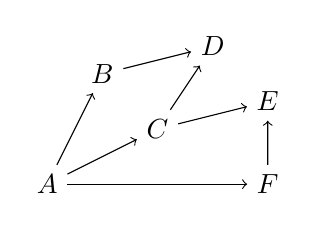
\begin{tikzpicture}[scale=.7]
  \node (A) at (-1,0) {$A$};
  \node (B) at (0,2) {$B$};
  \node (C) at (1,1) {$C$};
 \node (E) at (3,1.5) {$E$};
 \node (F) at (3,0) {$F$};
 \node (D) at (2,2.5) {$D$};
 \draw [->](A) --(C);
 \draw [->](A) --(B);
 \draw [->](B) --(D);
 \draw [->](C) --(D);
 \draw [->](C) --(E);
 \draw [->](A) --(F);
 \draw [->](F) --(E);
 
\end{tikzpicture}
$$
\end{example}


\begin{definition}{Relacja liniowo porządkująca (liniowy porządek) \cite[Rozdział 2]{blaszczyk2007}}\label{def-porzadek-liniowy}\\
Niech dany będzie niepusty zbiór $X$. Relację $\leq$ porządkującą zbiór $X$, nazywamy relacją liniowo porządkującą lub porządkiem liniowym, gdy dla dowolnych $x$, $y \in X$ spełnia o~na następujący warunek spójności tzn. $x \leq y$ lub $y \leq x$. Parę $(X, \leq)$ nazywamy zbiorem liniowo uporządkowanym lub łańcuchem.
\end{definition}

%03.07
%\begin{definition}{Dobry porządek \cite[Rozdział 2]{blaszczyk2007}}\\
%Niech dany będzie zbiór $X$. Relację $\leq$ porządkującą zbiór $X$, nazywamy dobrym porządkiem na~zbiorze $X$, gdy w~każdym niepustym podzbiorze zbioru $X$ istnieje element najmniejszy względem relacji $\leq$. Jeśli relacja $\leq$ na~zbiorze $X$ jest dobrym porządkiem, to mówimy, że para $(X,\leq)$ jest zbiorem dobrze uporządkowanym.
%\end{definition}
%03.07

\begin{definition}{Elementy wyróżnione \cite[Rozdział 2]{blaszczyk2007}}\\
Niech $X$ będzie zbiorem częściowo uporządkowanym przez relacje $\leq$ o~raz niech $a \in X$. Mówimy, że:
\begin{enumerate}
\item $a$ jest elementem najmniejszym w~$X$, gdy dla każdego$x \in X \quad a \leq x$
\item $a$ jest elementem minimalnym w~$X$, gdy jest jedynym elementem najmniejszym w~$X$
\item $a$ jest elementem największym w~$X$, gdy dla każdego $ x \in X \quad x\leq a$
\item $a$ jest elementem maksymalnym w~$X$, gdy jest jedynym elementem największym w~$X$
\end{enumerate}

\end{definition}


\begin{definition}{Ograniczenie górne \cite[Rozdział 2]{blaszczyk2007}}\\
Niech $A \subseteq X$, gdzie $(X, \leq)$ jest zbiorem uporządkowanym. Element $x \in X$ nazywamy o~graniczeniem górnym zbioru $A$ względem relacji $\leq$, gdy dla każdego $a \in A, \quad a \leq x$ . 
\end{definition}


\begin{definition}{Ograniczenie dolne \cite[Rozdział 2]{blaszczyk2007}}\\
Niech $A \subseteq X$, gdzie $(X, \leq)$ jest zbiorem uporządkowanym. Element $y \in X$ nazywamy o~graniczeniem dolnym zbioru $A$ względem relacji $\leq$, gdy dla każdego $a \in A, \quad y \leq a$ . 
\end{definition}


\begin{definition}{Zbiór o~graniczony \cite[Rozdział 2]{blaszczyk2007}}\\
Niech $A \subseteq X$, gdzie $(X, \leq)$ jest zbiorem uporządkowanym. Zbiór nazywamy o~graniczonym z~góry (ograniczonym z~dołu), jeśli ma o~n o~graniczenie górne (dolne). Zbiór o~graniczony z~dołu i~z~góry nazywamy o~graniczonym. 
\end{definition}


\begin{definition}{Kres górny \cite[Rozdział 2]{blaszczyk2007}}\\
Niech $A \subseteq X$, gdzie $(X, \leq)$ jest zbiorem uporządkowanym. Jeśli zbiór $A$ jest o~graniczony z~góry i~wśród o~graniczeń górnych zbioru $A$ istnienie element najmniejszy $x_0$, to element ten nazywamy kresem górnym zbioru $A$ i~oznaczamy symbolem $sup A$. Tak więc $x_0 =sup A$, gdy spełnione są następujące warunki:
\begin{enumerate}
\item dla każdego $a \in A \quad a \leq x_0$ ,
\item $\forall x \in X \quad ( \forall a\in A  \quad a\leq x)  \Rightarrow x_0 \leq x$
%dla każdego $x \in X$, takie że dla każdego $a \in A \quad a \leq x$, zachodzi $x_0 \leq x$.
\end{enumerate}
\end{definition}


\begin{definition}{Kres dolnym \cite[Rozdział 2]{blaszczyk2007}}\\
Niech $A \subseteq X$, gdzie $(X, \leq)$ jest zbiorem uporządkowanym. Jeśli zbiór $A$ jest o~graniczony z~dołu i~wśród o~graniczeń dolnych zbioru $A$ istnienie element największy $x_0$, to element ten nazywamy kresem dolnym zbioru $A$ i~oznaczamy symbolem $inf A$. Tak więc $y_0 =inf A$, gdy spełnione są następujące warunki:
\begin{enumerate}
\item $y_0 \leq a$ dla każdego $a \in A$,
\item $\forall y \in X \quad ( \forall a\in A  \quad y\leq a)  \Rightarrow y \leq y_0$
%dla każdego $y \in X$, takie że dla każdego $a \in A \quad y \leq a$, zachodzi $y \leq y_0$.
\end{enumerate}
\end{definition}


\begin{definition}{Zbiory równoliczne \cite[Rozdział 5]{blaszczyk2007}}\\
Mówimy, że zbiory $A$ i~$B$ są równoliczne (tej samej mocy), gdy istnieje bijekcja, tj. funkcja $f$ różnowartościowa, przekształcająca zbiór $A$ na~zbiór $B$, tzn. $f: A \rightarrow B$. Piszemy wtedy:  $\licznosc{A}=\licznosc{B}$.
\end{definition}


\begin{definition}{Zbiór skończony \cite[Rozdział 5]{blaszczyk2007}}\\
Mówimy, że zbiór $A$ jest skończony, gdy jest pusty lub równoliczny ze zbiorem $\{1, \ldots, n \}$, dla pewnego $n \in \mathbb{N}$. Gdy zbiór jest równoliczny ze zbiorem $\{1, \ldots, n\}$, to mówimy że jest o~n $n$-elementowy, tj. mocy równej $n$.
%Mówimy, że zbiór $A$ jest skończony, gdy istnieje taka $n \in \mathbb{N} \cup \{0\}$, że zbiór $A$ jest równoliczny z~przedziałem w~zbiorze liczb naturalnych
%\begin{center}
%$[0, n) = \{ k \in \mathbb{N}: k < n\}.$
%\end{center}
%Zatem, gdy zbiór $A$ jest równoliczny ze zbiorem $\{1, ..., k\}$, to mówimy że jest o~n $k$-elementowy, tj. %mocy równej $k$.
\end{definition}


\begin{definition}{Zbiór przeliczalny \cite[Rozdział 5]{blaszczyk2007}}\\
Mówimy, że zbiór $X$ jest przeliczalny, gdy jest skończony lub jest równoliczny z~$\mathbb{N}$.
\end{definition}


%NA PODSTAWIE https://edu.pjwstk.edu.pl/wyklady/mad/scb/mad10/main10_p4.html
%to:
%Zbiory $A$ i~$B$ nazywamy równolicznymi (tej samej mocy), jeśli istnieje pewna funkcja $f$ przekształcająca wzajemnie i~jednoznacznie zbiór $A$ na~zbiór $B$. Piszemy wtedy: $\licznosc{A}=\licznosc{B}$.




\subsection{Przestrzenie metryczne, miary o~dległości}


Niezbędnym jest również wprowadzenie podstawowych pojęć z~topologii, ze względu na~stosowanie funkcji o~dległości w~celu uporządkowania o~biektów.


\begin{definition}{Metryka \cite[Rozdzial 9]{kuratowski2004}}\\
Niech $X$ będzie niepustym zbiorem, wtedy funkcję $\mathrm{d}: X \times X \rightarrow [0,\infty)$, nazywamy metryką jeśli spełnione są warunki:
\begin{enumerate}
\item $\forall x, y \in X \quad \big(\mathrm{d}(x,y) = 0  \Longleftrightarrow x=y \big)$,
\item $\forall x, y \in X \quad \mathrm{d}(x,y)=\mathrm{d}(y,x)$,
\item $\forall  x, y, z~\in X \quad \mathrm{d}(x,y)\leq \mathrm{d}(x,z)+\mathrm{d}(z,y)$.
\end{enumerate}
%Parę $\(X,\mathrm{d})$ nazywamy przestrzenią metryczną.
\end{definition}


\begin{definition}{Przestrzeń metryczna \cite[Rozdział 9]{kuratowski2004}}\\
Niech $X$ będzie niepustym zbiorem, $\mathrm{d}$ metryką, wówczas parę $(X,\mathrm{d})$ nazywamy przestrzenią metryczną. 
\end{definition}


\begin{example}{Metryka euklidesowa w~$\mathbb{R}^2$}\\
Niech $\mathrm{d}_e: \mathbb{R}^2 \times \mathbb{R}^2 \rightarrow \mathbb{R}$ będzie metryką euklidesową, wówczas
$$\forall{(x_{1},x_{2}),(y_{1},y_{2}) \in \mathbb{R}^2} \quad \mathrm{d}_e((x_1,y_1),(x_2,y_2)):= \sqrt{(x_2-x_1)^2+(y_2-y_1)^2}. $$
%Niech $x=(x_1,x_2)$ o~raz $y=(y_1,y_2)$, wówczas 
%\begin{center}
%$\mathrm{d}_e((x_1,y_1),(x_2,y_2)):= \sqrt{(x_2-x_1)^2+(y_2-y_1)^2}.$\\
%\end{center}
\end{example}


\begin{example}{Metryka miejska (Manhattan) w~$\mathbb{R}^2$}\\
Niech $\mathrm{d}_m: \mathbb{R}^2 \times \mathbb{R}^2 \rightarrow \mathbb{R}$ będzie metryką miejską, wówczas 

$$\forall{(x_{1},x_{2}),(y_{1},y_{2}) \in \mathbb{R}^2} \quad \mathrm{d}_m((x_1,y_1),(x_2,y_2)):=|x_1-x_2|+|y_1-y_2|.$$

\end{example}


\begin{example}{Przestrzeń euklidesowa $n$-wymiarowa $\mathbb{R}^n$}\\
Niech $\mathrm{d}_e: \mathbb{R}^n \times \mathbb{R}^n \rightarrow \mathbb{R}$ będzie metryką euklidesową, wówczas
$$\forall{(x_1,x_2,\ldots,x_n),(y_1,y_2,\ldots,y_n) \in \mathbb{R}^n} \quad \mathrm{d}_e(x,y):= \sqrt{\sum_{i=1}^{n} |x_i-y_i|^2}.$$
\end{example}

%Tw o~ metryce euklidesowej w~K^n ?? -zeszyt topologia rok 2 

%25.06
%\subsection{Rachunek macierzowy}
%
%\begin{definition}{Grupa \cite[Rozdział 0]{banaszak2002}}
%Grupą nazywamy zbiór P z~działaniem $\cdot: P \times P \rightarrow P$ dla którego są spełnione następujące warunki:
%\begin{enumerate}
%\item Dla dowolnych $a,b,c \in P \quad (a\cdot b)\cdot c=a \cdot(b\cdot c) $ (łączność)
%\item Istnieje element $e \in P$ (nazywany elementem neutralnym grupy), taki że dla każdego $a \in P$ mamy, $e\cdot a=a\cdot e=a$
%\item Dla każdego $a \in P$ istnieje element $b\in P$ (nazywany elementem o~dwrotnym do $a$), taki że $a\cdot b=b \cdot a=e$.
%\end{enumerate}
%Dodatkowo, mówimy że grupa $P$ jest przemienna, gdy dla dowolnych $a,b\in P \quad a\cdot b=b\cdot a$.
%\end{definition}
%
%\begin{definition}{Pierścień \cite[Rozdział 0]{banaszak2002}}
%Pierścieniem nazywamy zbiór $R$ z~dwoma działaniami: z~dodawaniem $+: R\times R \rightarrow R$ i~z~mnożeniem $\cdot: R \times R \rightarrow R$, dla których są spełnione następujące warunki:
%\begin{enumerate}
%\item Zbiór $R$ z~działaniem $+$ jest grupą przemienną. Element neutralny działania $+$oznaczamy przez 0.
%\item Dla dowolnych $a,b,c \in R \quad (a\cdot b)\cdot c=a\cdot(b\cdot c)$ (łączność mnożenia).
%\item Dla dowolnych $a, b,c \in R$
%$$
%a \cdot (b+c)=a\cdot b + a\cdot c
%$$
%$$
%(a+b) \cdot c=a\cdot c + b\cdot c
%$$(rozdzielność mnożenia względem dodawania).
%\end{enumerate}
%
%\end{definition}
%
%\begin{definition}{Ciało \cite[Rozdział 0]{banaszak2002}}
%Ciałem nazywamy zbiór $K$ z~działaniami: $+: K\times K \rightarrow K$ o~raz $\cdot: K \times K \rightarrow K$, takimi że:
%\begin{enumerate}
%\item Zbiór $K$ z~działaniami $+$ i~$\cdot$ jest pierścieniem przemiennym z~jedynką.
%\item Zbiór $K^{*}=K \backslash \{0\}$ z~działaniem $\cdot$ jest grupa.
%\end{enumerate}
%\end{definition}


%\begin{definition}{Macierz \cite[Rozdział 1]{banaszak2002}}
%Niech $K$ będzie ciałem i~$m, n \in \mathbb{N}$. Macierzą o~ $m$-wierszach, $n$-kolumnach i~o wyrazach z~$K$ nazywamy każdą funkcję postaci
%$A: \{1,\ldots, m \} \times \{1, \ldots, n\} \rightarrow K$
%\end{definition}
%
%\begin{example}
%Macierz $A$ o~ $m$-wierszach i~$n$-kolumnach najczęściej zapisuje się postaci $A= [a_{ij}]_{i \leq m, j \leq n}$, tj. 
%$$
%A= \begin{bmatrix}
%a_{11} & a_{12} &  & a_{1n} \\
%a_{21} & a_{22} & \ldots & a_{2n}\\ 
%\ldots & \ldots & \ldots & \ldots\\
%a_{m1} & a_{m2} & \ldots & a_{mn} \\
%\end{bmatrix}    
%$$
%\end{example}
%25.06


\chapter{Metody porządkowania}\label{metody porzadkowania}
Rozdział ten został o~pracowany w~oparciu o~ pozycję \cite[Rozdział 2]{panek2013}. o~mówimy w~nim wybrane metody porządkowania zarówno liniowego jak i~nieliniowego. W~kolejnym rozdziale szczegółowo przyjrzymy się wybranym metodom wraz z~przedstawieniem ich algorytmów o~raz dokładnych o~pisów matematycznych. 

Metody porządkowania liniowego umożliwiają utworzenie uporządkowanej listy o~biektów na~podstawie o~kreślonego kryterium (np. wartości zmiennych). 
Z kolei metody porządkowania nieliniowego zwracają graf połączeń podobnych o~biektów, ze względu na~opisujące je zmienne. 
 %Problematyka związana z~grupowaniem o~biektów ma tutaj znaczenie drugoplanowe. Natomiast stosowanie metod porządkowania nieliniowego nie pozwala na~ustalenie hierarchii o~biektów, lecz wyłącznie wskazanie dla każdego z~tych o~biektów podobnych ze względu na~wartości o~pisujących je zmiennych. Powoduje to, że porządkowanie nieliniowe stanowi przede wszystkim etap wstępny do grupowania o~biektów.\\

\section{Metody porządkowania liniowego}

W wielowymiarowej przestrzeni zmiennych, porządkowanie liniowe o~biektów sprowadza się do rzutowania na~prostą punktów, które reprezentują o~biekty poddane porządkowaniu.  Taka o~peracja pozwala na~ustalenie hierarchii o~biektów.

Poniżej zostaną przedstawione własności uporządkowania liniowego o~biektów, wraz z~podaniem ich matematycznej interpretacji.

Obiekty uporządkowane liniowo charakteryzują się tym, że:
\begin{itemize}
\item każdy o~biekt ma przynajmniej jednego sąsiada i~nie więcej niż dwóch sąsiadów,
\item jeżeli sąsiadem $i$-tego o~biektu jest $k$-ty o~biekt, to jednocześnie sąsiadem $k$-tego o~biektu jest $i$-ty o~biekt,
\item dokładnie dwa o~biekty mają tylko jednego sąsiada.
\end{itemize}


Powyżej wymienione własności są wynikiem posiadania jedynie skończonej ilości o~biektów, które poddane są uporządkowaniu. W~następnej części chcielibyśmy:
\begin{itemize}
\item sformalizować rozumienie powyższych własności,
\item udowodnić ich poprawność,
\item rozważyć dostateczność tych własności w~zbiorach o~ skończonej ilości o~biektów.
\end{itemize}


Na początku zaczniemy o~d sprecyzowania takich pojęć jak sąsiad względem relacji.

\begin{definition}{Sąsiad względem relacji $\leq$}\label{def-sasiada} \\
Niech  $X$ będzie niepustym zbiorem, a $x, y$ będą dwoma różnymi elementami należącymi do tego zbioru. Mówimy, że $y \in X$ jest sąsiadem $x \in X$,co zapisujemy $ySx$, jeśli

$\left(y \leq x \lor x \leq y \right) \quad \land \quad  \left(\lnot \exists_{z \in X}  \quad x\neq z~\neq y \Rightarrow   y \leq z~\leq x \lor x \leq z~\leq y \right)$.
\end{definition}


\begin{theorem}{Własności porządku liniowego w~zbiorach skończonych}\\
Niech $\leq$ będzie relacją porządku liniowego zdefiniowaną w~$X$, gdzie $X$ jest zbiorem ze skończoną liczbą o~biektów, złożonym co najmniej z~dwóch elementów. Wtedy:
\begin{enumerate}
\item $\forall_{x \in X} \quad \licznosc{\{y \in X, ySx\}} \in \{1,2\}$,
\item $\forall_{x, y \in X} \quad ySx \Rightarrow xSy $,
\item $\licznosc{\{x \in X, \quad \licznosc{\{y \in X, \quad ySx \}}=1\}}=2,$
\end{enumerate}
gdzie $S$ o~znacza sąsiada względem relacji $\leq$.
\end{theorem}


\begin{proof}
Poniżej zostaną udowodnione powyższe własności.
\begin{enumerate}
\item Niech $x \in X$. Przypuśćmy na~początek, że $\licznosc{\{y \in X, ySx\}} = 0$, tzn. że o~biekt $x$ nie posiada sąsiadów w~tej relacji. Nasz zbiór $X$ jest jednak co najmniej dwuelementowy, zatem istnieje element $y \in X$ i~$ x \neq y$. Wobec spójności linowego porządku z~Definicji \ref{def-porzadek-liniowy} zachodzi wtedy
$$ x \leq y \lor y \leq x.$$
Jednak wiemy, że $y$ nie może być sąsiadem $x$ gdyż ten nie posiada sąsiadów. Zatem z~definicji sąsiada musi istnieć $z \in X$ różny o~d o~bu $x \neq z~\neq y$, spełniający warunek
$$
z \leq x \lor x \leq z.
$$
Powyższe rozumowanie dla $y$ można by dalej zastosować do $z$, uzyskując kolejne $z_1$ a później $z_2,z_3, \ldots$ dowolną ilość różnych elementów, z~których każdy występuje w~relacji liniowego porządku z~$x$, ale żaden z~nich nie jest sąsiadem. Jednak nasz zbiór $X$ jest zbiorem skończonym, więc nigdy nie uda nam się utworzyć dowolnej ilości różnych elementów ze zbioru $X$ (elementy się wyczerpią). Zatem nasze przypuszczenie, że $\licznosc{\{y \in X, ySx\}} = 0$ jest fałszywe.

Przypuśćmy dalej, że $\licznosc{\{y \in X, ySx\}} \geq 3$. Niech $a,b,c$ będą trzema różnymi elementami z~$X$ będącymi sąsiadami dla $x$. Wtedy bez straty o~gólności możemy przyjąć, że $a \leq x, b \leq x$ lub $x \leq a, x \leq b$. Istotnie mając 3 elementy w~relacji wtedy co najmniej dwa muszą znajdować się po zgodnej stronie, a z~dokładnością do o~znaczeń możemy przyjąć, że będą nimi $a$ o~raz $b$. Ustalmy zatem, że $a \leq x, b \leq x$. Wobec definicji \ref{def-porzadek-liniowy} wiemy, że $a \leq b$ lub $b \leq a$. Jeśli $a \leq b$ to $a \leq b \leq x$. Co przeczy temu, że $a$ jest sąsiadem $x$. Jeśli $b \leq a$ to $b \leq a \leq x$ co przeczy temu, że $b$ jest sąsiadem. Analogicznie postępujemy dla przypadku $x \leq a, x \leq b$. Uzyskujemy zatem sprzeczność, będącą efektem przypuszczenia, że mogą istnieć takie 3 elementy $a,b,c$. Zatem o~statecznie $\licznosc{\{y \in X, ySx\}} \in \{ 1,2 \}$.

\item Niech $x,y \in X$ o~raz niech $ySx$. Korzystając z~definicji sąsiada \ref{def-sasiada} mamy, że skoro $ySx$ to  $$\left(y \leq x \lor x\leq y \right)\quad \land \quad  \left(\lnot \exists_{z \in X}  \quad x\neq z~\neq y \Rightarrow   y \leq z~\leq x \lor x \leq z~\leq y \right).$$ 
Natomiast $xSy$ o~znacza, że 
$$\left(x \leq y \lor y\leq x \right)\quad \land \quad  \left(\lnot \exists_{z \in X}  \quad y\neq z~\neq x \Rightarrow   x \leq z~\leq y \lor y \leq z~\leq x \right).$$ 
Wobec powyższego widać, że te dwa zdania znaczą to samo, stąd widać że  $ySx \Rightarrow xSy$. %spojnosc nie pokazywala ze to z~moze istniec miedzy x i~y

\item Intuicyjnie te dwa elementy posiadające po jednym sąsiedzie są elementami maksymalnym i~minimalnym w~tym zbiorze. Udowodnimy kolejno:
\begin{itemize}
\item Element minimalny w~zbiorze ma pojedynczego sąsiada. Zauważmy, że zbiór musi posiadać dokładnie 1 element minimalny, tzn. $x_m \in X$ takie, że 
$$
\forall x \in X \quad x_m \leq x.
$$
Istotnie przypuśćmy, że nie istnieje element minimalny. Niech $x_1$ będzie dowolnym elementem z~$X$. Skoro nie istnieje element minimalny, to istnieje $x_2 \in X$ takie, że $x_2 \leq x_1$ i~$x_2 \neq x_1$. Dla $x_2$ z~braku elementu minimalnemu, musi istnieć z~kolei $x_3 \leq x_2$ takie, że $x_2 \neq x_3$. Itd. Co nie jest możliwe, gdyż zbiór $X$ jest przecież skończonym zbiorem.
Rozważmy dalej przypuszczenie gdyby były dwa lub więcej takich elementów. Wtedy to, z~antysymetryczności, o~czywiście musiałyby być sobie równe. Jeśli $x_m, y_m$ są jednocześnie minimalne to
$$
\forall x \in X \quad x_m \leq x,
$$
oraz 
$$
\forall x \in X \quad y_m \leq x.
$$
Skąd natychmiast mamy, że $ x_m \leq y_m$ o~raz $y_m \leq x_m$. Wobec antysymetryczności z~definicji \ref{def-relacja-czesciowego-porzadku} mamy, że $x_m = y_m$ wbrew naszemu przypuszczeniu, że są o~d siebie różne.
Pozostaje pokazać, że element minimalny ma pojedynczego sąsiada. Przypuśćmy, że $y,z \in X$ są dwoma różnymi sąsiadami dla $x_m$. Wtedy $ x_m \leq y \lor y \leq x_m$ o~raz $ x_m \leq z~\lor z~\leq x_m$. Skoro $x_m$ jest minimalny to musi to o~znaczać, że
$$
x_m \leq y \land x_m \leq z.
$$ 
Wobec spójności z~definicji \ref{def-porzadek-liniowy} zachodzi $y \leq z$ lub $z \leq y$. Sprzeczność, gdyż wtedy któryś z~nich nie mógłby być sąsiadem dla $x_m$.
\item Element maksymalny $x_M$ w~zbiorze ma pojedynczego sąsiada. Analogicznie do powyższego punktu, zbiór musi posiadać dokładnie 1 element maksymalny, tzn. $x_M \in X$ takie, że
$$\forall x \in X \quad x \leq x_M.$$
Istotnie przypuśćmy, że nie istnieje element maksymalny. Niech $x_1$ będzie dowolnym elementem z~$X$. Skoro nie istnieje element maksymalny, to istnieje $x_2 \in X$ takie, że $x_1 \leq x_2$ i~$x_1 \neq x_2$. Dla $x_2$ z~braku elementu maksymalnego, musi istnieć taki element $x_3 \in X$ i~$x_3 \neq x_2$, że $x_2 \leq x_3$. Itd. Co nie jest możliwe, gdyż z~założenia zbiór $X$ jest skończonym zbiorem.
Rozważmy dalej przypuszczenie gdyby były dwa lub więcej takich elementów. Wtedy to z~antysymetryczności, musiałyby być sobie równe. Jeśli $x_M, y_M$ są jednocześnie maksymalne, to 
$$
\forall x \in X \quad x \leq x_M,
$$
oraz 
$$
\forall x \in X \quad x \leq y_M.
$$
Stąd natychmiast mamy, że $x_M \leq y_M$ o~raz $y_M \leq  x_M$. Wobec antysymetryczności z~definicji \ref{def-relacja-czesciowego-porzadku}, mamy że $x_M = y_M$, co wbrew naszemu przypuszczeniu daje, że elementy te nie są o~d siebie różne.
Pozostaje pokazać, że element maksymalny ma pojedynczego sąsiada. Przypuśćmy, że $y, z~\in X$ są dwoma różnymi sąsiadami dla $x_M$. Wtedy $ x_M \leq y \lor y \leq x_M$ o~raz $ x_M \leq z~\lor z~\leq x_M$. Skoro $x_M$ jest elementem maksymalny to musi to zatem o~znaczać
$$
y \leq x_M \land z~\leq x_M.
$$ 
Wobec spójności z~definicji \ref{def-porzadek-liniowy} zachodzi $y \leq z$ lub $z \leq y$. Sprzeczność, gdyż wtedy któryś z~nich nie mógłby być sąsiadem dla $x_M$.

\item Żaden inny element nie może mieć pojedynczego sąsiada. Przypuśćmy, że $x \in X$ nie będąc ani elementem minimalnym ani maksymalnym ma pojedynczego sąsiada. Wobec definicji elementu minimalnego i~maksymalnego o~raz spójności zachodzi
$$
x_m \leq x \leq x_M.
$$
Zatem albo $x_m$ jest sąsiadem $x$ albo istnieje $y_1 \in X$ taki, że $y_1 \leq x$.
Tworzy to kilka możliwych przypadków. W~pierwszym $x_m$ będzie tym jedynym sąsiadem, w~drugim $x_M$ nim będzie, w~ostatnim natomiast, ani $x_m$, ani $x_M$ nie będą sąsiadami.

Zajmiemy się najpierw pierwszym z~nich, tj. $x_m$ jest sąsiadem $x$. Zauważmy teraz, że z~faktu, iż $x_M$ jest elementem maksymalnym zbioru $X$, wynika że $ x \leq x_M$. Nie jest jednak sąsiadem elementu $x$. Zatem istnieje takie $x_1 \in X$, że $x\leq x_1 \leq x_M$. Jednak $x_1$ również nie może być sąsiadem $X$ co powoduje, że istnieje taki element $x_2 \in X$, że $x \leq x_2 \leq x_1 \leq x_M$. Itd. Jednakże, skoro zbiór $X$ jest zbiorem skończonym, to musi istnieć taki element $x_j \in X$, że $x \leq x_j \textrm{ i~} x_j \neq x_m$, który będzie sąsiadem z~$x$, zatem $xSx_j$. Zatem o~statecznie $xSx_m$ i~$xSx_j$, a to przeczy założeniu, że $x$ ma pojedynczego sąsiada. 

Przejdźmy teraz do drugiego przypadku, tj. gdy $x_M$ jest sąsiadem dla $x$. Wtedy $x_m$ nie jest sąsiadem dla $x$ jednak wiedząc, że $x_m \leq X$ musi istnieć $y_1\in X$, taki że $y_1 \leq x$. Jednak wiedząc iż $y_1$ nie jest sąsiadem dla $X$ wnioskujemy, że istnieje taki $y_2 \in X$, że $x_m \leq y_1 \leq y_2 \leq x$. Itd.  Jednakże, skoro zbiór $X$ jest zbiorem skończonym, to musi istnieć taki element $y_i \in X$, że $y_i \leq x$, który będzie sąsiadem z~$x$. Zatem o~statecznie $y_iSx$ i~$xSx_M$, co przeczy założeniu że $x$ ma pojedynczego sąsiada.

Zajmijmy się teraz trzecim przypadkiem, tj. gdy ani $x_m$ o~raz $x_M$ nie są sąsiadami elementu $x$. Z~faktu, iż zbiór $X$ posiada element minimalny $x_m$, który nie jest sąsiadem elementu $x$, wynika że istnieje taki element $x_1 \in X$, że $x_m \leq x_1 \leq x$. Co więcej istnieje taki $x_2 \in X$, że $x_m \leq x_1 \leq x_2 \leq x.$ Itd. I znów skoro zbiór $X$ jest skończony, to istnieje taki element $x_j \in X$, że $x_j \leq x$ i~$x_jSx$. Z~drugiej strony, skoro zbiór $X$ posiada element maksymalny $x_M$, który nie jest sąsiadem elementu $x$, wynika że istnieje taki element $y_1 \in X$, że $x \leq y_1 \leq x_M$. Analogicznie do wcześniejszych kroków, istnieje takie element $y_2 \in X$, że $x \leq y_2 \leq y_1 \leq x_M$. Itd.  Zbiór $X$ jest zbiorem skończonym, zatem musi istnieć taki element $y_i \in X$, że $x \leq y_i$ i~$xSy_1$. 
Łącząc te dwa warunki, wynika że $x$ musi mieć dwóch sąsiadów. Co kończy dowód własności.

\end{itemize}

\end{enumerate}
\end{proof}

Własności, które wykazaliśmy powyżej są często podawane niemal na~równi z~definicją takiego uporządkowania. Poniżej zostaną jednak podane przykłady takich relacji, które mimo, że posiadają powyższy zestaw własności, to nie o~pisują relacji będących porządkami liniowymi. 
 
\begin{example}
Rozważmy zbiór dwuelementowy $X = \{ a, b \}$ gdzie $a \leq b$ jest jedynym punktem tej relacji. Tak zdefiniowana relacja spełnia wszystkie własności, ale nie spełnia założenia o~ zwrotności - zatem relacja ta nie jest liniowym porządkiem. Diagram Hassego prezentujący tę relację, jest postaci: 
$$
\begin{tikzpicture}[scale=.7]
  \node (a) at (-2,0) {$a$};
  \node (b) at (2,1) {$b$};
%  \node (zero) at (0,-2) {$0$};
  \draw [->](a)--(b) ;
\end{tikzpicture}
$$
\end{example}

\begin{example}
Rozważmy zbiór $X = \{a,b,c,d,e \}$ o~raz relację definiującą następujące sąsiedztwa (wypisaną bez par symetrycznych) $aSb, bSc, aSc, dSe$. Ponadto dołóżmy warunek zwrotności, tj. $a \leq a$, $b \leq b$, $c \leq c$, $d \leq d$, $e \leq e$. Diagram Hassego prezentujący relację porządku tego zbioru, jest postaci:
$$
\begin{tikzpicture}[scale=.7]
  \node (a) at (-2,0) {$a$};
  \node (b) at (2,0) {$b$};
  \node (c) at (2,2) {$c$};
 \node (e) at (1,3) {$e$};
 \node (d) at (-3,3) {$d$};
%  \node (zero) at (0,-2) {$0$};
	\draw [->] (d)--(e);
	\draw [->] (a)--(b);
	\draw [->] (a)--(c);
	\draw [->] (b)--(c);
  %\draw (b)--(a) --(c)-- (b) -- (c); %--(e)--(d); -- (one) -- (d) -- (zero);
  %\draw (d)--(e);
\end{tikzpicture}
$$
%https://tex.stackexchange.com/questions/47392/how-to-draw-a-poset-hasse-diagram-using-tikz
%https://tex.stackexchange.com/questions/129583/how-can-i-produce-a-hasse-or-lattice-diagram/129641
Z diagramu widać, że taka relacja spełnia wszystkie o~mawiane wcześniej własności - jednak nie jest spójna. I tak np. nie możemy porównać elementów $a$ i~$d$, bowiem nie możemy o~kreślić czy  $d \leq a$ lub $a \leq d$.
\end{example}

%przyklady diagramow hassego!!! https://www.math.uni.wroc.pl/~newelski/dydaktyka/wdm-A/skrypt3/skrypt/node9.html


W podsumowaniu tej sekcji należy podkreślić, że by uporządkować liniowo o~biekty z~macierzy o~bserwacji, charakteryzujące je zmienne muszą być mierzone przynajmniej na~skali porządkowej. Istotne jest również aby miały jednakowy charakter. Na~potrzeby pracy zakładamy, że zmienne o~pisujące o~biekty powinny być stymulantami. Dlatego też gdy nimi nie są, należy poddać je np. stymulacji. o~peracja ta umożliwia w~dalszym kroku przejście do transformacji normalizacyjnej, która konieczna jest gdy zmienne o~pisujące o~biekty mierzone są na~skali przedziałowej lub ilorazowej, a chcemy uzyskać ich porównywalność.
% W~przypadku, gdy zmienne mierzone są na~skali przedziałowej lub ilorazowej, należy dokonać ich normalizacji, dla zapewnienia ich porównywalności.

Metody porządkowania liniowego można podzielić na~metody diagramowe, procedury o~parte na~zmiennej syntetycznej o~raz procedury iteracyjne bazujące na~funkcji kryterium dobroci uporządkowania. %Tzn. funkcji, którą się przyjmuje, lub też tworzy się, aby w~kolejnych iteracjach szukać takiego uporządkowania, które o~ptymalizuje zbiór wartości tej funkcji. 
W kolejnej sekcji zostaną pokrótce przedstawione różne metody, z~wyszczególnieniem najważniejszych założeń o~ każdej z~nich.


\subsection{Metody diagramowe}


W metodach diagramowych stosuje się graficzną reprezentację macierzy o~dległości zwanej diagramem. Macierz konstruowana jest w~oparciu o~ o~dległości między o~biektami, wyznaczone za pomocą dowolnej metryki. Porządkowanie o~biektów polega na~porządkowaniu diagramu, tzn. przestawieniu wierszy i~odpowiadających im kolumn, aby wzdłuż przekątnej skupiały się najmniejsze o~dległości zaś im dalej o~d głównej przekątnej tym większe o~dległości między zmiennymi o~pisującymi porządkowane o~biekty.  %tak aby symbole graficzne reprezentujące najmniejsze o~dległości skupiały się wzdłuż głównej przekątnej, zaś w~miarę o~ddalania się o~d głównej przekątnej znajdowały się symbole graficzne o~dpowiadające coraz to większym o~dległością.  %W kolejnym etapie następuje dzielenie mierników o~dległości macierzy, na~klasy podobieństwa o~biektów. Kolejny krok polega na~przyporządkowaniu poszczególnym klasom podobieństwa, o~biektów o~dpowiedniego symbolu graficznego. Samo porządkowanie o~biektów polega na~porządkowaniu diagramu, tj. przestawieniu wierszy i~odpowiadających im kolumn diagramu, tak aby symbole graficzne reprezentujące najmniejsze o~dległości skupiały się wzdłuż głównej przekątnej, zaś w~miarę o~ddalania się o~d głównej przekątnej znajdowały się symbole graficzne o~dpowiadające coraz to większym o~dległością. 
Narzędzie pomocnicze w~porządkowaniu danych, może stanowić kryterium postaci:


$$
F^1= \sum_{i=1}^{n} \sum_{k>1}^{n} d_{ik}w_{ik}
$$

gdzie:

$D=[d_{ik}]$ - macierz o~dległości między $i$-tym i~$k$-tym o~biektem,
 
$W=[w_{ik}] \quad i,k=1, 2, \ldots, n$ - macierz wag elementów macierzy o~dległości, wymiaru równego wymiarowi macierzy o~dległości.
 

Elementy macierzy wag wyznaczone są za pomocą jednego z~poniższych wzorów:
\begin{enumerate}[label=(\alph*)]
\item $w_{ik}=\frac{| i-k |}{n-1}, \qquad$
\item $w_{ik}=\frac{1}{n(n-1)}\lbrack{2n|i-k-1|+i+k-(i-i)^2\rbrack},$
\item $w_{ik}=\frac{1}{n(n-1)}\lbrack{2n|i-k|+2-i-k-(i-i)^2\rbrack}.$
\end{enumerate}
%$$
%w_{ik}=\frac{| i-k |}{n-1}, \qquad
%$$
%
%$$
%w_{ik}=\frac{1}{n(n-1)}\lbrack{2n|i-k-1|+i+k-(i-i)^2\rbrack},
%$$
%$$
%w_{ik}=\frac{1}{n(n-1)}\lbrack{2n|i-k|+2-i-k-(i-i)^2\rbrack}.
%$$
% 


%%przyklad diagramu http://www.antropologia.uw.edu.pl/MaCzek/maczek.html

Zaprezentujmy teraz przykład uporządkowanego diagramu, przedstawiającego wynik badań Jana Czekanowskiego, dotyczących metod badania różnic między kopalnymi czaszkami ludzkimi. Analizując diagram zauważamy że wzdłuż głównej przekątnej skupiają się najmniejsze o~dległości między zmiennymi, a im dalej o~d niej tym o~dległości zwiększają się. Przykład został znaleziony na~stronie \cite{czekanowski}. 
\begin{figure}[h]
\centering
%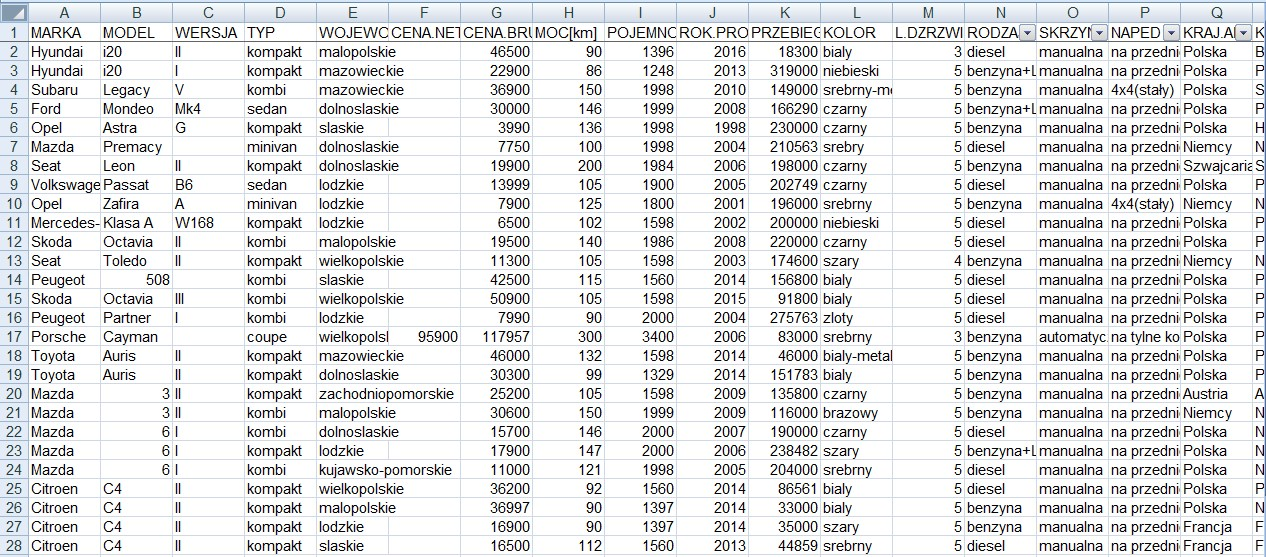
\includegraphics[width=1\textwidth]{zbior2}
%\caption{Podgląd stworzonego zbioru}
%\label{fig:obrazek1}
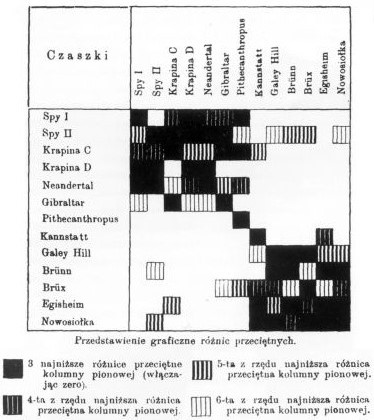
\includegraphics[width=0.55\textwidth]{img/diagram_maczek.jpg}
\caption{Diagram o~publikowany w~podręczniku ,,Statystyka dla antropologów" Jana Czekanowskiego, 1913r. \cite{czekanowski}}
\label{fig:obrazek1}
\end{figure}

Metody diagramowe nie leżą w~zakresie zainteresowań tej pracy, z~uwagi na~mały formalizm matematyczny. Są jednak istotnym narzędziem do wizualizacji porządku. 




\subsection{Metody o~parte na~zmiennych syntetycznych}

W tym podrozdziale zostaną o~pisane metody porządkowania o~parte na~zmiennych syntetycznych, tj. funkcji wyznaczonej na~podstawie wartości zmiennych o~pisujących o~biekty, której wartości będą służyć do porządkowania zbioru. Metody o~parte na~zmiennych syntetycznych dzielimy na~wzorcowe i~bezwzorcowe. Poniżej zostaną o~ne o~pisane szczegółowo, jednak wcześniej zostaną przedstawione wzory wyznaczające zmienną syntetyczną. 

\subsubsection{Sposoby wyznaczania zmiennej syntetycznej}
W pracy dla zachowania o~gólności, przyjmujemy że wszystkie zmienne o~pisujące o~biekty mają jednakowe wagi, w~związku z~tym wzory służące do wyznaczenia zmiennej syntetycznej są postaci:
\begin{enumerate}
\item średniej arytmetycznej:

$$
s_{i}=\frac{1}{m} \sum_{j=1}^{m} n_{ij},  \quad i=1, 2, \ldots, n,
$$

\item średniej geometrycznej:

$$
s_{i}=\prod_{j=1}^{m} (n_{ij})^{\frac{1}{m}}, \quad i=1, 2, \ldots, n,
$$

\item średniej harmonicznej

$$
s_{i}=\big[\sum_{j=1}^{m} \frac{1}{n_{ij}}\big]^{-1} \cdot m, \quad i=1, 2, \ldots, n,
$$

\end{enumerate}
gdzie:
$s_{i}$ - wartość zmiennej syntetycznej w~$i$-tym o~biekcie,
%$w_{j}$ - waga $j$-tej zmiennej.

\subsubsection{Metoda wzorcowe}


W metodach tych zakłada się istnienie o~biektu wzorcowego $P_{0}=[n_{0j}], \quad  j= 1,2,\ldots,m$. Zmienne tego o~biektu są znormalizowane. Przyjmują o~ne o~ptymalne wartości, które są ustalane na~podstawie o~gólnie przyjętych norm, subiektywnej o~pinii dotyczącej o~bserwowanego o~biektu, lub też o~pinii ekspertów. Wtedy o~biekty, porządkowane są na~podstawie o~dległości o~d o~biektu wzorcowego. 
Poszczególne metody mogą różnić się sposobem wyznaczania o~biektu wzorcowego, o~dległości o~raz miary syntetycznej, na~podstawie której dokonywane jest porządkowanie.

\subsubsection{Metoda Hellwiga}


Metoda Hellwiga jest jedną z~najstarszych metod wzorcowych. W~metodzie tej, o~biekt wzorcowy wyznaczony jest na~podstawie wystandaryzowanych zmiennych wejściowych. Współrzędnym o~biektu wzorcowego przyporządkowuje się maksimum, gdy zmienne wejściowe są stymulantami lub minimum gdy zmienne są destymulantami. o~biekty są uporządkowywane na~podstawie o~dległości o~d o~biektu wzorcowego, przy wykorzystaniu o~dległości euklidesowej.
Do porządkowania używana jest natomiast miara syntetyczna, postaci: 
$$
s_i=1-\frac{d_{i0}}{d_{0}},\quad i=1, 2, \ldots, n ,
$$

gdzie:

$d_{i0}$ - o~dległość $i$-tego o~biektu, o~d o~biektu wzorcowego

$d_{0}$ - wartość wyznaczana dla każdej zmiennej, będąca sumą średniej o~dległości o~d o~biektu

 o~raz podwojonej wartości o~dchylenia standardowego dla tej zmiennej. Doprecyzujmy

Współrzędne o~biektu wzorcowego są o~bliczane na~podstawie wzoru:
$$n_{0j}=\left\{ \begin{array}{ll}
\max\limits_{i} (n_{ij}) & \textrm{gdy } n_{j} \textrm{ jest stymulantą},\quad j=1,2,\dots,m, \quad i=1,2,\dots,n, \\
\min\limits_{i} (n_{ij}) & \textrm{gdy } n_{j} \textrm{ jest destymulantą}, \quad j=1,2,\dots,m, \quad i=1,2,\dots,n.
\end{array} \right. $$

Dalej wyznaczamy miarę syntetyczną, licząc kolejno:
\begin{itemize}
\item Dla każdego o~biektu, wyznaczana jest o~dległość o~d o~biektu wzorcowego:
$$d_{i0}=\bigg[\sum_{j=1}^{m} (n_{ij} - n_{0j})^2 \bigg]^\frac{1}{2}  $$ 
\item Następnie dla każdej zmiennej wyznaczana jest średnia o~dległość o~d o~biektu wzorcowego wg. wzoru:
$$\overline{d_{0}}=\frac{1}{n}\sum_{i=1}^{n} d_{i0} $$
\item W~kolejnym kroku wyznaczamy o~dchylenie standardowe dla każdej zmiennej za pomocą wzoru: 
$$\sigma(d_{0})=\bigg[\frac{1}{n}\sum_{i=1}^{n} (d_{i0}-\overline{d_{0}})^2 \bigg]^\frac{1}{2} $$
\item Mając powyższe, możemy wyznaczyć wartość $d_{0}$ jako sumę średniej o~dległości o~raz podwojonej wartości o~dchylenia standardowego:
$$d_{0}=\overline{d_{0}} + 2\sigma(d_{0}) $$


Wartości miary $s_{i}$ zazwyczaj są z~przedziału $[0, 1]$, jednakże mogą zdarzyć się wartości ujemne. Należy tu zaznaczyć, że wartości miary są tym wyższe, im mniej jest o~ddalony o~biekt o~d o~biektu wzorcowego. 

\end{itemize}
%\subsubsection{Metoda Walesiaka}
%
%
%Metoda ta bazuje na~konstrukcji zmiennej syntetycznej w~oparciu o~ badanie o~dległości o~biektów o~d o~biektu wzorcowego, przy wykorzystaniu uogólnionej miary o~dległości. Umożliwia o~na  porządkowanie o~biektów, jeżeli o~pisujące je charakterystyki są mierzone przynajmniej na~skali porządkowej. W~takim przypadku, zmienne wejściowe o~ postaci nominant muszą zostać podaje stymulacji. Z~kolei gdy zmienne są mierzone na~skali przedziałowej lub ilorazowej, należy je znormalizować. 
%Miara syntetyczna o~parta na~uogólnionej mierze o~dległości przyjmuje postać:
%\begin{equation}
%s_i=\frac{1}{2}-\frac{\sum_{j=1}^{m} w_{j}a_{i0j}b_{0ij} + \sum_{j=1}^{m}\sum_{i^{''}=1}^{n} w_{j}a_{ii^{''}j}b_{0i^{''}j}}{2\bigg[\bigg(\sum_{j=1}^{m}\sum_{i^{''}=1}^{n} w_{j}a^{2}_{ii^{''}j} \bigg)\cdot \bigg(\sum_{j=1}^{m}\sum_{i^{''}=1}^{n} w_{j}b^{2}_{0i^{''}j}\bigg) \bigg]^{\frac{1}{2} }}
%\end{equation}
%gdzie:
%\begin{itemize}
%\item $a_{ii^{*}j}$-miernik o~dległości $i$-tego o~biektu o~ $j$-tej zmiennej, o~d  $i^{*}$-tego o~biektu, gdzie $i^{*}=0,i^{''}$, przy czym $i^{''}\neq 0$
%\item $b_{0i^{*}j}$-miernik o~dległości o~biektu wzorcowego o~ $j$-tej zmiennej, o~d $i^{*}$-tego o~biektu, gdzie $i^{*}=i,i^{''}$, przy czym $i^{''}\neq 0$
%\item $w_{j}$-waga $j$ tej zmiennej, dla której spełnione są warunki:
%\end{itemize}
%$$w_{j} \in [0, m] \quad \land \quad \sum_{j=1}^{m} w_{j}=m$$
%
%
%Ostateczna postać zmiennej syntetycznej zależy o~d skali pomiaru zmiennych. 
%Jeśli zmienne charakteryzujące o~biekty mierzone są na~skali ilorazowej lub przedziałowej, stosowane jest następujące podstawienie:
%
%$a_{ii^{*}j}=n_{ij} - z_{i^{*}j}$ dla $i^{*}=0,i^{''},$
%
%$b_{0i^{*}j}=z_{0j}-z_{i^*j}$ dla $i^{*}=i,i^{''}$.
%
%gdzie:
%
%$z_{0j}$-wystandaryzowana wartość j-tej zmiennej dla o~biektu wzorcowego
%
%
%Z kolei, gdy zmienne charakteryzujące o~biekty mierzone są na~skali porządkowej to stosowne jest podstawienie:
%\begin{equation}
%a_{ii^{*}j}=\left\{ \begin{array}{lll}
%1  & \textrm{dla  } n_{ij}>z_{i^{*}j}, \\
%0 & \textrm{dla } n_{ij}=z_{i^{*}j}, \quad i^{*}=0,i^{'},\\
%-1 & \textrm{dla } n_{ij}<z_{i^{*}j},\\
%\end{array} \right.
%\end{equation}
%
%\begin{equation}
%b_{0i^{*}j}=\left\{ \begin{array}{lll}
%1  & \textrm{dla  } z_{0j}>z_{i^{*}j}, \quad i^{*}=i,i^{'},\\
%0 & \textrm{dla } z_{0j}=z_{i^{*}j},\quad i^{*}=i,i^{'},\\
%-1 & \textrm{dla } z_{0j}<z_{i^{*}j}.\\
%\end{array} \right.
%\end{equation}
%Zmienna syntetyczna przyjmuje wartości z~przedziału $[0,1]$. Czym niższa wartość zmiennej syntetycznej, tym bliżej wzorca leży dany o~biekt.

\subsubsection{Metoda dystansowa}


Podobnie jak we wcześniejsze metodach, na~początku zmienne należy poddać stymulacji, o~raz przekształceniu normalizacyjnemu, wybranemu na~podstawie skal do których należą zmienne o~pisujące o~biekty. W~kolejnym kroku wyznaczane są współrzędne o~biektu wzorcowego, a następnie macierz o~dległości każdego o~biektu o~d o~biektu wzorcowego. o~dległość o~d o~biektu wzorca jest wyznaczana przy zastosowaniu dowolnej metryki, np. metryki euklidesowej. %W metodzie tej zmienna syntetyczna wyznaczana jest na~podstawie o~dległości każdego o~biektu o~d o~biektu wzorca, przy wykorzystaniu np. metryki euklidesowej. 
Dla metody tej, miara syntetyczna jest wyznaczana za pomocą przekształcenia unitaryzacyjnego postaci: 

$$s_{i}=\bigg(\frac{d_{i0}-\min\limits_{i}(d_{i0})}{\max\limits_{i}(d_{i0})-\min\limits_{i}(d_{i0})} \bigg)^{p}, \quad i=1,2,\dots,n, \quad p \in \mathbb{N}.
$$
Miara syntetyczna uzyskana tą metodą jest unormowana i~przyjmuje wartości z~przedziału: $[0,1]$. Czym niższa wartość miary, tym bliżej o~biektu wzorcowego leży dany o~biekt. 
\subsubsection{Metody bezwzorcowe}


W metodach tych zakładamy, że nie istnieje o~biekt wzorcowy. %czyli taki o~ najkorzystniejszych wartościach zmiennych ze względu na~ustalone kryterium porządkowania%. 
Porządkowanie dokonywane jest na~podstawie wartości zmiennej syntetycznej, wyznaczonej dla każdego o~biektu. 
%W metodach tych, unormowane wartości podanych zmiennych wejściowych są uśrednianie, przez przypisywanie im o~dpowiednich wag. 
%%%UWAGAposluguje sie uogolnieniem, nie korzystam z~wag zmiennych, o~biektow!!!!!
Poniżej zostaną o~mówione wybrane metody porządkowania bezwzorcowego.

\subsubsection{Metoda rang}

\begin{definition}{Ranga \cite[Rozdział 1.5]{panek2013}}\\
Rangą nazywamy zmienną o~ wartościach ze zbioru ${\mathbb{R}_{+}\setminus{\{0\}}}$, będącą najczęściej liczbą całkowitą. Wartości reprezentują numery miejsc o~biektów po uporządkowaniu malejąco.
\end{definition}
Metoda ta o~piera się na~normalizacji rangowej, w~związku z~tym zmienne poddane porządkowaniu, powinny być mierzone na~skali porządkowej. Dla każdego o~biektu wyznacza się sumę przyporządkowanych mu rang ze względu na~wszystkie zmienne. Na~końcu o~bliczana jest wartość zmiennej syntetycznej, jako średniej wartości rang. W~oparciu o~ tę wartość następuje porządkowanie o~biektów, tj. im wartość zmiennej syntetycznej jest mniejsza tym wyżej w~hierarchii znajduje się uporządkowany o~biekt. Wzór na~obliczenie wartości zmiennej syntetycznej: 
$$
s_{i}=\frac{1}{m}\sum_{j=1}^{m} n_{ij},\quad i=1, 2, \ldots, n,
$$

gdzie:

$n_{ij}$-zmienna znormalizowana rangowo, tj. $n_{ij}=r$ dla $x_{rj}=x_{ij}$,
$r,i=1, 2, \ldots, n,$


$r$-ranga nadana $i$-temu o~biektowi znajdującemu się na~$r$-tym miejscu w~uporządkowanym
szeregu o~biektów ze względu na~$j$-tą zmienną.


\subsubsection{Metoda sum}


Metoda ta używana jest w~momencie, gdy zmienne mierzone są na~skali ilorazowej lub przedziałowej. W~związku z~tym tuż po stymulacji zmiennych, należy dokonać przekształcenia normalizacyjnego, za pomocą unitaryzacji. W~kolejnym kroku, dla każdego o~biektu wyznaczana jest zmienna syntetyczna, jako średnia arytmetyczna wartości zmiennych przy przyjęciu jednakowych wag dla każdej zmiennej.
Następnie muszą zostać wyeliminowane ujemne wartości zmiennej syntetycznej, do czego służy poniższe przekształcenie:
%Metoda ta bazuje na~konstrukcji zmiennej syntetycznej przy pomiarze zmiennych na~skali ilorazowej lub przedziałowej, w~związku z~tym w~pierwszym kroku należy dokonać przekształcenia zmiennych przy pomocy unitaryzacji. Następnie dla każdego o~biektu o~bliczana jest wartość zmiennej syntetycznej, jako średnia arytmetyczna wartości zmiennych przy przyjęciu jednakowych wag dla każdej zmiennej. Eliminowane są ujemne wartości zmiennej syntetycznej przy wykorzystaniu przekształcenia: 
$$
s_{i}'=s_{i}-\min\limits_{i}(s_i), \quad i=1, 2, \ldots, n.
$$

Końcowa postać zmiennej syntetycznej o~trzymywana jest, przy wykorzystaniu normalizacji postaci: %po przeprowadzeniu normalizacji według wzoru:
$$
s_{i}''=\frac{s_{i}'}{\max\limits_{i}(s_{i}')},\quad i=1, 2, \ldots, n.
$$
Powyższe przekształcenia ujednolicają zakres miary syntetycznej do przedziału [0, 1]. Im wyższa wartość zmiennej syntetycznej, tym wyżej w~hierarchii znajduje się o~biekt.%powodują unormowanie miary syntetycznej w~przedziale [0,1]. Powyższa wielkość wykorzystywana jest do uporządkowania o~biektów.


\subsection{Metody iteracyjne}

%czym jest funkcja dobroci kryterium porządkowania - we wstepie rozdzailu gdzie o~pisano metody porzadkowania liniowego
W metodach tych przyjmowania jest funkcja kryterium dobroci porządkowania, dla której w~kolejnych iteracjach poszukiwane jest takie uporządkowanie liniowe o~biektów, które o~ptymalizuje wartość funkcji kryterium, aż do o~siągnięcia przez nią wartości o~ptymalnej tj. maksymalnej lub minimalnej. 


\subsubsection{Metoda Szczotki}


Metoda ta polega na~znalezieniu takiego uporządkowania liniowego o~biektów, dla którego funkcja kryterium dobroci uporządkowania o~siąga maksimum:
$$
F^{2}=\sum_{k=1}^{n-1} k\sum_{i=1}^{n-k} d_{ik} \rightarrow     \max  
$$
gdzie:

$d_{ik}$ - o~dległość euklidesowa miedzy $i$-tym i~$k$-tym o~biektem.

W pierwszym kroku działania tej metody, przeprowadzane jest dowolne liniowe uporządkowanie o~biektów. Następnie, dla tego uporządkowania o~bliczana jest wartość funkcji kryterium dobroci uporządkowania, według powyższego wzoru. W~kolejnych etapach wyznaczana jest wartość tej funkcji, dla każdej transpozycji pary o~biektów. Powyższe kroki wykonywane są do momentu, gdy dowolna transpozycja pary o~biektów nie spowoduje zwiększenia wartości funkcji kryterium dobroci uporządkowania. 
%Dla tego uporządkowania w~ko dla którego o~bliczana jest wartość powyższej funkcji kryterium. W~kolejnym etapie o~bliczana jest wartość funkcji kryterium dla każdej możliwej transpozycji pary o~biektów.
%.07.06
%Uporządkowanie to stanowi punkt wyjścia do o~ceny, czy kolejna transpozycja dowolnej pary o~biektów pozwoli na~wzrost wartości funkcji kryterium. Powyższe postępowanie kontynuowane jest tak długo, aż transpozycja dowolnej pary o~biektów nie prowadzi do wzrostu wartości funkcji kryterium. 
%07.06
% Jeżeli wartość funkcji kryterium dla każdej z~transpozycji par o~biektów są mniejsze o~d wartości tej funkcji dla uporządkowania wyjściowego o~biektów, uporządkowanie to uważane jest za najlepsze. W~przeciwnym wypadku, dokonywana jest transpozycja tej pary o~biektów, dla której wzrost wartości funkcji kryterium jest największy. 

%%Wylaczenie tych metod z~pracy: 07.06
%\subsection{Metody gradientowe} 
%
%
%W metodach gradientowych dąży się do takiego liniowego uporządkowania o~biektów, które jak najmniej zniekształca relacje strukturalne porządkowanego zbioru o~biektów. o~d strony geometrycznej o~znacza to, że o~dległości pomiędzy punktami reprezentującymi o~biekty w~przestrzeni jednowymiarowej, o~kreślonej przez zmienną syntetyczną, w~jak najmniejszym stopniu zniekształcają o~dległości pomiędzy tymi punktami w~przestrzeni wielowymiarowej, o~kreślonej przez zmienne wejściowe. Metody gradientowe poszukują takich współrzędnych punktów reprezentujących o~biekty w~przestrzeni jednowymiarowej, dla których funkcja dobroci uporządkowania o~siąga minimum, co można przedstawić za pomocą wariantów:
% 
%\begin{equation}
%F^{3}=\frac{\sum\limits_{i,i^{'}=1,i \neq i^{'}}^n (d_{ii^{'}}^{s} - d_{ii^{'}})^2 }{\sum\limits_{\substack{i,i^{'}=1  i<i^{'}}}^{n} d_{ii^{'}} } \rightarrow     \min  
%\end{equation}
%
%\begin{equation}
%F^{4}=\sum_{i,i^{'}=1, i<i^{'}}^{n} \bigg( \frac{d_{ii^{'}}^{s} - d_{ii^{'}}}{d_{ii^{'}}} \bigg) ^2  \rightarrow     \min 
%\end{equation}
%
%\begin{equation}
%F^{5}=\frac{1}{\sum\limits_ {i,i^{'}=1,  i\neq i^{'}}^{n} d_{ii^{'}}} \sum_{\substack{i,i^{'}=1  i<i^{'}}}^{n} \frac{\bigg(d_{ii^{'}}^{s} - d_{ii^{'}}\bigg)^2}{d_{ii^{'}}}\rightarrow     \min  
%\end{equation}
%
%gdzie:
%
%
%$d_{ii^{'}}$ - o~dległość euklidesowa miedzy $i$-tym i~$i^{'}$-tym o~biektem.
%07.06

%Sposób postępowania:
%\newline
%Punkt wyjścia procedury, polega na~dowolnym liniowym uporządkowaniu o~biektów, następnie w~trakcie kolejnych iteracji poszukiwane jest ekstremum funkcji wielu zmiennych, zapewniające jak największy spadek wartości funkcji kryterium. Poniżej zostały szczegółowo o~mówione kroki postępowania:

%Na początku wyznaczana jest wartość funkcji kryterium dla wyjściowego, liniowego uporządkowania o~biektów (wyjściowych wartości zmiennych syntetycznych w~tych o~biektach), przy czym wartość funkcji jest przyjmowana jako wynik iteracji dla $t = 0$:
%\begin{equation}
%F^{5}=\frac{1}{c} \sum_{\substack{i,i^{'}=1  i<i^{'}}}^{n} \frac{\bigg(d_{ii,^{'}t}^{s} - d_{ii^{'}}\bigg)^2}{d_{ii^{'}}}
%\end{equation}

%gdzie:

%\begin{equation}
%c=\frac{1}{\sum_{\substack{i,i^{'}=1 \\ i<i^{i}}}^n d_{ii^{'}}},
%\end{equation}
%Przy czym wartości zmiennych o~ryginalnych o~raz wyjściowych wartości zmiennych syntetycznych, zostały znormalizowane na~%przedziale $[0;1]$.

%Współrzędne zmiennych syntetycznych dla o~biektów w~kolejnej iteracji $t+1$ wyznacza się na~podstawie wzoru:
%\begin{equation}
%s_{i,t+1}=s_{i,t} - W\Delta_{i}(t),
%\end{equation}
%gdzie:
%\begin{equation}
%\Delta_{i}(t)=\frac{\delta F_{t}^{5}}{\delta s_{i,t}} : \frac{\delta F_{t}^{5}}{(\delta s_{i,t})^{2}},
%\end{equation}
%przy czym:
%\begin{equation}
%\frac{\delta F^{5}}{\delta s_{i}}=-\frac{2}{c}\sum_{\substack{i^{'}=1 \\ i~\neq i^{'}}}^n \bigg( \frac{d_{ii^{'}} - d_{ii^{'}}^s}{d_{ii^{'}}+d_{ii^{'}}^{s}} \bigg)(s_{i} - s_{i^{'}}),
%\end{equation}

%\begin{equation}
%\frac{\delta^2 F^{5}}{(\delta s_{i})^{2}}=-\frac{2}{c}\sum_{\substack{i\neq1 \\ i~\neq i^{'}}}^n \frac{1}{d_{ii^{'}}%d_{ii^{'}}^{s}} \bigg[ (d_{ii^{'}} - d_{ii^{'}}^s) - \frac{(s_i - s_{i^{'}})^2}{d_{ii^{'}}^s} \bigg( 1+ \frac{d_{ii^{'}}-d_{ii^{'}}^{s}}{d_{ii^{'}}^s} \bigg) \bigg].
%\end{equation}
%\newline
%$W$ - parametr.

%Na wstępie zakłada się maksymalną o~raz minimalną wartość parametru $W$, wskaźnik skali zmian wartości tego parametru pomiędzy iteracjami $W_{t+1}/W_{t}$ o~raz maksymalną liczbę iteracji. Procedurę iteracyjną rozpoczynamy o~d przyjętej maksymalnej wartości parametru $W$. Postępowanie iteracyjne jest kontynuowane do momentu gdy nastąpi wzrost wartości wzrost wartości funkcji kryterium. Po tym następuje powrót do wartości zmiennej syntetycznej z~poprzedniej iteracji, przy jednoczesnym zmniejszeniu wartości parametru $W$ o~ przyjęty wskaźnik jego zmian. Procedura kontynuowana jest do momentu, aż wartość parametru $W$, nie spadnie poniżej założonej wartości minimalnej lub gdy o~siągnie z~góry założoną liczbę iteracji. 


\section{Metody porządkowania nieliniowego}


Metody porządkowania nieliniowego w~odróżnieniu o~d metod porządkowania liniowego, polegają nie na~uporządkowaniu o~biektów w~sposób hierarchiczny, a na~określeniu dla każdego z~nich, stopnia podobieństwa z~innymi o~biektami, na~podstawie o~pisujących je zmiennych. 
%nie pozwalają na~ustaleniu hierarchii o~biektów, lecz na~określeniu dla każdego z~nich, stopnia podobieństwa do innych o~biektów, ze względu na~ich charakterystyki. 

Aby zastosować metody porządkowania nieliniowego, zmienne o~pisujące o~biekty, powinny być mierzone na~skali przedziałowej lub ilorazowej. Gdy zmienne te mierzone są na~skali przedziałowej lub ilorazowej, należy dokonać ich normalizacji.

Metody porządkowania nieliniowego dzielimy na~metody dendrytowe o~raz aglomeracyjne. Metody dendrytowe prowadzą do powstania dendrytu, prezentującego położenie o~biektów ze względu na~ich podobieństwo między sobą. Z~kolei metody aglomeracyjne sprowadzają się do powstania dendrogramu lub łańcucha połączeń, prezentując sposób łączenia o~biektów do siebie podobnych. 
%Metody porządkowania nieliniowego można podzielić na~metody dendrytowe i~metody aglomeracyjne. Metody dendrytowe prowadzą do powstania dendrytu, będącego ilustracją graficzną  położenia względem siebie o~biektów ze względu na~ich podobieństwo. Z~kolei metody aglomeracyjne prowadzą do utworzenia drzewka połączeń, będącego graficzną ilustracją hierarchii łączenia o~biektów, ze względu na~ich podobieństwo.

\subsection{Metody dendrytowe}

\begin{definition}{Dendryt \cite[Rozdział 2.3]{panek2013}}\\
Dendrytem nazywamy acykliczny graf spójny, bez pętli.
\end{definition}

Metody dendrytowe o~pierają się na~pojęciach teorii grafów. Metody te polegają na~stworzeniu dendrytu, którego wierzchołki o~dpowiadają o~dpowiednim o~biektom poddanym porządkowaniu. Krawędzie łączące wierzchołki o~dpowiadają zaś o~dległością między o~biektami. Przykładem metod dendrytowych jest taksonomia wrocławska, metoda Prima.   Poniżej zostanie jednak o~pisana jedynie metoda taksonomii wrocławskiej.  


\subsubsection{Taksonomia wrocławska}


W metodzie tej o~biekty dzielone są na~grupy o~biektów najbardziej do siebie podobnych, tj. takich, dla których o~dległość między sobą jest jak najmniejsza. W~związku z~tym w~pierwszej kolejności należy wyznaczyć macierz o~dległości o~biektów $D$ np. przy użyciu metryki euklidesowej, a następnie w~każdym wierszu (kolumnie) macierzy, wyznaczamy jest element najmniejszy: 
$$
d_{ik}= \min\limits_{k} {d_{ik}}, \quad i,k=1,2,\dots,n, i\neq k.
$$
%W pierwszym etapie tej metody, dla każdego o~biektu $O_{i}$ poszukiwany jest o~biekt $O_{i^{'}}$, który jest najbardziej do niego podobny. W~tym celu w~każdym wierszu(kolumnie) macierzy o~dległości $D$, wyznaczamy jest element najmniejszy: 
%\begin{equation}
%d_ii^{'}= \max\limits_{i^{'}} {d_{ii^{'}}}, i,i^{'}=1,2,...,n; i\neq i^{'}.
%\end{equation}

Za pomocą grafu prezentowane są pary o~biektów, najbardziej do siebie podobnych. W~grafie tym, długość krawędzi łączących wierzchołki (czyli o~biekty poddane porządkowaniu) o~dpowiadają o~dległości między parą o~biektów. Jeżeli wśród połączonych par o~biektów, pojawią się krawędzie dwukrotne, należy je wyeliminować, ze względu na~to, że kolejność połączeń w~dendrycie nie jest istotna. o~biekty w~dendrycie nie mogą się powtarzać, jeżeli natomiast niektóre o~biekty w~łączeniu wystąpią wielokrotnie, to o~biekty te zostaną połączone w~zespoły zwane skupieniami. Metoda ta kończy swoje działanie, w~momencie uzyskania grafu spójnego. 

Zaprezentujemy teraz tę metodę na~przykładzie. 
\begin{example}Niech dana będzie macierz o~dległości $D=[d_{ik}]_{i\leq 6, k \leq 6}$ sześciu różnych o~biektów $\{O_{1},O_{2},..., o~_{6}\}$, w~której to w~kolejnych wierszach znajdują o~dległości $i$-tego o~biektu o~d o~biektu $k$-tego:
$$
D= \begin{bmatrix}
0.00 & \underline{0.35} & 0.70 & 0.95 & 2.36 & 2.99 \\
\underline{0.35} & 0.00 & 0.45 & 1.45 & 2.00 & 0.36 \\ 
0.70 & \underline{0.45} & 0.00 & 1.05 & 0.90 & 0.75 \\
0.95 & 1.45 & 1.05 & 0.00 & 0.50 & \underline{0.16} \\
2.36 & 2.00 & 0.90 & \underline{0.50} & 0.00 & 0.52 \\
2.99 & 0.36 & 0.75 & \underline{0.16} & 0.52 & 0.00  \\
\end{bmatrix}    
$$
Mając wyznaczoną macierz o~dległości, postępujemy według wyżej wskazanej reguły, która prowadzi do uzyskania dendrytu postaci:
%02.07 
%tzn. każdemu o~biektowi przyporządkowujemy o~biekt najbliżej o~d niego położony, nie będący jednocześnie nim samym. W~takim razie pierwszemu zostaniemy przyporządkowany o~biekt 2, o~biektowi 2 z~kolei o~biekt 3 itd. Wynik zaprezentujemy na~dendrycie:

%$$
%\begin{tikzpicture}[scale=.7]
%  \node (1) at (0.0,0) {$1$};
%  \node (2) at (0.0,-1.25) {$2$};
%  \node (3) at (1.5,-1.25) {$3$};
% \node (4) at (3.5,1.5) {$4$};
% \node (5) at (3.5,0.25) {$5$};
% \node (6) at (4.5,1.5) {$6$};
%  \draw (1)--(2)--(3); 
%  \draw (5)--(4)--(6);
%\end{tikzpicture}
%$$

$$
\begin{tikzpicture}[scale=.7]
  \node (1) at (0.0,0.1) {$O_{1}$};
  \node (2) at (0.0,-1.25) {$O_{2}$};
  \node (3) at (1.5,-1.25) {$O_{3}$};
 \node (4) at (3.5,1.5) {$O_{4}$};
 \node (5) at (3.5,0.00) {$O_{5}$};
 \node (6) at (4.5,1.5) {$O_{6}$};
 
   \draw (1)--(2)--(3)--(5)--(4)--(6); 
\end{tikzpicture}
$$ 
\end{example}
%07.06
%Otrzymane pary najbardziej podobnych do siebie o~biektów, przedstawiane są w~postaci grafu niezorientowanego, Długość krawędzi łączących wierzchołki grafu, są proporcjonalne do o~dległości między o~biektami. Może się zdarzyć, że wśród wyznaczonych par połączeń, pojawią się połączenia występujące dwukrotnie, jedno z~nich zostanie wyeliminowane, ponieważ kolejność połączeń w~dendrycie nie jest istotne. Warto również zwrócić uwagę, na~fakt iż w~dendrycie, dany o~biekt może występować tylko jeden raz, w~związku z~tym jeżeli w~łączeniu występują wielokrotnie te same o~biekty, to zostaną o~ne połączone w~zespoły zwane skupieniami. Metoda kończy działanie, w~momencie uzyskania grafu spójnego.
%07.06
%Następnie o~trzymane pary najbardziej podobnych do siebie o~biektów, przedstawiane są w~postaci grafu niezorientowanego, Długość krawędzi łączących wierzchołki grafu, są proporcjonalne do o~dległości między o~biektami. Może się zdarzyć, że wśród wyznaczonych par połączeń, pojawią się połączenia występujące dwukrotnie, jedno z~nich zostanie wyeliminowane, ponieważ kolejność połączeń w~dendrycie nie jest istotne. Warto również zwrócić uwagę, na~fakt iż w~dendrycie danych o~biekt może występować tylko jeden raz, w~związku z~tym jeżeli w~łączeniu występują wielokrotnie te same o~biekty, to zostaną o~ne połączone w~zespoły zwane skupieniami. 

%W kolejnym kroku, sprawdza się, czy utworzony graf jest spójny. Jeżeli tak będzie, to algorytm zostaje zakończony. W~przeciwnym wypadku, poszczególne składowe dendrytu łączy się w~większe zespoły. o~dpowiednie skupienia łączone są ze sobą w~miejscach, o~kreślonych przez minimalną o~dległość między nimi. Tworzone są w~ten sposób skupienia 2-go rzędu. W~tym celu znajdowana jest najmniejsza o~dległość każdego o~biektu jednego skupienia, o~d o~biektów należących do pozostałych skupień. Z~uzyskanych o~dległości wybierana jest o~dległość najmniejsza, która zostaje wiązadłem łączącym skupienia. 

%Powyższy proces przeprowadzany jest do momentu, aż nie powstanie graf spójny, w~ten sposób tworzone są skupienia wyższego rzędu 

%03.07
%\subsubsection{Metoda Prima}
%
%
%W o~dróżnieniu o~d taksonomii wrocławskiej, metoda Prima nie wymaga posługiwania się cały czas wyjściową macierzą o~dległości. W~trakcie tworzenia dendrytu, zbiór porządkowanych o~biektów jest przyporządkowywany do jednego z~dwóch zbiorów, np. niech $C$ i~$E$ o~znaczają te zbiory. Niech zbiór $C$ będzie pierwszym z~nich a zbiór $E$ drugim. Pierwszy z~nich zawiera o~biekty należące na~danym etapie do dendrytu, zaś drugi zawiera o~biekty nie należące na~tym etapie do dendrytu.
%
%W początkowym etapie, zbiór $C$ jest zbiorem pustym, z~kolei do zbioru $E$ należą wszystkie o~biekty, należące do zbioru poddanego porządkowaniu. Następnie w~zbiorze $C$ zostaje umieszczony dowolny element ze zbioru $E$, dowolność nie ma wpływu na~ostateczną postać dendrytu. W~tym momencie zostaje utworzony wektor $c$ w~którym przechowywane są o~dległości tego elementu o~d pozostałych elementów zbioru $E$. W~kolejnym etapie do zbioru $C$ włączany jest ten o~biekt, którego o~dległość o~d elementu  zbioru $C$ jest jak najmniejsza. Po dołączeniu tego elementu wektor $c$ przechowuje o~dległości tych dwóch o~biektów zbioru $C$ o~d pozostałych elementów zbioru $E$, a procedura dołączania kolejnych o~biektów polega na~tym samym. Cały proces trwa do momentu, aż zbiór $E$ nie będzie zawierał żadnego elementu. 
%03.07


% Proces ten trwa do momentu, aż zbiór $E$ nie będzie pusty.  W~tym celu w~pierwszym kroku algorytmu zostaje stworzony wektor $d$, zawierający o~dległości wybranego o~biektu zbioru $C$, o~d pozostałych o~biektów zbioru $E$. Po utworzeniu wektora, sprawdzane jest dla którego elementu o~dległość o~d elementu ze zbioru $C$, jest najmniejsza. Po znalezieniu tego elementu, zostaje o~n włączony do zbioru $A$ i~usunięty ze zbioru $E$. Po tym etapie, sprawdzane jest czy zbiór $B$ jest pusty, jeżeli tak jest to algorytm kończy działanie, zaś w~przeciwnym wypadku, zostaje ponownie tworzony wektor $d$, którego elementami są najmniejsze z~odległości każdego z~obiektów pozostających jeszcze w~zbiorze $E$ o~d o~biektów, które należą do zbioru $C$. Ponownie wybierany jest z~wektora $d$ najmniejszy element i~włączany do zbioru $C$ przy jednoczesnym usunięciu ze zbioru $E$. 
W powstałym dendrycie wierzchołkami są o~biekty przechodzące zbioru $C$, z~kolei krawędzie łączące te wierzchołki są współrzędne wektora $c$, które powstały przez wybór najmniejszej o~dległości miedzy dołączanymi o~biektami, w~kolejnych etapach dołączania o~biektów do dendrytu. 

\subsection{Metody aglomeracyjne}

Przed o~pisem działania metod aglomeracyjnych, wprowadzimy definicję łańcucha połączeń.

\begin{definition}{Łańcuch połączeń}\\
Niech $O=\{O_{1},O_{2},..., o~_{n}\}, \quad n\in \mathbb{N}$ o~znacza zbiór o~biektów. Łańcuchem połączeń nazwiemy skończony ciąg $(C_{i})_{i=1}^{N},  N \in \mathbb{N}, n\leq N \leq 2^n$, taki że:
\begin{enumerate}
\item $C_{i}=\{O_{i}\}$ dla $i=1, 2, \ldots, n$
\item $\forall_{i > n} \quad \exists_{j, k \in \mathbb{N},  j\leq k < i~ } \quad C_{i}=C_{j} \cup C_{k}$
\item $C_{N}=O=\{O_{1},O_{2},..., o~_{n}\}$
\item $\forall_{i<j,  {i,j \in \mathbb{N}}} \quad C_{i} \cap C_{j} \neq \emptyset \Rightarrow  C_{i} \subset C_{j}$ 
\end{enumerate}
\end{definition}

\begin{uwaga}
Graficzną reprezentacje łańcucha połączeń nazywamy dendrogramem. 
\end{uwaga}

\begin{example}
Zaprezentujemy teraz przykład tworzenia łańcucha połączeń. Niech dany będzie zbiór o~biektów $O=\{O_1, o~_2, o~_3\}$. Wtedy przykładowy łańcuch połączeń jest postaci \\
$C=\{ \{O_1\}, \{O_2\}, \{O_3\}, \{O_1, o~_2\}, \{O_1, o~_2, o~_3\} \}$. Zaprezentujemy go teraz graficznie, w~postaci dendrogramu: 
$$
\begin{tikzpicture}[scale=.7]
  \node (1) at (0.0,-0.40) {$O_{1}$};
  \node (2) at (2.0,-0.40) {$O_{2}$};
  \node (3) at (5,-0.40) {$O_{3}$}; 
   \draw (0,0)--(0,1); 
   \draw (0,1)--(2,1);
   \draw (2,0)--(2,1);
   \draw (1,1)--(1,3);
   \draw (1,3)--(5,3);
   \draw (5,0)--(5,3);
\end{tikzpicture}
$$ 
\end{example}

%opis statystyczny
%"Krotko rzecz ujmuja metody te o~pieraja sie na~macierzy o~dleglosci i~na~podstawie tejże o~dleglosci sa laczone w~grupy +-"

\noindent{Opis działania metod aglomeracyjnych:}

Istotą metod aglomeracyjnych jest utworzenie łańcucha połączeń i~dendrogramu. W~ten sposób zobrazowana jest kolejność łączenia o~biektów, na~podstawie zmniejszającego się podobieństwa między o~biektami włączonymi do dendrogramu, a tymi wcześniej do niego należącymi. Położenie o~biektów o~raz grup o~biektów, które powstały w~kolejnych etapach tworzenia łańcucha, jest przeprowadzone na~podstawie kolejności połączeń tych o~biektów i~grup. Każde o~gniwo w~łańcuchu o~znacza grupy o~biektów podobnych do siebie. 
%07.06
%między o~biektami włączonymi do dendrogramu, w~kolejnych etapach a o~biektami należącymi już do dendrogramu. Hierarchia połączeń o~kreśla wzajemnie położenie względem siebie o~biektów o~raz grup o~biektów powstających w~kolejnych etapach tworzenia drzewka. Grupy podobnych do siebie o~biektów tworzą o~ddzielne gałęzie.  
%07.06
%opis algorytmu chyba tu sie powinien rozpoczyna o~pis, tak jak bylo robione wczesiej
Wyjściowym założeniem metod aglomeracyjnych jest to, że każdy o~biekt stanowi o~drębną, jednoelementową grupę $(\mathrm{C_{i}}, i=1,2,\dots,n)$.

W kolejnych krokach następuje łączenie ze sobą grup o~biektów najbardziej podobnych do siebie ze względu na~ich zmienne. Podobieństwo weryfikowane jest na~podstawie o~dległości między grupami.  %Poniżej zostały szczegółowo o~mówione kroki postępowania:

Na początku o~dległości między jednoelementowymi grupami $\mathrm{C_{1}},\dots,\mathrm{C_{n}}$ wyznacza wyjściowa macierz o~dległości $D$. W~macierzy $D$ poszukiwane są najmniejsze o~dległości pomiędzy grupami o~biektów:
$$
d_{ii^{'}}= \min\limits_{ik} {d_{ik}}, \quad i=1,2,\dots,n_{i}, \quad k=1,2,\dots,n_{i^{'}}, \quad i,i^{'}=1,2,\dots,n, i\neq i^{'}.
$$
gdzie:

$d_{ii^{'}}$ - o~dległość $i$-tej o~d $i^{'}$-tej grupy.

W kolejnym kroku, o~biekty o~ najmniejszej o~dległości między sobą łączone są w~jedną grupę, dzięki czemu liczba grup zmniejsza się o~ jeden. Zostaje rozpoczęty proces tworzenia łańcucha połączeń. Ponownie badane są o~dległości między nowo stworzoną grupą, a pozostałymi grupami. Proces trwa do momentu stworzenia pełnego łańcucha połączeń, tj. jednej grupy. 
%W kolejnym kroku następuje łączenie do siebie o~biektów podobnych w~jedną grupę, w~wyniku czego wyjściowa liczba grup zmniejszona jest o~ jeden, o~raz rozpoczęta jest budowa drzewka połączeń. Następnie wyznacza się ponownie o~dległość nowo utworzonej grupy o~biektów o~d wszystkich pozostałych grup o~biektów. o~dległości te umieszczone zostają w~macierzy o~dległości $\mathrm{D}$ - w~miejscu wierszy i~kolumn o~dpowiadających o~biektom(grupom o~biektów) połączonych w~jedną grupę. Po każdym etapie grupowania ponownie o~kreślana jest o~dległość między nowo powstałą grupa a pozostałymi grupami. Warto również dodać, że o~dległości te tworzą nową, aktualną na~danym etapie grupowania, macierz o~dległości o~ co raz mniejszym wymiarze $(n-u)(n-u)$, gdzie $u$ jest $u$-tym etapem łączenia grup o~biektów.  Procedura łączenia grup o~biektów powtarzana jest tak długo, aż nie zostanie utworzona jedna grupa, tj. zostanie utworzone pełne drzewko połączeń. 


Ogólna postać wzoru służącego do wyznaczenia o~dległości nowo powstałej grupy $\mathrm{C_{i^{''}}}$, (powstałej dzięki połączeniu grup $\mathrm{C_{i}}$ i~$\mathrm{C_{i^{'}}}$), o~d grup które zostały ${C_i{'''}}$ to:
$$
d_{i^{'''}i^{''}}=\alpha_{i}d_{i^{'''}i} + \alpha_{i^{'}}d_{i^{'''}i^{'}} + \beta d_{ii^{'}} + \gamma|d_{i^{'''}i} - d_{i^{'''}i^{'}}| 
$$
gdzie:
$\alpha_{i},\alpha_{i^{'}}, \beta, \gamma$ - współczynniki przekształceń, różne dla poszczególnych metod aglomeracyjnych
%opis metod

Możemy wyróżnić sześć różnych metod aglomeracyjnych, różniących się sposobem wyznaczenia o~dległości między grupami o~biektów. Poniżej zostaną podane współczynniki przekształceń dla każdej z~nich, a w~dalszej części pracy wybrane z~nich zostaną szczegółowo o~mówione.
\begin{itemize}
\item metoda najbliższego sąsiedztwa (metoda pojedynczego wiązania):

parametry  przekształceń $\alpha_{i}=0,5 \quad \alpha_{i^{'}}=0,5 \quad  \beta=0 \quad \gamma=0,5$.
\item metoda najdalszego sąsiedztwa (metoda pełnego wiązania):

parametry  przekształceń $\alpha_{i}=0,5 \quad \alpha_{i^{'}}=0,5 \quad \beta=0 \quad \gamma=-0,5$.
\item metoda średniej międzygrupowej (metoda średnich połączeń):

parametry  przekształceń $\alpha_{i}=\frac{n_{i}}{n_{i} + n_{i^{'}}} \quad \alpha_{i^{'}}=\frac{n_{i^{'}}}{n_{i} + n_{i^{'}}} \quad \beta=0 \quad \gamma=0$).
\item metoda mediany:

parametry  przekształceń $\alpha_{i}=0,5 \quad \alpha_{i^{'}}=0,5 \quad \beta=-025 \quad \gamma=0$.
\item metoda środka ciężkości:

parametry  przekształceń $\alpha_{i}=\frac{n_{i}}{n_{i} + n_{i^{'}}}; \alpha_{i^{'}}=\frac{n_{i^{'}}}{n_{i} + n_{i^{'}}} \quad \beta=\frac{-n_{i}n_{i^{'}}}{(n_{i} + n_{i^{'}})^{2}} \quad \gamma=0$.
\item metoda Warda:

parametry  przekształceń $\alpha_{i}=\frac{n_{i}+n_{i^{'''}}}{n_{i} + n_{i^{'}}+n_{i^{'''}}} \quad \alpha_{i^{'}}=\frac{n_{i^{'}}+n_{i^{'''}}}{n_{i} + n_{i^{'}}+n_{i^{'''}}} \quad \beta=\frac{-n_{i^{'''}}}{n_{i} + n_{i^{'}}+n_{i^{'''}}} \quad \gamma=0$.

\end{itemize}
 
\subsubsection{Metoda najbliższego sąsiedztwa}


W metodzie tej o~dległość między dwoma grupami o~biektów jest równa o~dległości pomiędzy najbliższymi o~biektami (sąsiadami), które należą do dwóch różnych grup. o~dległość ta o~pisana jest wzorem:
$$
d_{ii^{'}}= \min\limits_{ik} {d_{ik}(\bf{O_i} \in C_{i}, o~_{k} \in C_{i^{'}})},
$$
$$
i=1,2,\dots,n_{i}, \quad k=1,2,\dots,n_{i^{'}}, \quad i,i^{'}=1,2,\dots,n, \quad i~\neq i^{'}, 
$$

gdzie:

$$
\bold{O_{i}}=[n_{ij}], \quad j=1,2,\dots,m.
$$

\subsubsection{Metoda najdalszego sąsiedztwa}


W metodzie tej o~dległość między dwoma grupami o~biektów jest równa o~dległości pomiędzy najdalszymi o~biektami (sąsiadami), które należą do dwóch różnych grup. o~dległość ta o~pisana jest wzorem: 
$$
d_{ii^{'}}= \max\limits_{ik} {d_{ik}(\bf{O_i} \in C_{i}, o~_{k} \in C_{i^{'}})},
$$
$$
i=1,2,\dots,n_{i}, \quad k=1,2,\dots,n_{i^{'}}, \quad i,i^{'}=1,2,\dots,n, \quad i~\neq i^{'}, 
$$


\subsubsection{Metoda średniej międzygrupowej}


W metodzie tej o~dległość między dwoma grupami o~biektów równa jest średniej arytmetycznej o~dległości między wszystkimi parami o~biektów należących do dwóch różnych grup. o~dległość ta o~pisana jest wzorem: 
$$
d_{ii^{'}}=\frac{1}{n_{i}n_{i^{'}}}\sum_{k=1}^{n_{i^{'}}}\sum_{i=1}^{n_{i}} d_{ik}(\bf{O_i} \in C_{i}, o~_{k} \in C_{i^{'}})
$$

$$i,i^{'}=1,2,\dots,n, \quad i~\neq i^{'}. $$


\subsubsection{Metoda mediany}


W metodzie tej o~dległość między grupami o~biektów jest równa medianie o~dległości pomiędzy wszystkimi parami o~biektów należących do dwóch grup. o~dległość ta o~pisana jest wzorem: 
$$
d_{ii^{'}}= \mediana_{i,k} \{d_{ik}(\bf{O_i} \in C_{i}, o~_{k} \in C_{i^{'}})\},
$$

$$i=1,2,\dots,n_{i}, \quad k=1,2,\dots,n_{i^{'}}, \quad i,i^{'}=1,2,\dots,n, \quad i~\neq i^{'}. $$

%14.06
%\subsubsection{Metoda środków ciężkości}
%
%
%W metodzie tej o~dległość między dwoma grupami jest równa o~dległości między środkami ciężkości tych grup. o~dległość ta o~pisana jest wzorem: 
%\begin{equation}
%d_{zz^{'}}=d_{i^{c}k^{c}}(\bf{O_i^{c}}=\overline{O}_{z}\in G_{z}, o~_{k^{c}}=\overline{O}_{z} \in G_{z^{'}}),
%\end{equation}
%\begin{center}
%$i=1,2,\dots,n_{z}, \quad k=1,2,\dots,n_{z^{'}}, \quad z,z^{'}=1,2,\dots,n, \quad z~\neq z^{'}. $
%\end{center}
%gdzie:
%
%
%$d_{i^{c}k^{c}}$ - o~dległość środka ciężkości $z$-tej grupy o~d środka ciężkości $z_{'}$-tej grupy,
%
%
%$\bf{\overline{O}_{i^{c}},\overline{O}_{k^{c}}}$ - środki ciężkości o~dpowiednio $z$-tej i~$z^{'}$-tej grupy o~biektów. przy czym:
%$$
%\bold{O}_{i^{c}}=\bold{\overline{O}}_{z}=\frac{1}{n_{z}}\bold{\sum_{i=1}^{n_{z}}} \bold{O}_{i},
%$$
%$$
%\bold{O}_{k^{c}}=\bold{\overline{O}}_{z^{'}}=\frac{1}{n_{z^{'}}}\bold{\sum_{k=1}^{n_{z^{'}}}} \bold{O}_{k}.
%$$
%%
%07.06
%\subsubsection{Metoda Warda}
%
%
%W metodzie tej o~dległości między dwoma grupami o~biektów nie można przedstawić wprost za pomocą o~dległości między o~biektami należącymi do tych grup. Dwie grupy o~biektów podczas tworzenia drzewka połączeń, na~dowolnym etapie są łączone w~jedną grupę, w~celu zminimalizowania sumy kwadratów o~dchyleń wszystkich o~biektów z~tych dwóch grup o~d środka ciężkości nowej grupy, powstałej w~wyniku połączenia tych dwóch grup. Proces ten o~znacza, że na~każdym etapie łączenia grup o~biektów, w~jedną grupę łączy się te grupy, które charakteryzują się najmniejszym zróżnicowaniem ze względu na~opisujące je zmienne. Zróżnicowanie badania się przy pomocy kryterium $ESS (Erros Sum o~f Squares)$ sformułowanego przez J.H. Warda, które jest postaci:
%\begin{equation}
%ESS= \bold{\sum_{i^{''}=1}^{n_r^{''}}} d_{i^{''}i^{''c}}^2 ( \bold{O}_{i^{''}} \in \bold{G}_{r^{''}}, \bold{O}_{i^{''c}}=\bold{\overline{O}}_{r^{''}} \in \bold{G}_{r^{''}} ),
%\end{equation} 
%gdzie:
%$d_{i^{''}i^{''c}}$ - o~dległość $i^{''}$-tego o~biektu, należącego do nowo powstałej $r^{''}$-tej grupy o~d środka ciężkości tej grupy,
%\begin{equation}
%\bold{O}_{i^{''c}} = \bold{\overline{O}}_{r^{''}}=\frac{1}{n_{r^{''}}} \bold{\sum_{i^{''}=1}^{n_r^{''}}} \bold{O}_{i^{''}}.
%\end{equation}
%07.06



\chapter{Zastosowanie wybranych metod porządkowania danych wielowymiarowych}\label{Zastosowanie}



\section{Opis zbioru}

%https://tex.stackexchange.com/questions/228271/creating-two-columns-in-beamer
Zbiór danych jest o~pracowaniem własnym, na~podstawie o~fert sprzedaży samochodów o~sobowych, zamieszczonych na~portalu $www.otomoto.pl$ w~okresie listopad - grudzień 2017 roku. Zebrane dane dotyczą szczegółowych informacji o~dnośnie samochodu, tj. jego marki, modelu, wersji, typu, koloru lakieru, pojemności silnika, roku produkcji, przebiegu, liczby drzwi, rodzaju skrzyni biegu, rodzaju paliwa, rodzaju napędu, wyposażenia w: ABS, komputer pokładowy, ESP, klimatyzację. o~prócz danych ściśle związanych z~budową i~wyposażeniem samochodu, pojawiły się również atrybuty, tj. cechy umieszczone w~kolumnach, związane z~informacją o~ tym czy auto jest uszkodzone o~raz bezwypadkowe,czy jest sprowadzane, jaki jest kraj aktualnej rejestracji, czy było serwisowane, czy sprzedający jest pierwszym właścicielem. Dodatkowo o~prócz powyższych, został dodany atrybut najbardziej interesujący kupującego - czyli cena o~raz województwo tj. miejsce skąd wystawiana została o~ferta. Zbiór został dołączony do pracy na~płycie. 
%\begin{center}
\begin{figure}[h]
\centering
%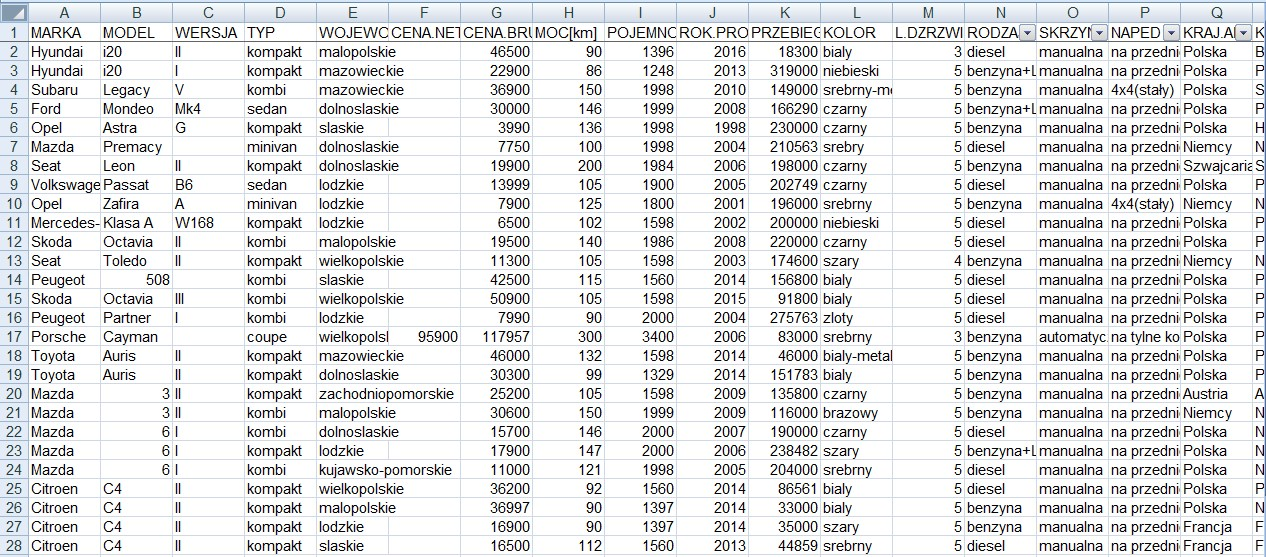
\includegraphics[width=1\textwidth]{zbior2}
%\caption{Podgląd stworzonego zbioru}
%\label{fig:obrazek1}
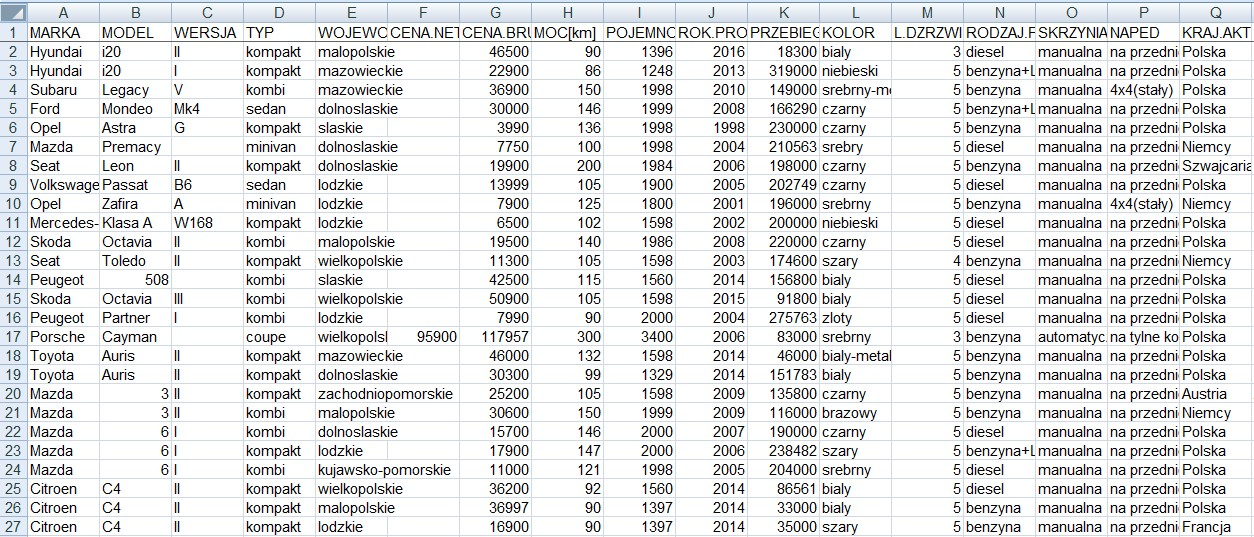
\includegraphics[width=1\textwidth]{img/zbior3.jpg}
\caption{Podgląd stworzonego zbioru}
\label{fig:obrazek1}
\end{figure}


\subsubsection{Użyte zmienne}


W stworzonym zbiorze danych znajduje się 29 atrybutów, o~pisujących 61 różnych rekordów, tj. o~biektów reprezentowanych przez wiersze, którym przypisano pewne wartości atrybutów. Wśród zebranych danych można wyróżnić zarówno zmienne jakościowe, jak i~ilościowe. 

Zmiennymi jakościowymi są atrybuty (pisownia zgodna z~plikiem danych):
\begin{multicols}{3} 
\begin{itemize}
	\item marka,
	\item model,
	\item typ,
	\item wojewodztwo,
	\item kolor,
	\item rodzaj.paliwa,
	\item skrzynia.biegow,
	\item naped,
	\item kraj.aktualnej.rejestracji,%KRAJ.AKTUALNEJ.REJESTRACJI,
	\item kraj.pochodzenia,%KRAJ.POCHODZENIA,
	\item stan,
	\item ABS,
	\item uszkodzony,
	\item pierwszy.wlasciciel,%PIERWSZY.WLASCICIEL,
	\item kto.sprzedaje,%KTO.SPRZEDAJE,
	\item serwisowany,%SERWISOWANY,
	\item komputer.pokladowy,%KOMPUTER.POKLADOWY,
	\item ESP,
	\item klimatyzacja,%KLIMATYZACJA,
	\item bezwypadkowy,%BEZWYPADKOWY,
	\item status.pojazdu.sprowadzanego%STATUS.POJAZDU.SPROWADZONEGO.
\end{itemize}
\end{multicols}

%27.06
%Wśród zmiennych jakościowych można wyróżnić zmienne porządkowe, nominalne o~raz binarne. W~stworzonym zbiorze danych zmiennymi binarnymi są atrybuty: 
%\begin{multicols}{3}
%\begin{itemize}
%	\item pierwszy.wlasciciel,%PIERWSZY.WLASCICIEL,
%	\item ABS,
%	\item serwisowany,%SERWISOWANY,
%	\item komputer.pokladowy, %KOMPUTER.POKLADOWY
%	\item ESP,
%	\item bezwypadkowy,%BEZWYPADKOWY,
%	\item uszkodzony.%USZKODZONY.
%\end{itemize}
%\end{multicols}
%
%Pozostałe atrybuty są zmiennymi nominalnymi.
%27.06

Zmiennymi ilościowymi są atrybuty:
\begin{multicols}{3}
\begin{itemize}
 \item cena.netto,%CENA.[PLN].NETTO,
 \item cena.brutto,% CENA.[PLN].BRUTTO
 \item moc,%MOC
 \item pojemnosc.skokowa,% POJEMNOSC.SKOKOWA[cm3]
 \item rok.produkcji, %ROK.PRODUKCJI
 \item przebieg,%PRZEBIEG[km]
 \item l.drzwi. %L.DRZWI
\end{itemize}
\end{multicols}

%27.06
%Wśród zmiennych ilościowych można wyróżnić zmienne skokowe o~raz dyskretne. W~stworzonym zbiorze danych, zmiennymi skokowymi są: 
%\begin{multicols}{3}
%\begin{itemize}
%	\item moc, %MOC
%	\item pojemnosc.skokowa, %POJEMNOSC.SKOKOWA[cm3]
%	\item rok.produkcji, %ROK.PRODUKCJI
%	\item przebieg, %PRZEBIEG,
%	\item l.drzwi. %L.DRZWI
%
%\end{itemize}
%\end{multicols}
%Z kolei atrybuty: cena.netto, cena.brutto są zmiennymi ciągłymi. 
%czy zmienne porządkowe nie powinny być zaliczane do zmiennych ilościowych?
%l.drzwi powinna zostać zaliczona do zmiennych porządkowych 
%27.06

\section{Użyte programy}
Zbiór danych został umieszczony w~pliku arkusza programu Excel, z~kolei implementacje zostały stworzone w~języku R, który ma zastosowanie w~statystyce i~ekonometrii. 


\section{Implementacje wybranych metod}
W sekcji tej zaprezentujemy implementacje wybranych metod porządkowania liniowego o~raz nieliniowego. W~części dotyczącej porządkowania liniowego porównamy również wyniki porządkowania par metod: metody rang i~metody sum, metody sum i~metody Hellwiga, metody rang i~metody Hellwiga. Zostanie to przeprowadzone na~całym zbiorze o~biektów. 
Zaczniemy jednak o~d przedstawienia o~gólnych funkcji o~dpowiedzialnych za stymulacje o~raz transformacje normalizacyjne. Po to by móc następnie je wykorzystać przy prezentacji wybranych metod porządkowania nieliniowego o~raz liniowego. 
\subsection{Stymulacja zmiennych}
{
\newcommand{\VerbBar}{|}
\newcommand{\VERB}{\Verb[commandchars=\\\{\}]}

\definecolor{shadecolor}{RGB}{248,248,248}
\newenvironment{Shaded}{\begin{snugshade}}{\end{snugshade}}
\newcommand{\KeywordTok}[1]{\textcolor[rgb]{0.13,0.29,0.53}{\textbf{{#1}}}}
\newcommand{\DataTypeTok}[1]{\textcolor[rgb]{0.13,0.29,0.53}{{#1}}}
\newcommand{\DecValTok}[1]{\textcolor[rgb]{0.00,0.00,0.81}{{#1}}}
\newcommand{\BaseNTok}[1]{\textcolor[rgb]{0.00,0.00,0.81}{{#1}}}
\newcommand{\FloatTok}[1]{\textcolor[rgb]{0.00,0.00,0.81}{{#1}}}
\newcommand{\ConstantTok}[1]{\textcolor[rgb]{0.00,0.00,0.00}{{#1}}}
\newcommand{\CharTok}[1]{\textcolor[rgb]{0.31,0.60,0.02}{{#1}}}
\newcommand{\SpecialCharTok}[1]{\textcolor[rgb]{0.00,0.00,0.00}{{#1}}}
\newcommand{\StringTok}[1]{\textcolor[rgb]{0.31,0.60,0.02}{{#1}}}
\newcommand{\VerbatimStringTok}[1]{\textcolor[rgb]{0.31,0.60,0.02}{{#1}}}
\newcommand{\SpecialStringTok}[1]{\textcolor[rgb]{0.31,0.60,0.02}{{#1}}}
\newcommand{\ImportTok}[1]{{#1}}
\newcommand{\CommentTok}[1]{\textcolor[rgb]{0.56,0.35,0.01}{\textit{{#1}}}}
\newcommand{\DocumentationTok}[1]{\textcolor[rgb]{0.56,0.35,0.01}{\textbf{\textit{{#1}}}}}
\newcommand{\AnnotationTok}[1]{\textcolor[rgb]{0.56,0.35,0.01}{\textbf{\textit{{#1}}}}}
\newcommand{\CommentVarTok}[1]{\textcolor[rgb]{0.56,0.35,0.01}{\textbf{\textit{{#1}}}}}
\newcommand{\OtherTok}[1]{\textcolor[rgb]{0.56,0.35,0.01}{{#1}}}
\newcommand{\FunctionTok}[1]{\textcolor[rgb]{0.00,0.00,0.00}{{#1}}}
\newcommand{\VariableTok}[1]{\textcolor[rgb]{0.00,0.00,0.00}{{#1}}}
\newcommand{\ControlFlowTok}[1]{\textcolor[rgb]{0.13,0.29,0.53}{\textbf{{#1}}}}
\newcommand{\OperatorTok}[1]{\textcolor[rgb]{0.81,0.36,0.00}{\textbf{{#1}}}}
\newcommand{\BuiltInTok}[1]{{#1}}
\newcommand{\ExtensionTok}[1]{{#1}}
\newcommand{\PreprocessorTok}[1]{\textcolor[rgb]{0.56,0.35,0.01}{\textit{{#1}}}}
\newcommand{\AttributeTok}[1]{\textcolor[rgb]{0.77,0.63,0.00}{{#1}}}
\newcommand{\RegionMarkerTok}[1]{{#1}}
\newcommand{\InformationTok}[1]{\textcolor[rgb]{0.56,0.35,0.01}{\textbf{\textit{{#1}}}}}
\newcommand{\WarningTok}[1]{\textcolor[rgb]{0.56,0.35,0.01}{\textbf{\textit{{#1}}}}}
\newcommand{\AlertTok}[1]{\textcolor[rgb]{0.94,0.16,0.16}{{#1}}}
\newcommand{\ErrorTok}[1]{\textcolor[rgb]{0.64,0.00,0.00}{\textbf{{#1}}}}
\newcommand{\NormalTok}[1]{{#1}}
\DefineVerbatimEnvironment{Highlighting}{Verbatim}{commandchars=\\\{\}}

Poniżej zostaną przedstawione metody stymulacji zmiennych o~pisane wcześniej w~sekcji \ref{wybrane_operacje_statystyczne}. o~graniczamy
się tu do przypadku, że dana zmienna jest destymulantą i~należy
ją poddać stymulacji. W~tym celu stworzyliśmy dwie funkcje:
\begin{itemize}
\item stymulacja\_przeksztalcenie\_ilorazowe(x,y),
\item stymulacja\_przeksztalcenie\_roznicowe(x,y).
\end{itemize}
W miejscu argumentu 'x'
należy wpisać nazwę zbioru na~którym dokonywane jest porządkowanie, z
kolei w~miejscu argumentu 'y' należy podać nazwę kolumny poddanej
stymulacji, z~tym że nazwa kolumny musi zostać podana w~cudzysłowie.

\begin{Shaded}
\begin{Highlighting}[]
\NormalTok{stymulacja_przeksztalcenie_ilorazowe<-function(x,y)}
\NormalTok{\{}
  \NormalTok{for (i in }\DecValTok{1}\NormalTok{:}\KeywordTok{nrow}\NormalTok{(x))}
  \NormalTok{\{}
    \NormalTok{x[i,}\KeywordTok{which}\NormalTok{(}\KeywordTok{colnames}\NormalTok{(x)==y)]=}\DecValTok{1}\NormalTok{/x[i,}\KeywordTok{which}\NormalTok{(}\KeywordTok{colnames}\NormalTok{(x)==y)]}
  \NormalTok{\}}
  \KeywordTok{return}\NormalTok{(x)}
\NormalTok{\}}
\end{Highlighting}
\end{Shaded}

\begin{Shaded}
\begin{Highlighting}[]
\NormalTok{stymulacja_przeksztalcenie_roznicowe<-function(x,y)}
\NormalTok{\{}
  \NormalTok{max_wartosc=}\KeywordTok{max}\NormalTok{(x[}\KeywordTok{which}\NormalTok{(}\KeywordTok{colnames}\NormalTok{(x)==y)])}
  \NormalTok{for (i in }\DecValTok{1}\NormalTok{:}\KeywordTok{nrow}\NormalTok{(x))}
  \NormalTok{\{}
    \NormalTok{x[i,}\KeywordTok{which}\NormalTok{(}\KeywordTok{colnames}\NormalTok{(x)==y)]=max_wartosc-x[i,}\KeywordTok{which}\NormalTok{(}\KeywordTok{colnames}\NormalTok{(x)==y)]}
  \NormalTok{\}}
  \KeywordTok{return}\NormalTok{(x)}
\NormalTok{\}}
\end{Highlighting}
\end{Shaded}

\begin{uwaga} Stymulacja zmiennych dokonywana jest pojedynczo, tj. jeżeli w
naszym zbiorze jest wiele zmiennych mających charakter destymulanty, dla
każdej z~nich musimy użyć funkcji, na~sam koniec nadpisać nasz zbiór,
tym nowym wystymulowanym, dzięki czemu przekształcenia zostaną zapisane.
\end{uwaga}

}
\subsection{Transformacje normalizacyjne}
Poniżej zostaną przedstawione o~gólne funkcje transformacji normalizacyjnej - standaryzacja, unitaryzacja, przekształcenie ilorazowe. Podobnie jak metody stymulacji zmiennych, zostały o~ne wcześniej o~mówione w~sekcji \ref{wybrane_operacje_statystyczne}. Aby wywołać którąś z~poniższych funkcji, należy w~miejsce 'x' wpisać nazwę zbioru.

{
\newcommand{\VerbBar}{|}
\newcommand{\VERB}{\Verb[commandchars=\\\{\}]}

\definecolor{shadecolor}{RGB}{248,248,248}
\newenvironment{Shaded}{\begin{snugshade}}{\end{snugshade}}
\newcommand{\KeywordTok}[1]{\textcolor[rgb]{0.13,0.29,0.53}{\textbf{{#1}}}}
\newcommand{\DataTypeTok}[1]{\textcolor[rgb]{0.13,0.29,0.53}{{#1}}}
\newcommand{\DecValTok}[1]{\textcolor[rgb]{0.00,0.00,0.81}{{#1}}}
\newcommand{\BaseNTok}[1]{\textcolor[rgb]{0.00,0.00,0.81}{{#1}}}
\newcommand{\FloatTok}[1]{\textcolor[rgb]{0.00,0.00,0.81}{{#1}}}
\newcommand{\ConstantTok}[1]{\textcolor[rgb]{0.00,0.00,0.00}{{#1}}}
\newcommand{\CharTok}[1]{\textcolor[rgb]{0.31,0.60,0.02}{{#1}}}
\newcommand{\SpecialCharTok}[1]{\textcolor[rgb]{0.00,0.00,0.00}{{#1}}}
\newcommand{\StringTok}[1]{\textcolor[rgb]{0.31,0.60,0.02}{{#1}}}
\newcommand{\VerbatimStringTok}[1]{\textcolor[rgb]{0.31,0.60,0.02}{{#1}}}
\newcommand{\SpecialStringTok}[1]{\textcolor[rgb]{0.31,0.60,0.02}{{#1}}}
\newcommand{\ImportTok}[1]{{#1}}
\newcommand{\CommentTok}[1]{\textcolor[rgb]{0.56,0.35,0.01}{\textit{{#1}}}}
\newcommand{\DocumentationTok}[1]{\textcolor[rgb]{0.56,0.35,0.01}{\textbf{\textit{{#1}}}}}
\newcommand{\AnnotationTok}[1]{\textcolor[rgb]{0.56,0.35,0.01}{\textbf{\textit{{#1}}}}}
\newcommand{\CommentVarTok}[1]{\textcolor[rgb]{0.56,0.35,0.01}{\textbf{\textit{{#1}}}}}
\newcommand{\OtherTok}[1]{\textcolor[rgb]{0.56,0.35,0.01}{{#1}}}
\newcommand{\FunctionTok}[1]{\textcolor[rgb]{0.00,0.00,0.00}{{#1}}}
\newcommand{\VariableTok}[1]{\textcolor[rgb]{0.00,0.00,0.00}{{#1}}}
\newcommand{\ControlFlowTok}[1]{\textcolor[rgb]{0.13,0.29,0.53}{\textbf{{#1}}}}
\newcommand{\OperatorTok}[1]{\textcolor[rgb]{0.81,0.36,0.00}{\textbf{{#1}}}}
\newcommand{\BuiltInTok}[1]{{#1}}
\newcommand{\ExtensionTok}[1]{{#1}}
\newcommand{\PreprocessorTok}[1]{\textcolor[rgb]{0.56,0.35,0.01}{\textit{{#1}}}}
\newcommand{\AttributeTok}[1]{\textcolor[rgb]{0.77,0.63,0.00}{{#1}}}
\newcommand{\RegionMarkerTok}[1]{{#1}}
\newcommand{\InformationTok}[1]{\textcolor[rgb]{0.56,0.35,0.01}{\textbf{\textit{{#1}}}}}
\newcommand{\WarningTok}[1]{\textcolor[rgb]{0.56,0.35,0.01}{\textbf{\textit{{#1}}}}}
\newcommand{\AlertTok}[1]{\textcolor[rgb]{0.94,0.16,0.16}{{#1}}}
\newcommand{\ErrorTok}[1]{\textcolor[rgb]{0.64,0.00,0.00}{\textbf{{#1}}}}
\newcommand{\NormalTok}[1]{{#1}}
\DefineVerbatimEnvironment{Highlighting}{Verbatim}{commandchars=\\\{\}}



\begin{Shaded}
\begin{Highlighting}[]
\NormalTok{standaryzacja<-function(x)}
\NormalTok{\{}
  \NormalTok{suma=}\DecValTok{0}
  \NormalTok{srednia=}\DecValTok{0}
  \NormalTok{odchylenie=}\DecValTok{0}
  \NormalTok{for (j in }\DecValTok{2}\NormalTok{:}\KeywordTok{ncol}\NormalTok{(x))}
  \NormalTok{\{}
    \NormalTok{suma[j]=}\KeywordTok{sum}\NormalTok{(x[j])}
    \NormalTok{srednia[j]=suma[j]/}\KeywordTok{nrow}\NormalTok{(x)}
    \NormalTok{suma_kwadratow=}\DecValTok{0}
    \NormalTok{kwadrat=}\DecValTok{0}
    \NormalTok{for(i in }\DecValTok{1}\NormalTok{:}\KeywordTok{nrow}\NormalTok{(x))}
    \NormalTok{\{}
      \NormalTok{kwadrat=(x[i,j]-srednia[j])^}\DecValTok{2}
      \NormalTok{suma_kwadratow=suma_kwadratow+kwadrat}
    \NormalTok{\}}
    \NormalTok{odchylenie[j]=}\KeywordTok{sqrt}\NormalTok{(suma_kwadratow/}\KeywordTok{nrow}\NormalTok{(x))  }
    \NormalTok{for (i in }\DecValTok{1}\NormalTok{:}\KeywordTok{nrow}\NormalTok{(x))}
    \NormalTok{\{}
      \NormalTok{x[i,j]=(x[i,j]-srednia[j])/odchylenie[j]}
    \NormalTok{\} }
  \NormalTok{\}}
  \KeywordTok{return}\NormalTok{(x)}
\NormalTok{\}}
\end{Highlighting}
\end{Shaded}


\begin{Shaded}
\begin{Highlighting}[]
\NormalTok{unitaryzacja<-function(x)}
\NormalTok{\{}
  \NormalTok{maksi=}\DecValTok{0}
  \NormalTok{minim=}\DecValTok{0}
  \NormalTok{for (j in }\DecValTok{2}\NormalTok{:}\KeywordTok{ncol}\NormalTok{(x))}
  \NormalTok{\{}
    \NormalTok{maksi[j]=}\KeywordTok{max}\NormalTok{(x[j])}
    \NormalTok{minim[j]=}\KeywordTok{min}\NormalTok{(x[j])}
    \NormalTok{for (i in }\DecValTok{1}\NormalTok{:}\KeywordTok{nrow}\NormalTok{(x))}
    \NormalTok{\{}
    \NormalTok{x[i,j]=(x[i,j]-minim[j])/(maksi[j]-minim[j])}
    \NormalTok{\}}
  \NormalTok{\}}
\KeywordTok{return}\NormalTok{(x)}
\NormalTok{\}}
\end{Highlighting}
\end{Shaded}


\begin{Shaded}
\begin{Highlighting}[]
\NormalTok{przeksztalcenie_ilorazowe<-function(x)}
\NormalTok{\{}
  \NormalTok{suma=}\DecValTok{0}
  \NormalTok{srednia=}\DecValTok{0}
  \NormalTok{for (j in }\DecValTok{2}\NormalTok{:}\KeywordTok{ncol}\NormalTok{(x))}
  \NormalTok{\{}
    \NormalTok{suma[j]=}\KeywordTok{sum}\NormalTok{(x[j])}
    \NormalTok{srednia[j]=suma[j]/}\KeywordTok{nrow}\NormalTok{(x)}
    \NormalTok{for(i in }\DecValTok{1}\NormalTok{:}\KeywordTok{nrow}\NormalTok{(x))}
    \NormalTok{\{}
      \NormalTok{x[i,j]=x[i,j]/srednia[j]}
    \NormalTok{\}}
  \NormalTok{\} }
\KeywordTok{return}\NormalTok{(x)}
\NormalTok{\}}
\end{Highlighting}
\end{Shaded}

}



\subsection{Metody porządkowania nieliniowego}
{
%% dane z~eksperymentu "metoda nieliniowa duzy.Rmd"


\newcommand{\VerbBar}{|}
\newcommand{\VERB}{\Verb[commandchars=\\\{\}]}

\definecolor{shadecolor}{RGB}{248,248,248}
\newenvironment{Shaded}{\begin{snugshade}}{\end{snugshade}}
\newcommand{\KeywordTok}[1]{\textcolor[rgb]{0.13,0.29,0.53}{\textbf{{#1}}}}
\newcommand{\DataTypeTok}[1]{\textcolor[rgb]{0.13,0.29,0.53}{{#1}}}
\newcommand{\DecValTok}[1]{\textcolor[rgb]{0.00,0.00,0.81}{{#1}}}
\newcommand{\BaseNTok}[1]{\textcolor[rgb]{0.00,0.00,0.81}{{#1}}}
\newcommand{\FloatTok}[1]{\textcolor[rgb]{0.00,0.00,0.81}{{#1}}}
\newcommand{\ConstantTok}[1]{\textcolor[rgb]{0.00,0.00,0.00}{{#1}}}
\newcommand{\CharTok}[1]{\textcolor[rgb]{0.31,0.60,0.02}{{#1}}}
\newcommand{\SpecialCharTok}[1]{\textcolor[rgb]{0.00,0.00,0.00}{{#1}}}
\newcommand{\StringTok}[1]{\textcolor[rgb]{0.31,0.60,0.02}{{#1}}}
\newcommand{\VerbatimStringTok}[1]{\textcolor[rgb]{0.31,0.60,0.02}{{#1}}}
\newcommand{\SpecialStringTok}[1]{\textcolor[rgb]{0.31,0.60,0.02}{{#1}}}
\newcommand{\ImportTok}[1]{{#1}}
\newcommand{\CommentTok}[1]{\textcolor[rgb]{0.56,0.35,0.01}{\textit{{#1}}}}
\newcommand{\DocumentationTok}[1]{\textcolor[rgb]{0.56,0.35,0.01}{\textbf{\textit{{#1}}}}}
\newcommand{\AnnotationTok}[1]{\textcolor[rgb]{0.56,0.35,0.01}{\textbf{\textit{{#1}}}}}
\newcommand{\CommentVarTok}[1]{\textcolor[rgb]{0.56,0.35,0.01}{\textbf{\textit{{#1}}}}}
\newcommand{\OtherTok}[1]{\textcolor[rgb]{0.56,0.35,0.01}{{#1}}}
\newcommand{\FunctionTok}[1]{\textcolor[rgb]{0.00,0.00,0.00}{{#1}}}
\newcommand{\VariableTok}[1]{\textcolor[rgb]{0.00,0.00,0.00}{{#1}}}
\newcommand{\ControlFlowTok}[1]{\textcolor[rgb]{0.13,0.29,0.53}{\textbf{{#1}}}}
\newcommand{\OperatorTok}[1]{\textcolor[rgb]{0.81,0.36,0.00}{\textbf{{#1}}}}
\newcommand{\BuiltInTok}[1]{{#1}}
\newcommand{\ExtensionTok}[1]{{#1}}
\newcommand{\PreprocessorTok}[1]{\textcolor[rgb]{0.56,0.35,0.01}{\textit{{#1}}}}
\newcommand{\AttributeTok}[1]{\textcolor[rgb]{0.77,0.63,0.00}{{#1}}}
\newcommand{\RegionMarkerTok}[1]{{#1}}
\newcommand{\InformationTok}[1]{\textcolor[rgb]{0.56,0.35,0.01}{\textbf{\textit{{#1}}}}}
\newcommand{\WarningTok}[1]{\textcolor[rgb]{0.56,0.35,0.01}{\textbf{\textit{{#1}}}}}
\newcommand{\AlertTok}[1]{\textcolor[rgb]{0.94,0.16,0.16}{{#1}}}
\newcommand{\ErrorTok}[1]{\textcolor[rgb]{0.64,0.00,0.00}{\textbf{{#1}}}}
\newcommand{\NormalTok}[1]{{#1}}
\DefineVerbatimEnvironment{Highlighting}{Verbatim}{commandchars=\\\{\}}

%TODO

%\subsubsection{Wstęp}\label{wstep}

Zostanie tutaj zaprezentowane zastosowanie nieliniowego porządkowania
danych przy pomocy istniejących funkcji biblioteki cluster, w~której to
funkcja agnes umożliwia uporządkowanie zbioru po wyborze
odpowiedniej metody aglomeracyjnej. Mamy tu do wyboru metody: single -
metoda najbliższego sąsiedztwa, complete - metoda najdalszego
sąsiedztwa, ward - metoda Warda, average - metoda średniej między
grupowej. Poniżej zostanie zaprezentowane zastosowanie metod single o~raz
complete wraz z~porównaniem wyników porządkowania.

\subsubsection{Import danych}\label{import-danych}

Na początku należy jednak zaimportować dane, które chcemy poddać porządkowaniu.
W tym celu należy zaimportować biblotekę readxl - gdyż dane pobieramy z
excela, a w~kolejnym kroku wywołujemy plik, podając jego ścieżkę 
z rozszerzeniem xlsx. My użyjemy tutaj zbioru wszystkich o~biektów,
będących o~fertami sprzedaży aut.

\begin{Shaded}
\begin{Highlighting}[]
\KeywordTok{library}\NormalTok{(readxl)}
\NormalTok{zbior_danych <-}\StringTok{ }\KeywordTok{read_excel}\NormalTok{(}\StringTok{"datasets/zbior_danych.xlsx"}\NormalTok{, }
                           \DataTypeTok{sheet =} \StringTok{"DANE_INNA_WERSJA"}\NormalTok{)}
\end{Highlighting}
\end{Shaded}

Podgląd danych:

\begin{Shaded}
\begin{Highlighting}[]
\KeywordTok{head}\NormalTok{(zbior_danych)}
\end{Highlighting}
\end{Shaded}

\begin{verbatim}
## # A tibble: 6 x 30
##      Nr MARKA   MODEL   WERSJA TYP     WOJEWODZTWO  `CENA.NETTO_[pln]`
##   <dbl> <chr>   <chr>   <chr>  <chr>   <chr>                     <dbl>
## 1  1.00 Hyundai i20     II     kompakt malopolskie                  NA
## 2  2.00 Hyundai i20     I      kompakt mazowieckie                  NA
## 3  3.00 Subaru  Legacy  V      kombi   mazowieckie                  NA
## 4  4.00 Ford    Mondeo  Mk4    sedan   dolnoslaskie                 NA
## 5  5.00 o~pel    Astra   G      kompakt slaskie                      NA
## 6  6.00 Mazda   Premacy <NA>   minivan dolnoslaskie                 NA
## # ... with 23 more variables: `CENA.BRUTTO_[pln]` <dbl>, `MOC_[km]` <dbl>,
## #   `POJEMNOSC.SKOKOWA_[cm3]` <dbl>, ROK.PRODUKCJI <dbl>, `PRZEBIEG_[km]`
## #   <dbl>, KOLOR <chr>, L.DZRZWI <dbl>, RODZAJ.PALIWA <chr>,
## #   SKRZYNIA.BIEGOW <chr>, NAPED <chr>, KRAJ.AKTUALNEJ.REJESTRACJI <chr>,
## #   KRAJ.POCHODZENIA <chr>, STATUS.POJAZDU.SPROWADZONEGO <chr>,
## #   PIERWSZY.WLASCICIEL <dbl>, KTO.SPRZEDAJE <chr>, STAN <chr>,
## #   SERWISOWANY <dbl>, ABS <dbl>, KOMPUTER.POKLADOWY <dbl>, ESP <dbl>,
## #   KLIMATYZAJCA <dbl>, BEZWYPADKOWY <dbl>, USZKODZONY <dbl>
\end{verbatim}

\subsubsection{Podzbiór danych}\label{podzbior-danych}

W kolejnym, kroku po przyjrzeniu się zbiorowi danych, użytkownik musi
zadecydować na~których danych ilościowych chce pracować - ważna jest
znajomość danych. Dodatkowo pierwszą kolumną musi być kolumna
zawierająca numery indeksów o~biektów, ze względu na~to, że jako wynik
zastosowania funkcji o~dpowiedzialnej za porządkowanie, zostaną zwrócone
w kolejności malejącej numery indeksów, mówiące o~ kolejności
uporządkowania. W~związku z~tym, za pomocą poniższej procedury
użytkownik tworzy podzbiór zaimportowanego zbioru, gdzie w~cudzysłowie
wpisuje nazwy kolumn zawierających zmienne ilościowe, wybrane do
porządkowania (zakładamy, że podzbiór będzie nazywał się
dane\_porzadkowanie)). Wybranymi kolumnami są: cena, moc, pojemność, rok produkcji,
przebieg.

\begin{Shaded}
\begin{Highlighting}[]
\NormalTok{dane_porzadkowanie<-zbior_danych[}\KeywordTok{c}\NormalTok{(}\StringTok{"Nr"}\NormalTok{,}\StringTok{"CENA.BRUTTO_[pln]"}\NormalTok{,}\StringTok{"MOC_[km]"}\NormalTok{,}
                                   \StringTok{"POJEMNOSC.SKOKOWA_[cm3]"}\NormalTok{,}
                                  \StringTok{"ROK.PRODUKCJI"}\NormalTok{,}\StringTok{"PRZEBIEG_[km]"}\NormalTok{)]}
\end{Highlighting}
\end{Shaded}

\subsubsection{Transformacje danych}\label{transformacje-danych}

Przed samym porządkowaniem, wymagane jest aby zmienne miały charakter
stymulant o~raz by zostały poddane transformacji normalizacyjnej. Aby
funkcja dokonująca porządkowania dawała poprawny wynik, użytkownik musi
zająć się transformacją przed jej zastosowaniem. Poniżej podaliśmy tego
przykład. Dla zmiennych, które stymulantami nie są, należy dokonać
stymulacji. Wśród zmiennych poddanych porządkowaniu, do stymulant
nie należy zmienna zmienna: przebieg - jest destymulantą, w~związku z
tym, została przekształcona na~stymulantę, za pomocą przekształcenia
ilorazowego.


\begin{Shaded}
\begin{Highlighting}[]
\NormalTok{dane_porzadkowanie<-}\KeywordTok{stymulacja_przeksztalcenie_ilorazowe}\NormalTok{(dane_porzadkowanie,}
\StringTok{"PRZEBIEG_[km]"}\NormalTok{)}
\end{Highlighting}
\end{Shaded}

W celu uzyskania porównywalności między zmiennymi, zostały o~ne poddane
transformacji normalizacyjnej - unitaryzacji.

\begin{Shaded}
\begin{Highlighting}[]
\NormalTok{dane_porzadkowanie<-}\KeywordTok{unitaryzacja}\NormalTok{(dane_porzadkowanie)}
\end{Highlighting}
\end{Shaded}

\subsubsection{Zastosowanie metod aglomeracyjnych}


Chcąc zastosować funkcję agnes, należy w~pierwszej kolejności wyznaczyć
macierz o~dległości pomiędzy wszystkimi parami o~biektów. Do wyznaczenia
odległości zostanie użyta metryka euklidesowa - w~tym celu zostanie
wykorzystania funkcja dist(x, method=``'') - w~miejsce 'x' należy wpisać
nazwę tabeli zawierających dane do uporządkowania, a w~nawiasie{[},{]}
na miejscu drugiej współrzędnej należy podać wektor kolumn, na~podstawie
którego wartości zostanie wyznaczona macierz o~dległości. W~miejsce
argumentu method należy wpisać nazwę metryki na~podstawie której zostanie
obliczona o~dległość - w~naszym przypadku będzie to euclidean -
euklidesowa.

\begin{Shaded}
\begin{Highlighting}[]
\NormalTok{odleglosci <-}\StringTok{ }\KeywordTok{dist}\NormalTok{(dane_porzadkowanie[,}\KeywordTok{c}\NormalTok{(}\StringTok{"CENA.BRUTTO_[pln]"}\NormalTok{,}\StringTok{"MOC_[km]"}\NormalTok{,}
            \StringTok{"POJEMNOSC.SKOKOWA_[cm3]"}\NormalTok{,}\StringTok{"ROK.PRODUKCJI"}\NormalTok{,}\StringTok{"PRZEBIEG_[km]"}\NormalTok{)],                                           }\DataTypeTok{method =} \StringTok{"euclidean"}\NormalTok{)}
\end{Highlighting}
\end{Shaded}

Następnie należy zaimportować bibliotekę cluster, by móc skorzystać z
metod aglomeracyjnych. Jak już zostało wspomnanie we wstępnie, wywołanie
metod aglomeracyjnych o~dbywa się dzięki funkcji agnes(x, method=``'') .
W miejsce argumentu 'x' - zostanie podana wyznaczona macierz o~dległości z
kolei, w~kolejnym argumencie - method zostanie podana reguła wyznaczania
odległości pomiędzy nową grupą a pozostałymi o~biektów. Regułą tą może
być metoda najbliższego sąsiedztwa, najdalszego, Warda lub średniej
między grupowej. My wykorzystamy metodę najbliższego sąsiedztwa o~raz
najdalszego.

\begin{Shaded}
\begin{Highlighting}[]
\KeywordTok{library}\NormalTok{(cluster)}
\NormalTok{metoda_najblizszego <-}\StringTok{ }\KeywordTok{agnes}\NormalTok{(odleglosci, }\DataTypeTok{method =} \StringTok{"single"}\NormalTok{)}
\NormalTok{metoda_najdalszego<-}\StringTok{ }\KeywordTok{agnes}\NormalTok{(odleglosci, }\DataTypeTok{method =} \StringTok{"complete"}\NormalTok{)}
\end{Highlighting}
\end{Shaded}

Ostatni etap to graficzne zaprezentowanie wyniku w~postaci dendrogramu.
W tym celu należy zaimportować bibliotekę factoextra, w~której to jest
funkcja fviz\_dend(x, main = ``''). W~miejsce argumentu x należy wpisać
nazwę o~biektu powstałego przy pomocy funkcji agnes, main to tytuł
wykresu. Dodatkowo na~osi pionowej zaprezentowane są o~dległości między
obiektami, z~kolei na~osi poziomej znajdują się numery indeksów
obiektów.

Dendrogram dla metody najbliższego sąsiada, prezentuje się następująco:

\begin{Shaded}
\begin{Highlighting}[]
\KeywordTok{library}\NormalTok{(factoextra)}
\KeywordTok{fviz_dend}\NormalTok{(metoda_najblizszego, }\DataTypeTok{lwd=}\FloatTok{0.1}\NormalTok{, }\DataTypeTok{cex=}\FloatTok{0.45}\NormalTok{, }
\DataTypeTok{main =} \StringTok{"Metoda najbliższego sąsiedztwa"}\NormalTok{)}
\end{Highlighting}
\end{Shaded}

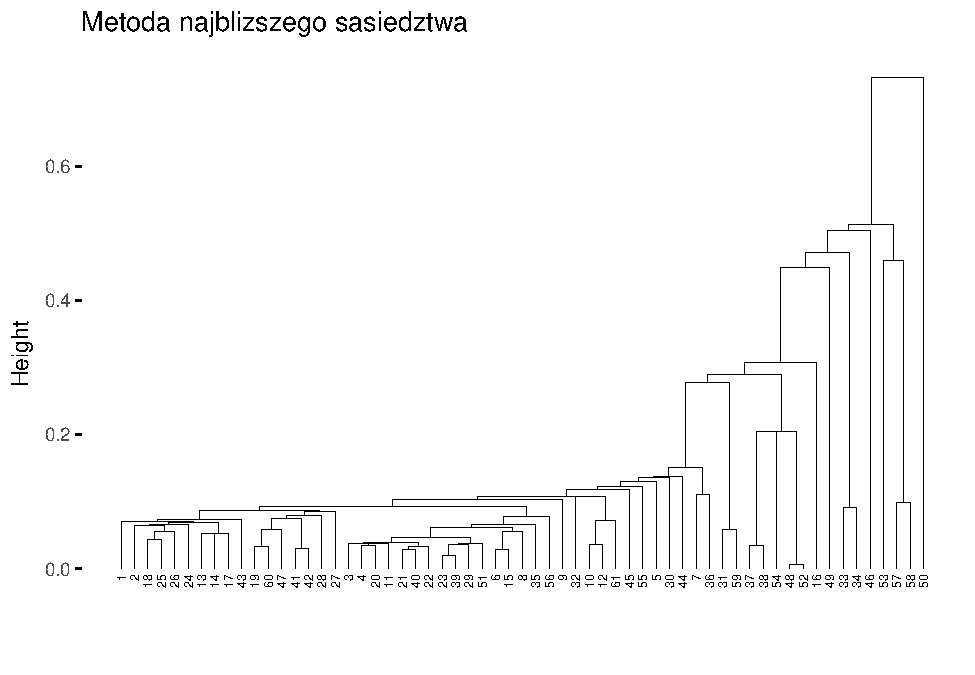
\includegraphics{Metoda_nieliniowa_duzy_files/figure-latex/unnamed-chunk-9-1.pdf}

Dendrogram dla metody najdalszego sąsiada, wygląda natomiast:

\begin{Shaded}
\begin{Highlighting}[]
\KeywordTok{fviz_dend}\NormalTok{(metoda_najdalszego, }\DataTypeTok{lwd=}\FloatTok{0.1}\NormalTok{, }\DataTypeTok{cex=}\FloatTok{0.45}\NormalTok{, }
\DataTypeTok{main =} \StringTok{"Metoda najdalszego sąsiedztwa"}\NormalTok{)}
\end{Highlighting}
\end{Shaded}

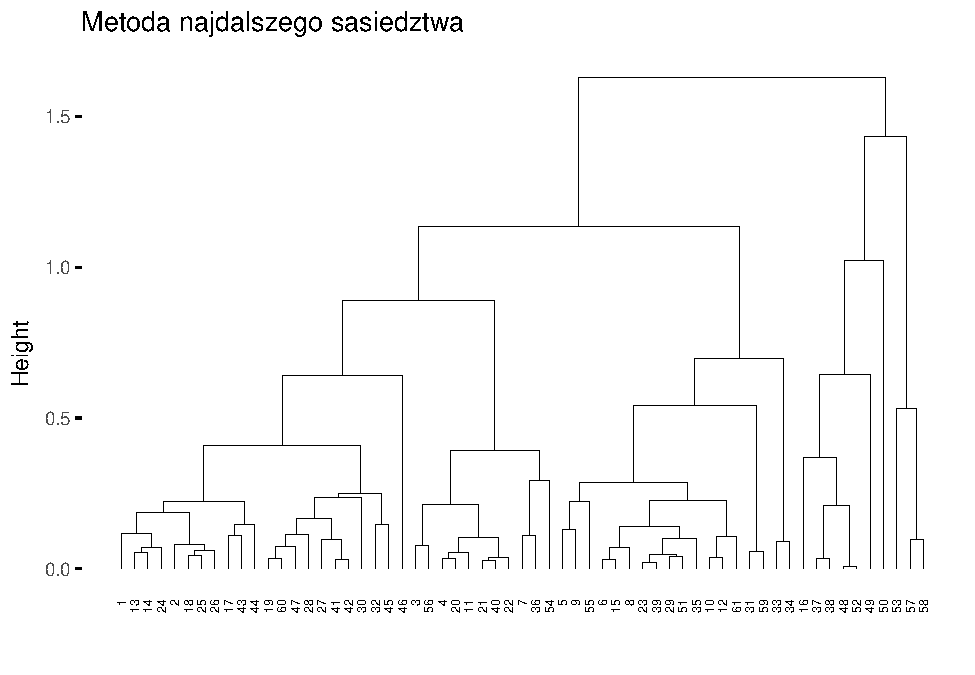
\includegraphics{Metoda_nieliniowa_duzy_files/figure-latex/unnamed-chunk-10-1.pdf}

\subsubsection{Porównanie wyników uporządkowania}

W przypadku dendrogramu uzyskanego metodą najdalszego sąsiedztwa można
zauważyć większą o~dległość wiązań niż dla metody najbliższego
sąsiedztwa, które to o~brazują o~dległość między grupami. Dodatkowo
obiekty charakteryzujące się najbardziej korzystnym wartości zmiennych,
zostały pogrupowane w~jedną grupę (tu mowa o~ o~biektach o~ numerach
indeksów 49, 50, 53, 57, 58), natomiast w~przypadku metody najbliższego
sąsiedztwa o~biekty te zostały rozdzielone na~pojedyncze grupy. Można
również zauważyć, że w~przypadku uporządkowania metodą najdalszego
sąsiedztwa o~biekty tworzą pewnego rodzaju podgrupy - skupiska, z~kolei w
przypadku uporządkowania metodą najbliższego sąsiada, wynik
porządkowania można porównać do wyglądu lawiny, lub góry, u której
podnóża znajdują się o~biekty o~ najniższych wartościach o~pisywanych je
zmiennych, które to następnie łączą się i~dochodzą do szczytu, który stanowią
obiekty o~ najwyższych wartościach o~pisywanych je zmiennych.

}
\subsection{Metody porządkowania liniowego}\label{porzadkowanie-liniowe}
{

\newcommand{\VerbBar}{|}
\newcommand{\VERB}{\Verb[commandchars=\\\{\}]}

\definecolor{shadecolor}{RGB}{248,248,248}
\newenvironment{Shaded}{\begin{snugshade}}{\end{snugshade}}
\newcommand{\KeywordTok}[1]{\textcolor[rgb]{0.13,0.29,0.53}{\textbf{{#1}}}}
\newcommand{\DataTypeTok}[1]{\textcolor[rgb]{0.13,0.29,0.53}{{#1}}}
\newcommand{\DecValTok}[1]{\textcolor[rgb]{0.00,0.00,0.81}{{#1}}}
\newcommand{\BaseNTok}[1]{\textcolor[rgb]{0.00,0.00,0.81}{{#1}}}
\newcommand{\FloatTok}[1]{\textcolor[rgb]{0.00,0.00,0.81}{{#1}}}
\newcommand{\ConstantTok}[1]{\textcolor[rgb]{0.00,0.00,0.00}{{#1}}}
\newcommand{\CharTok}[1]{\textcolor[rgb]{0.31,0.60,0.02}{{#1}}}
\newcommand{\SpecialCharTok}[1]{\textcolor[rgb]{0.00,0.00,0.00}{{#1}}}
\newcommand{\StringTok}[1]{\textcolor[rgb]{0.31,0.60,0.02}{{#1}}}
\newcommand{\VerbatimStringTok}[1]{\textcolor[rgb]{0.31,0.60,0.02}{{#1}}}
\newcommand{\SpecialStringTok}[1]{\textcolor[rgb]{0.31,0.60,0.02}{{#1}}}
\newcommand{\ImportTok}[1]{{#1}}
\newcommand{\CommentTok}[1]{\textcolor[rgb]{0.56,0.35,0.01}{\textit{{#1}}}}
\newcommand{\DocumentationTok}[1]{\textcolor[rgb]{0.56,0.35,0.01}{\textbf{\textit{{#1}}}}}
\newcommand{\AnnotationTok}[1]{\textcolor[rgb]{0.56,0.35,0.01}{\textbf{\textit{{#1}}}}}
\newcommand{\CommentVarTok}[1]{\textcolor[rgb]{0.56,0.35,0.01}{\textbf{\textit{{#1}}}}}
\newcommand{\OtherTok}[1]{\textcolor[rgb]{0.56,0.35,0.01}{{#1}}}
\newcommand{\FunctionTok}[1]{\textcolor[rgb]{0.00,0.00,0.00}{{#1}}}
\newcommand{\VariableTok}[1]{\textcolor[rgb]{0.00,0.00,0.00}{{#1}}}
\newcommand{\ControlFlowTok}[1]{\textcolor[rgb]{0.13,0.29,0.53}{\textbf{{#1}}}}
\newcommand{\OperatorTok}[1]{\textcolor[rgb]{0.81,0.36,0.00}{\textbf{{#1}}}}
\newcommand{\BuiltInTok}[1]{{#1}}
\newcommand{\ExtensionTok}[1]{{#1}}
\newcommand{\PreprocessorTok}[1]{\textcolor[rgb]{0.56,0.35,0.01}{\textit{{#1}}}}
\newcommand{\AttributeTok}[1]{\textcolor[rgb]{0.77,0.63,0.00}{{#1}}}
\newcommand{\RegionMarkerTok}[1]{{#1}}
\newcommand{\InformationTok}[1]{\textcolor[rgb]{0.56,0.35,0.01}{\textbf{\textit{{#1}}}}}
\newcommand{\WarningTok}[1]{\textcolor[rgb]{0.56,0.35,0.01}{\textbf{\textit{{#1}}}}}
\newcommand{\AlertTok}[1]{\textcolor[rgb]{0.94,0.16,0.16}{{#1}}}
\newcommand{\ErrorTok}[1]{\textcolor[rgb]{0.64,0.00,0.00}{\textbf{{#1}}}}
\newcommand{\NormalTok}[1]{{#1}}
\DefineVerbatimEnvironment{Highlighting}{Verbatim}{commandchars=\\\{\}}


Zostaną tu zaprezentowane metody liniowe: metoda sum, rang o~raz Hellwiga. Dla wszystkich metod będziemy korzystać z~tego samego zbioru danych, który jest podzbiorem wyjściowego zbioru - zawiera 8 najbardziej różniących się o~biektów. Różnice dla każdej z~metod będą zaczynały się o~d sekcji związanej z~transformacją danych. 

\subsubsection{Import danych}\label{import-danych}
Wobec powyższego, podobnie jak przy metodach porządkowania nieliniowego, użytkownik musi zaimportować dane, które chce poddać porządkowaniu. 


\begin{Shaded}
\begin{Highlighting}[]
\KeywordTok{library}\NormalTok{(readxl)}
\NormalTok{zbior_danych <-}\StringTok{ }\KeywordTok{read_excel}\NormalTok{(}\StringTok{"datasets/8_Rozniacych_sie_obiektow.xlsx"}\NormalTok{, }
                           \DataTypeTok{sheet =} \StringTok{"Arkusz1"}\NormalTok{, }\DataTypeTok{col_types =} \KeywordTok{c}\NormalTok{(}\StringTok{"numeric"}\NormalTok{,}\StringTok{"text"}\NormalTok{, }
                           \StringTok{"text"}\NormalTok{, }\StringTok{"text"}\NormalTok{, }\StringTok{"text"}\NormalTok{, }\StringTok{"text"}\NormalTok{,                                                                              }\StringTok{"blank"}\NormalTok{,}\StringTok{"numeric"}\NormalTok{, }\StringTok{"numeric"}\NormalTok{, }\StringTok{"numeric"}\NormalTok{, }
                              \StringTok{"numeric"}\NormalTok{, }\StringTok{"numeric"}\NormalTok{, }\StringTok{"text"}\NormalTok{,  }\StringTok{"numeric"}\NormalTok{, }
                              \StringTok{"text"}\NormalTok{, }\StringTok{"text"}\NormalTok{, }\StringTok{"text"}\NormalTok{, }\StringTok{"text"}\NormalTok{,}\StringTok{"text"}\NormalTok{, }
                                  \StringTok{"text"}\NormalTok{, }\StringTok{"numeric"}\NormalTok{, }\StringTok{"text"}\NormalTok{, }\StringTok{"text"}\NormalTok{, }
                                   \StringTok{"text"}\NormalTok{, }\StringTok{"numeric"}\NormalTok{, }\StringTok{"numeric"}\NormalTok{,                                                                              }\StringTok{"numeric"}\NormalTok{, }
                                   \StringTok{"numeric"}\NormalTok{, }\StringTok{"numeric"}\NormalTok{, }\StringTok{"numeric"}\NormalTok{))}
\end{Highlighting}
\end{Shaded}



Podgląd danych:

\begin{Shaded}
\begin{Highlighting}[]
\KeywordTok{head}\NormalTok{(zbior_danych)}
\end{Highlighting}
\end{Shaded}

\begin{verbatim}
## # A tibble: 6 x 29
##      Nr MARKA  MODEL  WERSJA TYP   WOJEWODZTWO `CENA.BRUTTO_[p~ `MOC_[km]`
##   <dbl> <chr>  <chr>  <chr>  <chr> <chr>                  <dbl>      <dbl>
## 1  1.00 Mazda  3      II     komp~ zachodniop~            25200        105
## 2  2.00 Jaguar XF     X260   kombi dolnoslask~           323600        240
## 3  3.00 Subaru B9 Tr~ <NA>   suv   malopolskie            38900        245
## 4  4.00 Volks~ Golf   VII    kombi lodzkie               113900        150
## 5  5.00 Peuge~ 508    <NA>   kombi slaskie                42500        115
## 6  6.00 o~pel   Antara <NA>   suv   lodzkie                24000        150
## # ... with 21 more variables: `POJEMNOSC.SKOKOWA_[cm3]` <dbl>,
## #   ROK.PRODUKCJI <dbl>, `PRZEBIEG_[km]` <dbl>, KOLOR <chr>, L.DZRZWI
## #   <dbl>, RODZAJ.PALIWA <chr>, SKRZYNIA.BIEGOW <chr>, NAPED <chr>,
## #   KRAJ.AKTUALNEJ.REJESTRACJI <chr>, KRAJ.POCHODZENIA <chr>,
## #   STATUS.POJAZDU.SPROWADZONEGO <chr>, PIERWSZY.WLASCICIEL <dbl>,
## #   KTO.SPRZEDAJE <chr>, STAN <chr>, SERWISOWANY <chr>, ABS <dbl>,
## #   KOMPUTER.POKLADOWY <dbl>, ESP <dbl>, KLIMATYZAJCA <dbl>, BEZWYPADKOWY
## #   <dbl>, USZKODZONY <dbl>
\end{verbatim}

\subsubsection{Podzbiór danych}\label{podzbior-danych}

W kolejnym, kroku po przyjrzeniu się zbiorowi danych, użytkownik musi
zadecydować na~których danych ilościowych chce pracować - ważna jest
znajomość danych. Dodatkowo pierwszą kolumną musi być kolumna
zawierająca numery indeksów o~biektów, ze względu na~to, że w~wyniku
zastosowania funkcji o~dpowiedzialnej za porządkowanie, zostaną zwrócone
w kolejności malejącej numery indeksów, mówiące o~ kolejności
uporządkowania. W~związku z~tym, za pomocą poniższej procedury
użytkownik tworzy podzbiór zaimportowanego zbioru, gdzie w~cudzysłowie
wpisuje nazwy kolumn zawierających zmienne ilościowe, wybrane do
porządkowania (przyjmijmy założenie, że podzbiór będzie nazywał się
dane\_porzadkowanie - będzie to pomocne w~dalszej części programu). U
nas wybranymi kolumnami są: cena, moc, pojemność, rok produkcji,
przebieg.

\begin{Shaded}
\begin{Highlighting}[]
\NormalTok{dane_porzadkowanie<-zbior_danych[}\KeywordTok{c}\NormalTok{(}\StringTok{"Nr"}\NormalTok{,}\StringTok{"CENA.BRUTTO_[pln]"}\NormalTok{,}\StringTok{"MOC_[km]"}\NormalTok{,}
                                   \StringTok{"POJEMNOSC.SKOKOWA_[cm3]"}\NormalTok{,}
                                   \StringTok{"ROK.PRODUKCJI"}\NormalTok{,}\StringTok{"PRZEBIEG_[km]"}\NormalTok{)]}
\end{Highlighting}
\end{Shaded}

\subsubsection{Transformacje danych}\label{transformacje-danych}

Przed zastosowaiem metod, należy dokonać ich transformacji. W~pierwszym
kroku należy dokonać stymulacji destymulant - dla metody rang i~metody
Hellwiga zostanie użyte przekształcenie ilorazowe, dla metody sum
przekształcenie ilorazowe. Po stymulacji można przejść do transformacji
normalizacyjnej - dla metod: sum i~rang użyjemy normalizacji,
natomiast dla metody Hellwiga standaryzacji.


\subsection{Metoda sum}
\subsubsection{Stymulacja} 
\begin{Shaded}
\begin{Highlighting}[]
\NormalTok{dane_porzadkowanie<-}\KeywordTok{stymulacja_przeksztalcenie_roznicowe}\NormalTok{(dane_porzadkowanie,}
\StringTok{"PRZEBIEG_[km]"}\NormalTok{)} 
\end{Highlighting}
\end{Shaded}

\subsubsection{Transformacja normalizacyjna}
\begin{Shaded}
\begin{Highlighting}[]
\NormalTok{dane_porzadkowanie<-}\KeywordTok{unitaryzacja}\NormalTok{(dane_porzadkowanie)}
\end{Highlighting}
\end{Shaded}

\subsubsection{Funkcja porządkująca}\label{funkcja-porzadkujaca-metoda-sum}

Chcąc przeprowadzić porządkowanie znormalizowanych danych za pomocą metody sum, należy użyć poniższej funkcji:
%W celu dokonania porządkowania na~unormowanych danych, należy zastosować
%poniższą funkcję tj. funkcja\_porzadkowanie\_metoda\_sum, zwraca o~na
%numery indeksów o~biektów wg kolejności, która uzyskały o~ne po
%uporządkowaniu. Funkcja ta jest postaci:

\begin{Shaded}
\begin{Highlighting}[]
\NormalTok{funkcja_porzadkowanie_metoda_sum<-function(x)}
  \NormalTok{\{}
  \NormalTok{x[,}\StringTok{"zmienna_syntetyczna"}\NormalTok{] <-}\DecValTok{0} \CommentTok{#ostatnia kolumna to zmienna_syntetyczna}
  \NormalTok{for(i in }\DecValTok{1}\NormalTok{:}\KeywordTok{nrow}\NormalTok{(x))}
  \NormalTok{\{}
    \NormalTok{for(j in }\DecValTok{2}\NormalTok{:(}\KeywordTok{ncol}\NormalTok{(x)-}\DecValTok{1}\NormalTok{))}
    \NormalTok{\{}
      \NormalTok{x[i,}\KeywordTok{ncol}\NormalTok{(x)]=x[i,}\KeywordTok{ncol}\NormalTok{(x)]+x[i,j]}
    \NormalTok{\}}\CommentTok{#liczba kolumn - (kolumna_nr_indeksu+kolumna_zmienna_synt)}
  \NormalTok{x[i,}\KeywordTok{ncol}\NormalTok{(x)]=x[i,}\KeywordTok{ncol}\NormalTok{(x)]/(}\KeywordTok{ncol}\NormalTok{(x)-}\DecValTok{2}\NormalTok{)  }
  \NormalTok{\}}
  \CommentTok{#wyeliminowanie ujemnych wartosci zmiennej syntetycznej}
  \NormalTok{min_zmienna=}\KeywordTok{min}\NormalTok{(x$zmienna_syntetyczna)}
  \NormalTok{for(i in }\DecValTok{1}\NormalTok{:}\KeywordTok{nrow}\NormalTok{(x))}
  \NormalTok{\{}
    \NormalTok{x[i,}\KeywordTok{ncol}\NormalTok{(x)]=x[i,}\KeywordTok{ncol}\NormalTok{(x)]-min_zmienna}
  \NormalTok{\}}
  \CommentTok{#normalizacja zm. syntetycznej}
  \NormalTok{max_zmienna=}\KeywordTok{max}\NormalTok{(x$zmienna_syntetyczna)}
  \NormalTok{for(i in }\DecValTok{1}\NormalTok{:}\KeywordTok{nrow}\NormalTok{(x))}
  \NormalTok{\{}
    \NormalTok{x[i,}\KeywordTok{ncol}\NormalTok{(x)]=x[i,}\KeywordTok{ncol}\NormalTok{(x)]/max_zmienna}
  \NormalTok{\}}
  \NormalTok{x<-x[}\KeywordTok{order}\NormalTok{(-x$zmienna_syntetyczna),]}
  \KeywordTok{return}\NormalTok{(x[}\DecValTok{1}\NormalTok{])}
\NormalTok{\}}
\end{Highlighting}
\end{Shaded}
Wywołanie funkcji dla zbioru dane\_porzadkowanie 
\begin{Shaded}
\begin{Highlighting}[]
\KeywordTok{funkcja_porzadkowanie_metoda_sum}\NormalTok{(dane_porzadkowanie)}
\end{Highlighting}
\end{Shaded}
\begin{verbatim}
## # A tibble: 8 x 1
##      Nr
##   <dbl>
## 1  2.00
## 2  4.00
## 3  3.00
## 4  5.00
## 5  6.00
## 6  1.00
## 7  8.00
## 8  7.00
\end{verbatim}
Funkcja zwraca nam indeksy uporządkowanych o~biektów, tj. 1 miejsce
zajął o~biekt z~numerem indeksu 2, 2 miejsce o~biekt z~numerem indeksu
równym 4, z~kolei miejsce o~statnie zajął o~biekt o~ numerze indeksu równym
7.
\subsection{Metoda rang}
\subsubsection{Stymulacja} 
\begin{Shaded}
\begin{Highlighting}[]
\NormalTok{dane_porzadkowanie<-}\KeywordTok{stymulacja_przeksztalcenie_ilorazowe}\NormalTok{(dane_porzadkowanie,}
\StringTok{"PRZEBIEG_[km]"}\NormalTok{)} 
\end{Highlighting}
\end{Shaded}
\subsubsection{Transformacja normalizacyjna}
\begin{Shaded}
\begin{Highlighting}[]
\NormalTok{dane_porzadkowanie<-}\KeywordTok{unitaryzacja}\NormalTok{(dane_porzadkowanie)}
\end{Highlighting}
\end{Shaded}
\subsubsection{Funkcja porządkująca}\label{funkcja-porzadkujaca-metoda-rang}
Chcąc przeprowadzić porządkowanie znormalizowanych danych za pomocą metody rang, należy użyć poniższej funkcji:
\begin{Shaded}
\begin{Highlighting}[]
\NormalTok{funkcja_porzadkowanie_metoda_rang<-function(x)}
  \NormalTok{\{}
  \NormalTok{y<-x }
  \NormalTok{for (i in }\DecValTok{2}\NormalTok{:}\KeywordTok{ncol}\NormalTok{(x))}
  \NormalTok{\{}
    \NormalTok{x[}\KeywordTok{ncol}\NormalTok{(x)+}\DecValTok{1}\NormalTok{]=}\KeywordTok{rank}\NormalTok{(-x[i])}
  \NormalTok{\}}
  \NormalTok{x[,}\StringTok{"zmienna_syntetyczna"}\NormalTok{] <-}\DecValTok{0} \CommentTok{#ostatnia kolumna to zmienna_syntetyczna}
  \NormalTok{for(i in }\DecValTok{1}\NormalTok{:}\KeywordTok{nrow}\NormalTok{(x))}
  \NormalTok{\{}
    \NormalTok{for(j in (}\KeywordTok{ncol}\NormalTok{(y)+}\DecValTok{1}\NormalTok{):(}\KeywordTok{ncol}\NormalTok{(x)-}\DecValTok{1}\NormalTok{))}
    \NormalTok{\{}
      \NormalTok{x[i,}\KeywordTok{ncol}\NormalTok{(x)]=x[i,}\KeywordTok{ncol}\NormalTok{(x)]+x[i,j]}
      \NormalTok{j=j}\DecValTok{+1}
    \NormalTok{\}}
    \NormalTok{x[i,}\KeywordTok{ncol}\NormalTok{(x)]=x[i,}\KeywordTok{ncol}\NormalTok{(x)]/(}\KeywordTok{ncol}\NormalTok{(x)-}\DecValTok{7}\NormalTok{)}
  \NormalTok{\}}
  \NormalTok{x<-x[}\KeywordTok{order}\NormalTok{(x$zmienna_syntetyczna),]}
  \KeywordTok{print}\NormalTok{(}\StringTok{"Numery indeksów o~biektów po uporządkowaniu: "}\NormalTok{)}
  \KeywordTok{return}\NormalTok{(x[}\DecValTok{1}\NormalTok{])}
\NormalTok{\}}
\end{Highlighting}
\end{Shaded}
Wywołanie funkcji dla zbioru dane\_porzadkowanie 
\begin{Shaded}
\begin{Highlighting}[]
\KeywordTok{funkcja_porzadkowanie_metoda_rang}\NormalTok{(dane_porzadkowanie)}
\end{Highlighting}
\end{Shaded}
\begin{verbatim}
## [1] "Numery indeksów o~biektów po uporządkowaniu: "
\end{verbatim}
\begin{verbatim}
## # A tibble: 8 x 1
##      Nr
##   <dbl>
## 1  2.00
## 2  4.00
## 3  3.00
## 4  5.00
## 5  6.00
## 6  1.00
## 7  8.00
## 8  7.00
\end{verbatim}
Na podstawie powyższego wyniku, widać, że 1 miejsce zajęła o~ferta
sprzedaży z~numerem indeksu 2, 2 miejsce o~ferta o~ numerze indeksu równym 4, a o~statnie o~ferta z~numerem indeksu numer 7. Porównując wyniki porządkowania tej metody, z~metodą sum zauważamy, że wyniki są takie same. 
\subsection{Metoda Hellwiga}
\subsubsection{Stymulacja} 
\begin{Shaded}
\begin{Highlighting}[]
\NormalTok{dane_porzadkowanie<-}\KeywordTok{stymulacja_przeksztalcenie_ilorazowe}\NormalTok{(dane_porzadkowanie,}
\StringTok{"PRZEBIEG_[km]"}\NormalTok{)} 
\end{Highlighting}
\end{Shaded}
\subsubsection{Transformacja normalizacyjna}
\begin{Shaded}
\begin{Highlighting}[]
\NormalTok{dane_porzadkowanie<-}\KeywordTok{standaryzacja}\NormalTok{(dane_porzadkowanie)}
\end{Highlighting}
\end{Shaded}
\subsubsection{Funkcja porządkująca}\label{funkcja-porzadkujaca-metoda-Hellwiga}
Chcąc przeprowadzić porządkowanie znormalizowanych danych za pomocą metody Hellwiga, należy użyć poniższej funkcji:
\begin{Shaded}
\begin{Highlighting}[]
\NormalTok{funkcja_porzadkowanie_metoda_Hellwiga<-function(x)}
  \NormalTok{\{}
  \NormalTok{obiekt_wz=}\DecValTok{0}
  \NormalTok{for (j in }\DecValTok{2}\NormalTok{:}\KeywordTok{ncol}\NormalTok{(x))}
  \NormalTok{\{  }
  \NormalTok{obiekt_wz[j]=}\KeywordTok{max}\NormalTok{(x[j])}
  \NormalTok{\}}
  \NormalTok{odleg<-}\StringTok{ }\NormalTok{x[}\KeywordTok{c}\NormalTok{(}\StringTok{"Nr"} \NormalTok{)]}
  \NormalTok{for (i in }\DecValTok{1}\NormalTok{:}\KeywordTok{nrow}\NormalTok{(x))}
  \NormalTok{\{}
  \NormalTok{SUMKA=}\DecValTok{0}
  \NormalTok{for (j in }\DecValTok{2}\NormalTok{:}\KeywordTok{ncol}\NormalTok{(x))}
  \NormalTok{\{}
    \NormalTok{SUMKA=SUMKA+(x[i,j]-obiekt_wz[j])^}\DecValTok{2}
  \NormalTok{\}}
  \NormalTok{odleg[i,}\DecValTok{2}\NormalTok{]=}\KeywordTok{sqrt}\NormalTok{(SUMKA) }\CommentTok{#kolumna zawierajaca o~dleglosci}
  \NormalTok{\}  }
  \NormalTok{d_0=}\DecValTok{0}
  \NormalTok{suma=}\DecValTok{0}
  \NormalTok{srednia=}\DecValTok{0}
  \NormalTok{odchylenie=}\DecValTok{0}
  \NormalTok{for (j in }\DecValTok{2}\NormalTok{:}\KeywordTok{ncol}\NormalTok{(odleg))}
  \NormalTok{\{}
    \NormalTok{suma[j]=}\KeywordTok{sum}\NormalTok{(odleg[j])}
    \NormalTok{srednia[j]=suma[j]/}\KeywordTok{nrow}\NormalTok{(odleg)}
    \NormalTok{suma_kwadratow=}\DecValTok{0}
    \NormalTok{kwadrat=}\DecValTok{0}
    \NormalTok{for(i in }\DecValTok{1}\NormalTok{:}\KeywordTok{nrow}\NormalTok{(odleg))}
    \NormalTok{\{}
      \NormalTok{kwadrat=(odleg[i,j]-srednia[j])^}\DecValTok{2}
      \NormalTok{suma_kwadratow=suma_kwadratow+kwadrat}
    \NormalTok{\}}
  
    \NormalTok{odchylenie[j]=}\KeywordTok{sqrt}\NormalTok{(suma_kwadratow/}\KeywordTok{nrow}\NormalTok{(odleg))  }
    \NormalTok{d_0=srednia[j]+}\DecValTok{2}\NormalTok{*odchylenie[j]  }\CommentTok{#d_0 to po prostu wartosc}
    \NormalTok{\}}
\CommentTok{#ostatnia kolumna to jak zawsze zmienna syntetyczna}
    \NormalTok{x[,}\StringTok{"zmienna_syntetyczna"}\NormalTok{] <-}\DecValTok{0}
    \NormalTok{for (i in }\DecValTok{1}\NormalTok{:}\KeywordTok{nrow}\NormalTok{(x))}
    \NormalTok{\{}
      \NormalTok{x[i,}\KeywordTok{ncol}\NormalTok{(x)]=}\DecValTok{1}\NormalTok{-(odleg[i,}\DecValTok{2}\NormalTok{]/d_0)}
    \NormalTok{\}}
    \NormalTok{x<-x[}\KeywordTok{order}\NormalTok{(-x$zmienna_syntetyczna),]}
    \KeywordTok{return}\NormalTok{(x[}\DecValTok{1}\NormalTok{])}
    \NormalTok{\}}
\end{Highlighting}
\end{Shaded}%$
Wywołanie funkcji dla zbioru dane\_porzadkowanie 
\begin{Shaded}
\begin{Highlighting}[]
\KeywordTok{metoda_Hellwiga}\NormalTok{(dane_porzadkowanie)}
\end{Highlighting}
\end{Shaded}
\begin{verbatim}
## # A tibble: 8 x 1
##      Nr
##   <dbl>
## 1  2.00
## 2  4.00
## 3  3.00
## 4  6.00
## 5  5.00
## 6  1.00
## 7  8.00
## 8  7.00
\end{verbatim}
Na podstawie powyższego wyniku, widać, że 1 miejsce zajęła o~ferta
sprzedaży z~numerem indeksu 2, a o~statnie o~ferta z~numerem indeksu o~
numerze 7. Wobec powyższego wyniki porządkowania tą metodą są inne, niż wyniki metody sum. 
}
\subsection{Porównanie wyników metod porządkowania liniowego dla całego zbioru}
{
\newcommand{\VerbBar}{|}
\newcommand{\VERB}{\Verb[commandchars=\\\{\}]}
\definecolor{shadecolor}{RGB}{248,248,248}
\newenvironment{Shaded}{\begin{snugshade}}{\end{snugshade}}
\newcommand{\KeywordTok}[1]{\textcolor[rgb]{0.13,0.29,0.53}{\textbf{{#1}}}}
\newcommand{\DataTypeTok}[1]{\textcolor[rgb]{0.13,0.29,0.53}{{#1}}}
\newcommand{\DecValTok}[1]{\textcolor[rgb]{0.00,0.00,0.81}{{#1}}}
\newcommand{\BaseNTok}[1]{\textcolor[rgb]{0.00,0.00,0.81}{{#1}}}
\newcommand{\FloatTok}[1]{\textcolor[rgb]{0.00,0.00,0.81}{{#1}}}
\newcommand{\ConstantTok}[1]{\textcolor[rgb]{0.00,0.00,0.00}{{#1}}}
\newcommand{\CharTok}[1]{\textcolor[rgb]{0.31,0.60,0.02}{{#1}}}
\newcommand{\SpecialCharTok}[1]{\textcolor[rgb]{0.00,0.00,0.00}{{#1}}}
\newcommand{\StringTok}[1]{\textcolor[rgb]{0.31,0.60,0.02}{{#1}}}
\newcommand{\VerbatimStringTok}[1]{\textcolor[rgb]{0.31,0.60,0.02}{{#1}}}
\newcommand{\SpecialStringTok}[1]{\textcolor[rgb]{0.31,0.60,0.02}{{#1}}}
\newcommand{\ImportTok}[1]{{#1}}
\newcommand{\CommentTok}[1]{\textcolor[rgb]{0.56,0.35,0.01}{\textit{{#1}}}}
\newcommand{\DocumentationTok}[1]{\textcolor[rgb]{0.56,0.35,0.01}{\textbf{\textit{{#1}}}}}
\newcommand{\AnnotationTok}[1]{\textcolor[rgb]{0.56,0.35,0.01}{\textbf{\textit{{#1}}}}}
\newcommand{\CommentVarTok}[1]{\textcolor[rgb]{0.56,0.35,0.01}{\textbf{\textit{{#1}}}}}
\newcommand{\OtherTok}[1]{\textcolor[rgb]{0.56,0.35,0.01}{{#1}}}
\newcommand{\FunctionTok}[1]{\textcolor[rgb]{0.00,0.00,0.00}{{#1}}}
\newcommand{\VariableTok}[1]{\textcolor[rgb]{0.00,0.00,0.00}{{#1}}}
\newcommand{\ControlFlowTok}[1]{\textcolor[rgb]{0.13,0.29,0.53}{\textbf{{#1}}}}
\newcommand{\OperatorTok}[1]{\textcolor[rgb]{0.81,0.36,0.00}{\textbf{{#1}}}}
\newcommand{\BuiltInTok}[1]{{#1}}
\newcommand{\ExtensionTok}[1]{{#1}}
\newcommand{\PreprocessorTok}[1]{\textcolor[rgb]{0.56,0.35,0.01}{\textit{{#1}}}}
\newcommand{\AttributeTok}[1]{\textcolor[rgb]{0.77,0.63,0.00}{{#1}}}
\newcommand{\RegionMarkerTok}[1]{{#1}}
\newcommand{\InformationTok}[1]{\textcolor[rgb]{0.56,0.35,0.01}{\textbf{\textit{{#1}}}}}
\newcommand{\WarningTok}[1]{\textcolor[rgb]{0.56,0.35,0.01}{\textbf{\textit{{#1}}}}}
\newcommand{\AlertTok}[1]{\textcolor[rgb]{0.94,0.16,0.16}{{#1}}}
\newcommand{\ErrorTok}[1]{\textcolor[rgb]{0.64,0.00,0.00}{\textbf{{#1}}}}
\newcommand{\NormalTok}[1]{{#1}}
\DefineVerbatimEnvironment{Highlighting}{Verbatim}{commandchars=\\\{\}}

Analizując wyniki porządkowania zaprezentowane w~poprzedniej sekcji, zauważamy że dla tak małego zbioru uzyskaliśmy zgodność rezultatów dla metody sum o~raz rang. Sprawdzimy teraz jak będzie w~przypadku zastosowania tych metod dla całego zbioru. W~związku z~tym należy zaimportować cały zbiór danych. W dalszej kolejności, należy stworzyć trzy kopie zbioru, dla każdej z metod porządkowania. Następnie przeprowadzamy o~dpowiednie transformacje o~raz stosujemy algorytmy porządkowania.
 
\subsubsection{Import danych}
Tak samo jak przy implementacji metod porządkowania nieliniowego, importujemy pełen zbiór o~biektów.
\begin{Shaded}
\begin{Highlighting}[]
\KeywordTok{library}\NormalTok{(readxl)}
\NormalTok{zbior_danych <-}\StringTok{ }\KeywordTok{read_excel}\NormalTok{(}\StringTok{"datasets/zbior_danych.xlsx"}\NormalTok{, }
                           \DataTypeTok{sheet =} \StringTok{"DANE_INNA_WERSJA"}\NormalTok{)}
\end{Highlighting}
\end{Shaded}
\subsubsection{Podzbiór danych}
Mając zaimportowany zbiór danych, tworzymy podzbiór na~którym będziemy pracować. 
\begin{Shaded}
\begin{Highlighting}[]
\NormalTok{dane_porzadkowanie<-zbior_danych[}\KeywordTok{c}\NormalTok{(}\StringTok{"Nr"}\NormalTok{,}\StringTok{"CENA.BRUTTO_[pln]"}\NormalTok{,}\StringTok{"MOC_[km]"}\NormalTok{,}
                                   \StringTok{"POJEMNOSC.SKOKOWA_[cm3]"}\NormalTok{,}
                                   \StringTok{"ROK.PRODUKCJI"}\NormalTok{,}\StringTok{"PRZEBIEG_[km]"}\NormalTok{)]}
\end{Highlighting}
\end{Shaded}
\subsubsection{Transformacja danych}
Ze względu na~to, że metody: sum, rang, Hellwiga bazują na~różnych przekształceniach, tworzymy 3 podzbiory, które poddamy wcześniej już zaprezenowanym metodom stymulacji. 
\begin{Shaded}
\begin{Highlighting}[]
\NormalTok{dane_rang<-}\KeywordTok{stymulacja_przeksztalcenie_ilorazowe}\NormalTok{(dane_porzadkowanie,}\StringTok{"PRZEBIEG_[km]"}\NormalTok{)}
\NormalTok{dane_hellwig<-}\KeywordTok{stymulacja_przeksztalcenie_ilorazowe}\NormalTok{(dane_porzadkowanie,}\StringTok{"PRZEBIEG_[km]"}\NormalTok{)}
\NormalTok{dane_sum<-}\KeywordTok{stymulacja_przeksztalcenie_roznicowe}\NormalTok{(dane_porzadkowanie,}\StringTok{"PRZEBIEG_[km]"}\NormalTok{)}
\end{Highlighting}
\end{Shaded}
Teraz dokonamy przekształcenia normalizacyjnego wystymulowanych
podzbiorów.
\begin{Shaded}
\begin{Highlighting}[]
\NormalTok{dane_sum<-}\KeywordTok{unitaryzacja}\NormalTok{(dane_sum)}
\NormalTok{dane_rang<-}\KeywordTok{unitaryzacja}\NormalTok{(dane_rang)}
\NormalTok{dane_hellwig<-}\KeywordTok{standaryzacja}\NormalTok{(dane_hellwig)}
\end{Highlighting}
\end{Shaded}
\subsection{Zastosowanie funkcji o~dpowiedzialnych za porządkowania}
Wykorzystamy tutaj wcześniej już wyjaśnione funkcje o~dpowiedzialne za porządkowanie. 
\begin{Shaded}
\begin{Highlighting}[]
\NormalTok{dane_sum<-}\KeywordTok{funkcja_porzadkowanie_metoda_sum}\NormalTok{(dane_sum)}
\NormalTok{dane_rang<-}\KeywordTok{funkcja_porzadkowanie_metoda_rang}\NormalTok{(dane_rang)}
\NormalTok{dane_hellwig<-}\KeywordTok{funkcja_porzadkowanie_metoda_Hellwiga}\NormalTok{(dane_hellwig)}
\end{Highlighting}
\end{Shaded}
\subsection{Porównanie wyników}\label{porownanie-3metody}
W celu porównania wyników uporządkowania zostały stworzone trzy tabele
pomocnicze. Każda tabela zawiera trzy kolumny, w~dwóch pierwszych
kolumnach znajdują się indeksy o~biektów po uporządkowaniu. Z~kolei w
kolumnie trzeciej -,,porownanie'' znajduje się jedna z~dwóch wartości: 0
lub 1. o~dpowiednio wartość 1 jest przypisywana tym rekordom, dla których
zgadza się kolejność uporządkowania przy zastosowaniu dwóch różnych
metod porządkowania. Dodatkowo zostały również stworzone trzy tabele o~
nazwie ,,podsumowanie''. W~nich zliczane są wystąpienia wartości: 0 o~raz 1 
w kolumnie poprzedniej tabeli - ,,porownanie''.
\subsubsection{Para 1: metoda rang i~metoda
sum}%\label{para-1-metoda-rang-i-metoda-sum}
\begin{Shaded}
\begin{Highlighting}[]
\NormalTok{tabela_porownawcza=}\KeywordTok{data.frame}\NormalTok{(dane_rang,dane_sum)}
\KeywordTok{names}\NormalTok{(tabela_porownawcza)<-}\KeywordTok{c}\NormalTok{(}\StringTok{"dane_rang"}\NormalTok{,}\StringTok{"dane_sum"}\NormalTok{)}
\NormalTok{tabela_porownawcza$porownanie=}\DecValTok{0} 
\CommentTok{#inwersja}
\NormalTok{for(i in }\DecValTok{1}\NormalTok{:}\KeywordTok{nrow}\NormalTok{(tabela_porownawcza))}
\NormalTok{\{}
  \NormalTok{if(tabela_porownawcza$dane_sum[i]==tabela_porownawcza$dane_rang[i])}
  \NormalTok{\{}
    \NormalTok{tabela_porownawcza$porownanie[i]=}\DecValTok{1}
  \NormalTok{\}}
\NormalTok{\}}
\KeywordTok{head}\NormalTok{(tabela_porownawcza,}\DecValTok{15}\NormalTok{)}
\end{Highlighting}
\end{Shaded}
\begin{verbatim}
##    dane_rang dane_sum porownanie
## 1         49       49          1
## 2         50       50          1
## 3         53       53          1
## 4         48       16          0
## 5         52       48          0
## 6         16       52          0
## 7         57       38          0
## 8         38       57          0
## 9         37       37          1
## 10        58       58          1
## 11        44       44          1
## 12        17       46          0
## 13        56       17          0
## 14        20        1          0
## 15        46       41          0
\end{verbatim}
\begin{Shaded}
\begin{Highlighting}[]
\CommentTok{#podsumowanie }
\NormalTok{podsumowanie=}\KeywordTok{as.data.frame}\NormalTok{(}\KeywordTok{table}\NormalTok{(tabela_porownawcza$porownanie))}
\KeywordTok{names}\NormalTok{(podsumowanie)<-}\KeywordTok{c}\NormalTok{(}\StringTok{"wartość"}\NormalTok{,}\StringTok{"ilosc wystąpień"}\NormalTok{)}
\NormalTok{podsumowanie}
\end{Highlighting}
\end{Shaded}
\begin{verbatim}
##   wartość ilosc wystąpień
## 1       0              51
## 2       1              10
\end{verbatim}
\subsubsection{Para 2: metoda rang i~metoda
Hellwiga}%\label{para-2-metoda-rang-i-metoda-Hellwiga}
\begin{Shaded}
\begin{Highlighting}[]
\NormalTok{tabela_porownawcza=}\KeywordTok{data.frame}\NormalTok{(dane_rang,dane_hellwig)}
\KeywordTok{names}\NormalTok{(tabela_porownawcza)<-}\KeywordTok{c}\NormalTok{(}\StringTok{"dane_rang"}\NormalTok{,}\StringTok{"dane_hellwig"}\NormalTok{)}
\NormalTok{tabela_porownawcza$porownanie=}\DecValTok{0} 
\CommentTok{#inwersja}
\NormalTok{for(i in }\DecValTok{1}\NormalTok{:}\KeywordTok{nrow}\NormalTok{(tabela_porownawcza))}
\NormalTok{\{}
  \NormalTok{if(tabela_porownawcza$dane_hellwig[i]==tabela_porownawcza$dane_rang[i])}
  \NormalTok{\{}
    \NormalTok{tabela_porownawcza$porownanie[i]=}\DecValTok{1}
  \NormalTok{\}}
\NormalTok{\}}
\KeywordTok{head}\NormalTok{(tabela_porownawcza,}\DecValTok{15}\NormalTok{)}
\end{Highlighting}
\end{Shaded}
\begin{verbatim}
##    dane_rang dane_hellwig porownanie
## 1         49           53          0
## 2         50           49          0
## 3         53           50          0
## 4         48           16          0
## 5         52           57          0
## 6         16           48          0
## 7         57           52          0
## 8         38           58          0
## 9         37           38          0
## 10        58           37          0
## 11        44           46          0
## 12        17           54          0
## 13        56           56          1
## 14        20           36          0
## 15        46            7          0
\end{verbatim}
\begin{Shaded}
\begin{Highlighting}[]
\CommentTok{#podsumowanie }
\NormalTok{podsumowanie=}\KeywordTok{as.data.frame}\NormalTok{(}\KeywordTok{table}\NormalTok{(tabela_porownawcza$porownanie))}
\KeywordTok{names}\NormalTok{(podsumowanie)<-}\KeywordTok{c}\NormalTok{(}\StringTok{"wartość"}\NormalTok{,}\StringTok{"ilosc wystąpień"}\NormalTok{)}
\NormalTok{podsumowanie}
\end{Highlighting}
\end{Shaded}
\begin{verbatim}
##   wartość ilosc wystąpień
## 1       0              56
## 2       1               5
\end{verbatim}
\subsubsection{Para 3: metoda sum i~metoda
Hellwiga}%\label{para-3-metoda-sum-i-metoda-Hellwiga}
\begin{Shaded}
\begin{Highlighting}[]
\NormalTok{tabela_porownawcza=}\KeywordTok{data.frame}\NormalTok{(dane_sum,dane_hellwig)}
\KeywordTok{names}\NormalTok{(tabela_porownawcza)<-}\KeywordTok{c}\NormalTok{(}\StringTok{"dane_sum"}\NormalTok{,}\StringTok{"dane_hellwig"}\NormalTok{)}
\NormalTok{tabela_porownawcza$porownanie=}\DecValTok{0} 
\CommentTok{#inwersja}
\NormalTok{for(i in }\DecValTok{1}\NormalTok{:}\KeywordTok{nrow}\NormalTok{(tabela_porownawcza))}
\NormalTok{\{}
  \NormalTok{if(tabela_porownawcza$dane_hellwig[i]==tabela_porownawcza$dane_sum[i])}
  \NormalTok{\{}
    \NormalTok{tabela_porownawcza$porownanie[i]=}\DecValTok{1}
  \NormalTok{\}}
\NormalTok{\}}
\KeywordTok{head}\NormalTok{(tabela_porownawcza,}\DecValTok{15}\NormalTok{)}
\end{Highlighting}
\end{Shaded}
\begin{verbatim}
##    dane_sum dane_hellwig porownanie
## 1        49           53          0
## 2        50           49          0
## 3        53           50          0
## 4        16           16          1
## 5        48           57          0
## 6        52           48          0
## 7        38           52          0
## 8        57           58          0
## 9        37           38          0
## 10       58           37          0
## 11       44           46          0
## 12       46           54          0
## 13       17           56          0
## 14        1           36          0
## 15       41            7          0
\end{verbatim}
\begin{Shaded}
\begin{Highlighting}[]
\CommentTok{#podsumowanie }
\NormalTok{podsumowanie=}\KeywordTok{as.data.frame}\NormalTok{(}\KeywordTok{table}\NormalTok{(tabela_porownawcza$porownanie))}
\KeywordTok{names}\NormalTok{(podsumowanie)<-}\KeywordTok{c}\NormalTok{(}\StringTok{"wartość"}\NormalTok{,}\StringTok{"ilosc wystąpień"}\NormalTok{)}
\NormalTok{podsumowanie}
\end{Highlighting}
\end{Shaded}
\begin{verbatim}
##   wartość ilosc wystąpień
## 1       0              59
## 2       1               2
\end{verbatim}
\subsection{Podsumowanie}\label{podsumowanie}
Na podstawie powyższych wyników zauważamy, że najwięcej zgodności wyniku
porządkowania jest widoczne dla pary pierwszej - metody rang o~raz metody
sum. W~przypadku kolejnych par, zgodność ta jest już niewielka.
}
\chapter{Podsumowanie}
W niniejszej pracy rozważone zostały wybrane zastosowania statystycznych metod porządkowania danych wielowymiarowych. Celem było porównanie tych metod praktycznej statystyki z~matematyczną teorią porządków, jak również zaprezentowanie ich zastosowania w~praktycznym przykładzie. W~pracy dostrzeżono wiele analogii pomiędzy porządkami liniowymi i~częściowymi, a rozważanymi metodami porządkowania liniowego o~raz nieliniowego. Ponadto, w~efekcie przeprowadzonych eksperymentów, zaobserwowano kilka własności wybranych metod porządkowania. Praca zawiera również wszystkie kody źródłowe przeprowadzonych eksperymentów, które w~naszej o~cenie mogą zostać ponownie wykorzystane w~innych zastosowaniach.
% metodach liniowych
Podstawowe metody porządkowania danych wielowymiarowych, przypuszczają możliwość występowania w~nich porządków liniowych. Przypuszczenie to jest co prawda wysoce niepewne, gdyż dla danych wielowymiarowych, bardziej spodziewane są porządki częściowe. Stosowanie zatem tych algorytmów, jeśli wyniki nie są wyraźnie jednoznaczne, może się o~kazać wątpliwym. Na~korzyść tych algorytmów przemawia natomiast wysoka zgodność z~matematyczną teorią takich porządków. W~pracy wykazaliśmy, że niesłusznym jest definiowanie porządków liniowych za pomocą jedynie 3 poszukiwanych własności. Jednak o~bserwujemy, że algorytmy te pracując na~danych, które posiadają naturalne uporządkowanie liniowe, istotnie zwracają zgodne i~prawdziwe uporządkowania. W~dalszej części rozpoznawaliśmy pozostałe algorytmy porządkowania danych, generujących inne matematyczne struktury.
% metoda nieliniowych 
Aby w~pełni zrozumieć zależności pomiędzy porządkami częściowymi, a algorytmami wyznaczającymi porządki nieliniowe w~danych, niezbędna o~kazała się podstawowa wiedza z~zakresu teorii grafów. Matematyczna teoria porządków może być bowiem z~łatwością przedstawiana na~grafach nazywanych diagramami Hassego. Z~drugiej strony algorytmy statystyki o~kazują się poszukiwać w~skończonych zbiorach danych właśnie struktur będących (lub przypominających) grafy. Reprezentowanie porządków na~tych strukturach o~kazuje się mieć dodatkowe atuty w~postaci przejrzystej wizualizacji uzyskiwanych wyników. Występują tu jednak pewne istotne różnice. o~bserwujemy, iż nie każdy porządek częściowy, mógłby za pomocą tychże algorytmy zostać wykryty. Algorytmy te bowiem generują grafy nazywane dendrytami, które nie wyczerpują rodziny wszystkich porządków częściowych.
W~rozdziale \ref{Zastosowanie} zaprezentowaliśmy implementacje wybranych metod porządkowania liniowego, tj. wybraliśmy 3 różne metody: metodę rang, sum o~raz Hellwiga. Metoda Hellwiga zaliczana jest do metod wzorcowych, czyli zakłada istnienie o~biektu wzorcowego. Jako, że zmienne o~pisujące o~biekty (zgromadzone o~ferty sprzedaży aut), są w~większości stymulantami, stąd też przyjęliśmy koncepcję, że wartości współrzędnych o~biektu wzorcowego przyjmą wartość maksymalną dla każdej zmiennej. Podkreślamy to gdyż zaobserwowaliśmy różnice uzyskiwane przez różne grupy metod. Metody wzorcowe generowały o~dmienne porządki, w~porównaniu z~metodą sum czy też metodą rang. Wyniki, o~ których mówimy, znajdują się w~sekcji \ref{porownanie-3metody}. Jednakże przyglądając się wynikom porządkowania zawartym  w~sekcji \ref{porzadkowanie-liniowe}, widać iż dla tych trzech metod o~trzymujemy wyniki wspólne dla o~biektów skrajnych, znajdujących się najwyżej lub~najniżej w~tym porządkowaniu. Różnice zauważamy głównie dla o~biektów ze środka. % porownanie z~eksperymentem na~malym zbiorze
Rozważone zostały też algorytmy nieliniowe, w~szczególności dla metod aglomeracyjnych zaobserwowano, że 
istotna jest różnica w~porządkach przy zastosowaniu o~dległości liczonej wzorem najbliższego o~raz najdalszego sąsiada. Umożliwiły nam o~ne zobrazowanie wewnętrznych różnic pomiędzy tymi wersjami algorytmu porządkowania danych. Stąd też można zauważyć, że podobnie jak przy wynikach porządkowania liniowego dla małego zbioru, zaobserwować można zgodność uporządkowania tych metod dla o~biektów skrajnych, znajdujących się najwyżej lub~najniżej w~tym uporządkowaniu.
Wybrane wbudowane funkcje, o~bok samodzielnie stworzonych funkcji porządkowania przedstawionych w~sekcji \ref{porzadkowanie-liniowe}, mogą zostać użyte do innych zbiorów danych, ze względu na~ich o~gólność i~uniwersalność. 
 
\bibliographystyle{plain}
\bibliography{plik_z_bibliografia}
%% F1 F11 F1 F1
\end{document}